



Analysis of functions is the study of \emph{spaces} of functions, and of the operations that act on them. The change of viewpoint is a small one to state and an enormous one to work with: instead of asking what a single function does at a single point, we regard a function as one point in an infinite-dimensional space, and we ask about the geometry and topology of that space.

Once we do this, a great deal becomes possible. Questions about partial differential equations turn into questions about linear operators between Banach spaces. Questions about convergence of Fourier series turn into questions about orthonormal bases in a Hilbert space. And the classical obstruction that non-differentiable functions cannot be differentiated simply dissolves: we enlarge the notion of a function until every distribution has derivatives of every order, and then we work out afterwards which of our generalised objects were honest functions all along.

The unifying technique of the course is \emph{compactness by weakening}. In infinite dimensions the closed unit ball is never compact in the norm topology, so bounded sequences need not have convergent subsequences and the classical method of extracting limits fails. The remedy is to weaken the topology until compactness returns, at the price that the limits we obtain are much worse behaved. Recovering the good behaviour afterwards -- through convexity, lower semicontinuity, elliptic regularity -- is the real work, and the pay-off is the existence of solutions to nonlinear partial differential equations that no explicit formula will ever reach.

This article constitutes my notes for the `Analysis of Functions' course, held in Lent 2022 at Cambridge. These notes are \emph{not a transcription of the lectures}, and differ significantly in quite a few areas. Still, all lectured material should be covered.



\section{Introduction}

Let me try to say in slightly more detail what the plan is.

We begin, in Section \ref{sec:measure}, with a review of measure and integration. Almost none of this is new -- it is the Probability and Measure course, with the probabilistic language stripped out -- but we do need it in a hurry and in a slightly different key, so it is worth setting down. The one genuinely new item is Littlewood's three principles, which are the informal slogans that make measure theory feel like analysis rather than bookkeeping.

Section \ref{sec:lp} builds the spaces $L^p$. These are our first examples of Banach spaces made of functions, and essentially everything later in the course is a statement about them or about their relatives. We prove H\"older's and Minkowski's inequalities, completeness, and -- most importantly for what follows -- a collection of density theorems, culminating in the fact that any $L^p$ function ($p < \infty$) can be approximated in norm by smooth compactly supported functions. The tool that does this is \emph{mollification}: convolution with a shrinking bump. It is worth understanding it thoroughly, since it is used on almost every subsequent page.

Section \ref{sec:duality} is about duality. We compute the dual of $L^p$, prove the Radon--Nikod\'ym theorem (a measure-theoretic statement, via a Hilbert space argument -- an early sign of how the subject works), and state the Riesz representation theorem which identifies measures as functionals on continuous functions. Section \ref{sec:weak} then introduces the weak and weak-$*$ topologies, proves Hahn--Banach and Banach--Alaoglu, and so gets us the compactness we were after.

With compactness in hand, Section \ref{sec:direct} sets out the direct method of the calculus of variations in the abstract: a coercive, lower semicontinuous functional on a suitable space attains its infimum. The delicate point is that coercivity wants a weak topology and lower semicontinuity wants a strong one, and \emph{convexity} is what reconciles them.

Sections \ref{sec:fourier} and \ref{sec:dist} develop the Fourier transform and distribution theory in parallel, since each is much improved by the other. The Fourier transform is an isometry (up to constants) of $L^2$, an isomorphism of the Schwartz space, and -- once we have tempered distributions -- a bijection of a class of objects large enough to include every polynomial, every bounded function, and the Dirac delta.

Finally Sections \ref{sec:sobolev} and \ref{sec:pde} put everything to work. Sobolev spaces are the function spaces adapted to differential operators; the Sobolev embedding theorem says that enough weak differentiability forces classical differentiability, and the Rellich--Kondrachov theorem provides the compactness that lets the direct method run. We finish by solving the Dirichlet problem, describing the eigenvalues of the Laplacian on a bounded domain, and proving existence of minimisers for a class of variational problems whose Euler--Lagrange equations we could not hope to solve by hand.

\section{Measure and Integration}\label{sec:measure}

We assume the reader has met the Lebesgue integral. This section is a review: it fixes notation, records the results we shall use constantly, and adds the three theorems of Littlewood that describe how far measurable objects are from classical ones. Everything up to and including the convergence theorems is proved in my Probability and Measure notes, and I shall not repeat those proofs here; the same applies to the relations between the various modes of convergence (almost everywhere, in measure, in $L^p$), which are set out there in detail and which we use without comment.

\subsection{Measure spaces}

We recall the basic framework.

\begin{definition}[$\sigma$-algebra]
	Let $E$ be a set. A collection $\mathcal{E}$ of subsets of $E$ is a \vocab{$\sigma$-algebra} on $E$ if
	\begin{enumerate}[label=(\roman*)]
		\item $\emptyset \in \mathcal{E}$;
		\item $A \in \mathcal{E} \implies A^c = E \setminus A \in \mathcal{E}$;
		\item if $(A_n)_{n \in \N}$ is a sequence in $\mathcal{E}$ then $\bigcup_{n \in \N} A_n \in \mathcal{E}$.
	\end{enumerate}
	The pair $(E, \mathcal{E})$ is a \vocab{measurable space}, and elements of $\mathcal{E}$ are \vocab{measurable sets}.
\end{definition}

\begin{definition}[Measure]
	A \vocab{measure} on a measurable space $(E, \mathcal{E})$ is a function $\mu : \mathcal{E} \to [0, \infty]$ with $\mu(\emptyset) = 0$ which is \vocab{countably additive}: if $(A_n)_{n \in \N}$ are disjoint elements of $\mathcal{E}$ then
	$$\mu\left( \bigcup_{n \in \N} A_n \right) = \sum_{n \in \N} \mu(A_n).$$
	We call $(E, \mathcal{E}, \mu)$ a \vocab{measure space}.
\end{definition}

Countable additivity is the whole content of the definition; everything else about measures is a consequence of it, together with the elementary manipulations of set theory. In particular a measure is monotone, countably subadditive, and continuous along increasing and (given finiteness) decreasing sequences of sets.

\begin{example}
	On any set $E$ we may take $\mathcal{E} = 2^E$ and $\mu(A) = \card(A) \in [0,\infty]$, the counting measure. This is not a frivolous example: with $E = \N$ the $L^p$ spaces of the counting measure are the sequence spaces $\ell^p$, and every theorem we prove about $L^p$ spaces has a sequence space avatar which is usually easier to think about.
\end{example}

\begin{definition}[Generated $\sigma$-algebra]
	Given a collection $\mathcal{A}$ of subsets of $E$, the $\sigma$-algebra \vocab{generated} by $\mathcal{A}$ is
	$$\sigma(\mathcal{A}) = \bigcap_{\substack{\mathcal{E} \supseteq \mathcal{A} \\ \mathcal{E} \text{ a $\sigma$-algebra}}} \mathcal{E},$$
	the smallest $\sigma$-algebra containing $\mathcal{A}$. If $(E, \mathcal{T})$ is a topological space then $\mathcal{B}(E) = \sigma(\mathcal{T})$ is the \vocab{Borel $\sigma$-algebra}.
\end{definition}

The example we care about above all others is Lebesgue measure. Its existence was the main construction of the measure theory course, and we simply quote it.

\begin{theorem}[Lebesgue measure]\label{aof-thm:lebesgue}
	There is a $\sigma$-algebra $\mathcal{M}$ of subsets of $\R^n$ and a measure $\lambda$ on $(\R^n, \mathcal{M})$ such that
	\begin{enumerate}[label=(\roman*)]
		\item $\mathcal{B}(\R^n) \subseteq \mathcal{M}$;
		\item if $A = (a_1, b_1] \times \cdots \times (a_n, b_n]$ is a box, with $-\infty < a_i \le b_i < \infty$, then
		$$\lambda(A) = (b_1 - a_1) \cdots (b_n - a_n);$$
		\item (\vocab{Borel regularity}) $A \in \mathcal{M}$ if and only if for every $\varepsilon > 0$ there are a closed set $C$ and an open set $O$ with $C \subseteq A \subseteq O$ and $\lambda(O \setminus C) < \varepsilon$.
	\end{enumerate}
	These conditions determine $\mathcal{M}$ and $\lambda$ uniquely.
\end{theorem}

We write $dx$ for $d\lambda$ and $|A|$ for $\lambda(A)$ when no confusion can arise. Property (iii) deserves emphasis, because it is the one we shall reach for repeatedly and it is easy to forget that it is available. It says that a Lebesgue measurable set is, up to arbitrarily small error, both an open set and a closed set. This is the rigorous form of Littlewood's first principle, and it is the engine behind almost every approximation argument in the course: if we want to prove something for all measurable sets, it is usually enough to prove it for boxes and then turn the handle.

\begin{definition}[Measurable function]
	Let $(E, \mathcal{E})$ and $(G, \mathcal{G})$ be measurable spaces. A function $f : E \to G$ is \vocab{measurable} if $f^{-1}(A) \in \mathcal{E}$ for all $A \in \mathcal{G}$.
\end{definition}

When $(G, \mathcal{G}) = (\R, \mathcal{B}(\R))$ or $(\C, \mathcal{B}(\C))$ we just say `$f$ is measurable on $E$'; when $(G,\mathcal{G}) = ([0,\infty], \mathcal{B}([0,\infty]))$ we say $f$ is a non-negative measurable function. Recall that measurability is preserved by the vector space operations, by products, by countable suprema and infima, and by pointwise (indeed almost everywhere) limits. This last stability property is exactly what the Riemann theory lacks and is the reason we work with the Lebesgue integral at all.

\subsection{The integral}

\begin{definition}[Simple function]
	A \vocab{simple function} on $(E, \mathcal{E})$ is a function of the form $f = \sum_{k=1}^N a_k \ii_{A_k}$ with $a_k$ scalars and $A_k \in \mathcal{E}$.
\end{definition}

For a non-negative simple function (which we may always write with $a_k \in [0,\infty]$ and $A_k$ disjoint) we define
$$\mu(f) = \int_E f \dd\mu = \sum_{k=1}^N a_k \mu(A_k),$$
with the convention $0 \cdot \infty = \infty \cdot 0 = 0$. For general non-negative measurable $f$ we set
$$\mu(f) = \int_E f \dd \mu = \sup\{ \mu(g) : 0 \le g \le f, \ g \text{ simple}\},$$
and finally a measurable $f$ is \vocab{integrable} if $\mu(|f|) < \infty$, in which case writing $f = f^+ - f^-$ with $f^\pm \ge 0$ we set $\mu(f) = \mu(f^+) - \mu(f^-)$. Complex-valued $f$ are handled by taking real and imaginary parts.

The integral so defined is linear, monotone, and additive over disjoint sets. The two theorems that make it usable are the following.

\begin{theorem}[Monotone convergence]\label{aof-thm:mct}
	If $f_n$ are non-negative measurable with $f_n \uparrow f$ almost everywhere, then $\int_E f_n \dd\mu \uparrow \int_E f \dd \mu$.
\end{theorem}

\begin{theorem}[Dominated convergence]\label{aof-thm:dct}
	Suppose $f_n \to f$ almost everywhere and $|f_n| \le g$ almost everywhere for some integrable $g$. Then $f$ is integrable and $\int_E f_n \dd \mu \to \int_E f \dd \mu$.
\end{theorem}

We shall also use Fatou's lemma ($\int \liminf f_n \le \liminf \int f_n$ for non-negative $f_n$) and Fubini--Tonelli, which lets us exchange the order of a double integral provided either the integrand is non-negative or the double integral converges absolutely. These will be used without comment.

\begin{remark}
	A remark on the meaning of `$f \in L^p$' that is worth making early. Two functions agreeing almost everywhere have the same integral against everything, and there is no measure-theoretic way to tell them apart. We therefore work throughout with equivalence classes of functions modulo equality almost everywhere, while continuing to write $f(x)$ as though $f$ were a function. This costs us nothing until we want to restrict $f$ to a set of measure zero -- for instance to a hypersurface, when solving a boundary value problem -- and then it costs us a whole theorem (the trace theorem, Section \ref{sec:sobolev}).
\end{remark}

\subsection{Littlewood's three principles}

Littlewood wrote in 1944 that there are three principles, roughly expressible as follows: \emph{every measurable set is nearly a finite union of intervals; every measurable function is nearly continuous; every convergent sequence of measurable functions is nearly uniformly convergent}. The word `nearly' means `up to a set of arbitrarily small measure'. Each principle is a theorem, and it is instructive to see them proved, both because we use them and because their proofs are a compendium of the standard tricks.

The first principle is Borel regularity, essentially by definition of Lebesgue measure.

\begin{proposition}\label{prop:littlewood1}
	Let $A \subseteq \R^n$ be measurable with $|A| < \infty$. Then for every $\varepsilon > 0$ there is a finite union $B$ of boxes with $|A \triangle B| < \varepsilon$.
\end{proposition}

\begin{proof}
	By Theorem \ref{aof-thm:lebesgue}(iii) choose an open $O \supseteq A$ with $|O \setminus A| < \varepsilon/2$. Every open subset of $\R^n$ is a countable disjoint union of half-open dyadic boxes $\bigcup_{k} Q_k$; since $|O| \le |A| + \varepsilon/2 < \infty$, the tail $\sum_{k > N} |Q_k|$ can be made smaller than $\varepsilon/2$. Taking $B = \bigcup_{k \le N} Q_k$ gives
	$$|A \triangle B| \le |O \setminus A| + |O \setminus B| < \varepsilon. \qedhere$$
\end{proof}

The third principle is Egorov's theorem. Note that some hypothesis of finite measure is necessary: on $\R$ the functions $f_n = \ii_{[n, n+1]}$ converge pointwise to $0$ but not uniformly off any set of finite measure.

\begin{theorem}[Egorov]\label{thm:egorov}
	Let $E \subseteq \R^d$ be measurable with $|E| < \infty$, and let $f_n, f : E \to \C$ be measurable with $f_n \to f$ almost everywhere on $E$. Then for every $\varepsilon > 0$ there is a closed set $A_\varepsilon \subseteq E$ with $|E \setminus A_\varepsilon| < \varepsilon$ and $f_n \to f$ uniformly on $A_\varepsilon$.
\end{theorem}

\begin{proof}
	Discarding a null set, we may assume $f_n \to f$ everywhere on $E$. For $n, k \in \N$ put
	$$E^n_k = \{ x \in E : |f_j(x) - f(x)| < 1/n \text{ for all } j > k\}.$$
	For fixed $n$ these increase in $k$, and their union over $k$ is all of $E$ by pointwise convergence. Since $|E| < \infty$ we have $|E^n_k| \uparrow |E|$, so we may choose $k_n$ with $|E \setminus E^n_{k_n}| < 2^{-n} \varepsilon$.

	Set $A' = \bigcap_{n \ge 1} E^n_{k_n}$. Then
	$$|E \setminus A'| \le \sum_{n \ge 1} |E \setminus E^n_{k_n}| < \varepsilon,$$
	after replacing $\varepsilon$ by $\varepsilon/2$ if we like. And the convergence is uniform on $A'$: given $\delta > 0$ pick $n > 1/\delta$; then for every $x \in A' \subseteq E^n_{k_n}$ and every $j > k_n$ we have $|f_j(x) - f(x)| < 1/n < \delta$, and the choice of $k_n$ did not depend on $x$. Finally, Borel regularity lets us shrink $A'$ to a closed $A_\varepsilon$ with $|A' \setminus A_\varepsilon|$ as small as we please.
\end{proof}

The second principle is Lusin's theorem, and its proof uses the third.

\begin{theorem}[Lusin]\label{thm:lusin}
	Let $E \subseteq \R^d$ be measurable with $|E| < \infty$ and let $f$ be measurable and almost everywhere finite on $E$. Then for every $\varepsilon > 0$ there is a closed $F_\varepsilon \subseteq E$ with $|E \setminus F_\varepsilon| < \varepsilon$ such that $f|_{F_\varepsilon}$ is continuous.
\end{theorem}

\begin{proof}
	Suppose first that $f = \sum_{n=1}^m a_n \ii_{A_n}$ is simple, with the $A_n$ a partition of $E$. By Borel regularity choose compact $K_n \subseteq A_n$ with $|A_n \setminus K_n| < \varepsilon/m$, and set $B = \bigcup_{n=1}^m K_n$, so that $|E \setminus B| < \varepsilon$. The sets $K_n$ are compact and disjoint, hence pairwise at positive distance; as $f$ is constant on each $K_n$ it is continuous on $B$.

	For general $f$, choose simple $f_n \to f$ almost everywhere, and by the previous paragraph choose measurable $C_n$ with $|C_n| < 2^{-n}$ and $f_n$ continuous on $E \setminus C_n$. By Egorov there is $A \subseteq E$ with $|E \setminus A| < \varepsilon/3$ and $f_n \to f$ uniformly on $A$. Pick $N$ with $\sum_{n \ge N} 2^{-n} < \varepsilon / 3$ and set
	$$F' = A \setminus \bigcup_{n \ge N} C_n,$$
	so $|E \setminus F'| < 2\varepsilon/3$. On $F'$ each $f_n$ ($n \ge N$) is continuous and $f_n \to f$ uniformly, so $f|_{F'}$ is continuous. Borel regularity again produces a closed $F_\varepsilon \subseteq F'$ of nearly the same measure.
\end{proof}

\begin{remark}
	A word of warning, because this trips up everyone at least once. To say `$f|_F$ is continuous' is a statement about $f$ restricted to $F$ with its subspace topology; it is emphatically \emph{not} the statement that $f$, as a function on $E$, is continuous at each point of $F$. For a spectacular example take $f = \ii_\Q$ on $\R$. Then $f$ is continuous at no point whatever, but $f|_{\R \setminus \Q} \equiv 0$ is as continuous as one could wish.
\end{remark}

\section{\texorpdfstring{$L^p$}{Lp} Spaces}\label{sec:lp}

Every measure space carries with it a family of Banach spaces, one for each $p \in [1,\infty]$, and these are the spaces in which we shall spend the rest of the course. Their theory is a rare thing in analysis: it is genuinely uniform in $p$, so that a single argument handles a continuum of spaces, and yet the endpoints $p = 1$ and $p = \infty$ are always exceptional, and the exceptions are always interesting.

\subsection{Definitions}

\begin{definition}[$L^p$ norm]
	Let $(E, \mathcal{E}, \mu)$ be a measure space and $f : E \to \C$ measurable. For $1 \le p < \infty$ we define
	$$\norm{f}_{L^p} = \left( \int_E |f|^p \dd \mu \right)^{1/p},$$
	and we define the \vocab{essential supremum}
	$$\norm{f}_{L^\infty} = \esssup_E |f| = \inf\{ K \ge 0 : |f| \le K \text{ almost everywhere}\}.$$
	For $1 \le p \le \infty$, the \vocab{$L^p$ space} over $E$ is
	$$L^p(E, \mu) = \{ f : E \to \C \text{ measurable} : \norm{f}_{L^p} < \infty \} / \sim,$$
	where $f \sim g$ if $f = g$ almost everywhere.
\end{definition}

When $(E, \mathcal{E}, \mu) = (\R^n, \mathcal{M}, \lambda)$ we write simply $L^p(\R^n)$, and when $\Omega \subseteq \R^n$ is measurable, $L^p(\Omega)$ means $L^p(\Omega, \lambda|_\Omega)$. The quotient by almost-everywhere equality is not a technicality we can dispense with: without it $\norm{\cdot}_{L^p}$ is only a seminorm, since a function supported on a null set has norm zero.

Note that the infimum in the definition of $\esssup$ is attained -- if $|f| \le K_n$ a.e. and $K_n \downarrow K$ then $|f| \le K$ off the union of countably many null sets -- so $|f| \le \norm{f}_{L^\infty}$ almost everywhere, as one would hope.

\begin{example}
	Let $E = \N$ with counting measure. Then $L^p(\N)$ is the sequence space $\ell^p$ of sequences $(a_n)$ with $\sum |a_n|^p < \infty$ (with the obvious modification at $p = \infty$). Since no non-empty set has measure zero, there is no quotient to take, and `almost everywhere' means `everywhere'.
\end{example}

\begin{example}
	Let $E = [0,1]$ with Lebesgue measure and $f(x) = x^{-\alpha}$ for $\alpha > 0$. Then $\int_0^1 x^{-\alpha p} \dd x < \infty$ if and only if $\alpha p < 1$, so $f \in L^p([0,1])$ exactly when $p < 1/\alpha$. Thus by varying $\alpha$ we can produce a function lying in $L^p$ for all $p$ below any prescribed threshold and in no $L^p$ above it. The spaces really are different.
\end{example}

\subsection{H\"older and Minkowski}

The two fundamental inequalities both come from convexity. We say $p, q \in [1,\infty]$ are \vocab{conjugate exponents} if
$$\frac{1}{p} + \frac{1}{q} = 1,$$
with the convention $1/\infty = 0$; so $1$ and $\infty$ are conjugate, and $2$ is self-conjugate.

\begin{lemma}[Young's inequality]\label{lem:young}
	Let $p, q \in (1,\infty)$ be conjugate and $a, b \ge 0$. Then
	$$ab \le \frac{a^p}{p} + \frac{b^q}{q},$$
	with equality if and only if $a^p = b^q$.
\end{lemma}

\begin{proof}
	If $a$ or $b$ is zero this is clear, so assume both positive. The logarithm is strictly concave, so
	$$\log\left( \frac{a^p}{p} + \frac{b^q}{q} \right) \ge \frac{1}{p} \log(a^p) + \frac{1}{q} \log (b^q) = \log a + \log b = \log(ab),$$
	using $1/p + 1/q = 1$, and strict concavity gives equality precisely when $a^p = b^q$. Exponentiating gives the result.
\end{proof}

\begin{theorem}[H\"older's inequality]\label{aof-thm:holder}
	Let $p, q \in [1,\infty]$ be conjugate and let $f \in L^p(E,\mu)$, $g \in L^q(E,\mu)$. Then $fg \in L^1(E,\mu)$ and
	$$\norm{fg}_{L^1} \le \norm{f}_{L^p} \norm{g}_{L^q}.$$
\end{theorem}

\begin{proof}
	The cases $p = 1, q= \infty$ (and its mirror) are immediate from $|fg| \le |f| \norm{g}_{L^\infty}$ almost everywhere. So suppose $1 < p < \infty$. If either norm is zero the corresponding function vanishes a.e.\ and there is nothing to prove; and if either is infinite there is nothing to prove either. So normalise: let $F = |f| / \norm{f}_{L^p}$ and $G = |g|/\norm{g}_{L^q}$, so that $\norm{F}_{L^p} = \norm{G}_{L^q} = 1$. By Lemma \ref{lem:young} applied pointwise,
	$$FG \le \frac{F^p}{p} + \frac{G^q}{q},$$
	and integrating,
	$$\int_E FG \dd\mu \le \frac{1}{p}\int_E F^p \dd \mu + \frac 1q \int_E G^q \dd\mu = \frac 1p + \frac 1q = 1.$$
	Multiplying through by $\norm{f}_{L^p}\norm{g}_{L^q}$ gives the claim.
\end{proof}

H\"older's inequality is the reason conjugate exponents are worth naming. It says the pairing $(f,g) \mapsto \int fg$ is bounded on $L^p \times L^q$, and we shall see in Section \ref{sec:duality} that it accounts for \emph{all} bounded linear functionals on $L^p$ when $p < \infty$.

\begin{theorem}[Minkowski's inequality]\label{aof-thm:minkowski}
	Let $1 \le p \le \infty$ and $f, g \in L^p(E,\mu)$. Then $f + g \in L^p(E,\mu)$ and
	$$\norm{f+g}_{L^p} \le \norm{f}_{L^p} + \norm{g}_{L^p}.$$
\end{theorem}

\begin{proof}
	The cases $p = 1$ and $p = \infty$ are immediate from the pointwise triangle inequality, so take $1 < p < \infty$. Since $|f+g|^p \le (2\max(|f|,|g|))^p \le 2^p(|f|^p + |g|^p)$, the left-hand side is finite. Now write
	$$\int_E |f+g|^p \dd\mu \le \int_E |f| \, |f+g|^{p-1} \dd \mu + \int_E |g|\, |f+g|^{p-1}\dd\mu,$$
	and apply H\"older to each term, noting that $|f+g|^{p-1} \in L^q$ with
	$$\norm{ \, |f+g|^{p-1}}_{L^q} = \left( \int_E |f+g|^{(p-1)q} \dd \mu\right)^{1/q} = \norm{f+g}_{L^p}^{p/q}$$
	since $(p-1)q = p$. This gives
	$$\norm{f+g}_{L^p}^p \le \left( \norm{f}_{L^p} + \norm{g}_{L^p}\right) \norm{f+g}_{L^p}^{p/q}.$$
	If $\norm{f+g}_{L^p} = 0$ we are done; otherwise divide by $\norm{f+g}_{L^p}^{p/q}$ and use $p - p/q = 1$.
\end{proof}

So $L^p(E,\mu)$ is a normed vector space. We will also want the following integral form of Minkowski's inequality, which says that `the norm of an integral is at most the integral of the norms' -- a continuous version of the triangle inequality, with the sum replaced by an integral.

\begin{lemma}[Minkowski's integral inequality]\label{lem:minkint}
	Let $F : \R^n \times \R^n \to \C$ be measurable with $F(\cdot, y) \in L^p$ for a.e.\ $y$, and let $1 \le p < \infty$. Then
	$$\left( \int_{\R^n} \left| \int_{\R^n} F(x,y) \dd y \right|^p \dd x \right)^{1/p} \le \int_{\R^n} \left( \int_{\R^n} |F(x,y)|^p \dd x \right)^{1/p} \dd y.$$
\end{lemma}

\begin{proof}
	For $p = 1$ this is exactly Tonelli's theorem, so suppose $1 < p < \infty$, and write $G(x) = \int_{\R^n}|F(x,y)|\dd y$, which dominates the modulus of the inner integral on the left. Suppose first that $\norm{G}_{L^p} < \infty$. Then, using Tonelli to exchange the order of integration and then H\"older in the $x$ variable,
	\begin{align*}
		\int_{\R^n} G(x)^p \dd x &= \int_{\R^n}G(x)^{p-1}\int_{\R^n}|F(x,y)|\dd y \dd x \\
		&= \int_{\R^n}\left( \int_{\R^n}G(x)^{p-1}|F(x,y)|\dd x\right)\dd y \\
		&\le \int_{\R^n}\norm{G^{p-1}}_{L^q}\norm{F(\cdot,y)}_{L^p}\dd y = \norm{G}_{L^p}^{p/q}\int_{\R^n}\norm{F(\cdot,y)}_{L^p}\dd y,
	\end{align*}
	since $(p-1)q = p$. If $\norm{G}_{L^p} = 0$ there is nothing to prove; otherwise divide by $\norm{G}_{L^p}^{p/q}$ and use $p - p/q = 1$.

	It remains to remove the assumption $\norm{G}_{L^p}<\infty$. Replace $F$ by $F\ii_{K \times K'}$ for compact sets $K, K'$ and by $\min(|F|, m)$: for the truncated function $G$ is bounded with bounded support, so the above applies, and the right-hand side only increases if we untruncate. Letting $m \to \infty$ and $K, K' \uparrow \R^n$, monotone convergence gives the general case.
\end{proof}

\subsection{Completeness}

The next theorem is the reason $L^p$ spaces are useful rather than merely definable.

\begin{theorem}[Riesz--Fischer]\label{thm:rieszfischer}
	For every $1 \le p \le \infty$, the space $(L^p(E,\mu), \norm{\cdot}_{L^p})$ is a Banach space.
\end{theorem}

\begin{proof}
	Recall that a normed space is complete if and only if every absolutely convergent series converges. So let $(f_k)$ be a sequence in $L^p$ with $\sum_k \norm{f_k}_{L^p} = M < \infty$.

	Take first $p < \infty$. Set $g_N = \sum_{k=1}^N |f_k|$ and $g = \sum_{k=1}^\infty |f_k| \in [0,\infty]$, so $g_N \uparrow g$ pointwise. By Minkowski $\norm{g_N}_{L^p} \le M$ for every $N$, and by monotone convergence applied to $g_N^p \uparrow g^p$,
	$$\int_E g^p \dd \mu = \lim_N \int_E g_N^p \dd\mu \le M^p.$$
	In particular $g < \infty$ almost everywhere, so the series $\sum_k f_k(x)$ converges absolutely for almost every $x$; call its sum $f(x)$ (and set $f = 0$ on the null set where it does not converge). Then $|f| \le g$, so $f \in L^p$. Moreover
	$$\left| f - \sum_{k=1}^N f_k \right|^p \le \left( \sum_{k > N} |f_k|\right)^p \le g^p \in L^1,$$
	and the left-hand side tends to $0$ pointwise a.e., so dominated convergence gives $\norm{f - \sum_{k \le N} f_k}_{L^p} \to 0$ as required.

	For $p = \infty$, let $A_k = \{|f_k| > \norm{f_k}_{L^\infty}\}$, a null set, and let $A = \bigcup_k A_k$, also null. Off $A$ the series $\sum_k f_k$ converges uniformly by the Weierstrass $M$-test, to a bounded limit $f$, and uniform convergence off a null set is exactly convergence in $L^\infty$.
\end{proof}

The $p = 2$ case is special, because the norm comes from an inner product
$$\ip{f}{g}_{L^2} = \int_E \bar f g \dd \mu,$$
which is finite by H\"older (this is Cauchy--Schwarz). So $L^2(E,\mu)$ is a Hilbert space, and we may use all the geometry -- orthogonal projection, orthonormal bases, the Riesz representation theorem -- that Hilbert space affords. Much of what we do later works only for $p = 2$ for exactly this reason.

\subsection{Inclusions between \texorpdfstring{$L^p$}{Lp} spaces}

It is natural to ask how the spaces $L^p(E,\mu)$ sit relative to one another as $p$ varies. The answer depends entirely on the measure space, and the two extreme cases are worth having clearly in mind.

\begin{proposition}\label{prop:finiteinclusion}
	Suppose $\mu(E) < \infty$ and $1 \le p \le q \le \infty$. Then $L^q(E,\mu) \subseteq L^p(E,\mu)$, and
	$$\norm{f}_{L^p} \le \mu(E)^{\frac 1p - \frac 1q} \norm{f}_{L^q}.$$
\end{proposition}

\begin{proof}
	If $q = \infty$ then $\int |f|^p \le \norm{f}_{L^\infty}^p \mu(E)$ directly. Otherwise apply H\"older to the pair $|f|^p \in L^{q/p}$ and $1 \in L^r$ where $r$ is conjugate to $q/p$:
	$$\int_E |f|^p \dd\mu \le \left( \int_E |f|^{q} \dd \mu \right)^{p/q} \mu(E)^{1 - p/q},$$
	and take $p$-th roots.
\end{proof}

On a space of infinite measure the situation is completely different: there are \emph{no} inclusions at all between distinct $L^p(\R^n)$. A function can fail to be in $L^p$ for two quite different reasons -- it can be too singular locally, or it can decay too slowly at infinity -- and raising $p$ helps with one while hurting the other.

\begin{example}\label{ex:noinclusion}
	Work on $\R$, and let $1 \le p < q < \infty$. Then
	$$f(x) = |x|^{-1/q}\, \ii_{\{|x| < 1\}} \in L^p \setminus L^q, \qquad g(x) = |x|^{-1/p} \, \ii_{\{|x| > 1\}} \in L^q \setminus L^p.$$
	Indeed $\int_0^1 x^{-p/q} \dd x < \infty$ since $p/q < 1$, while $\int_0^1 x^{-1}\dd x = \infty$; and $\int_1^\infty x^{-q/p} \dd x < \infty$ since $q/p > 1$, while $\int_1^\infty x^{-1} \dd x = \infty$.
\end{example}

The following picture summarises the two situations. On the left, a finite measure space, where the $L^p$ spaces are nested and higher exponents mean smaller spaces; on the right, $\R^n$, where the spaces genuinely overlap and neither contains the other.

\begin{center}
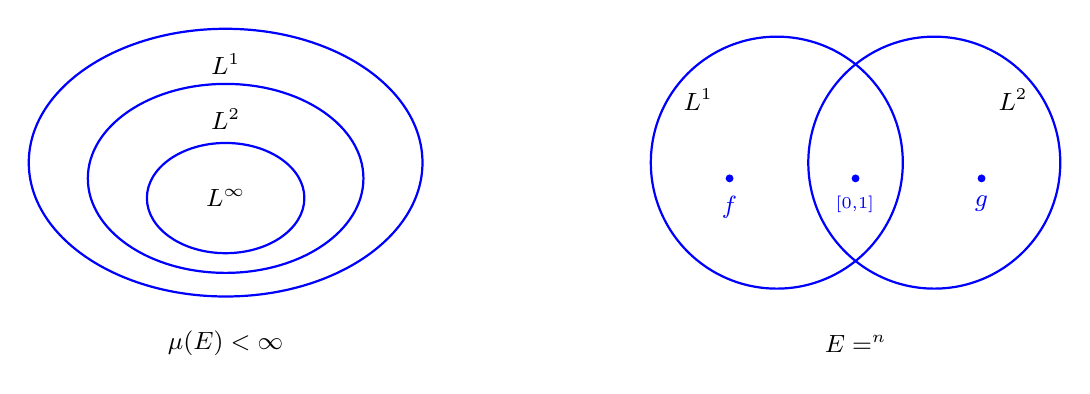
\begin{tikzpicture}[scale=1.0]
	% Left: nested, finite measure
	\begin{scope}[xshift=0cm]
		\draw[thick, color=blue] (0,0) ellipse (2.5 and 1.7);
		\draw[thick, color=blue] (0,-0.2) ellipse (1.75 and 1.2);
		\draw[thick, color=blue] (0,-0.45) ellipse (1.0 and 0.7);
		\node at (0,-0.45) {\small $L^\infty$};
		\node at (0,0.55) {\small $L^2$};
		\node at (0,1.25) {\small $L^1$};
		\node at (0,-2.3) {\small $\mu(E) < \infty$};
	\end{scope}
	% Right: overlapping, infinite measure
	\begin{scope}[xshift=8cm]
		\draw[thick, color=blue] (-1.0,0) circle (1.6);
		\draw[thick, color=blue] (1.0,0) circle (1.6);
		\node at (-2.0,0.8) {\small $L^1$};
		\node at (2.0,0.8) {\small $L^2$};
		\fill[color=blue] (-1.6,-0.2) circle (0.05);
		\node[color=blue, below] at (-1.6,-0.3) {\small $f$};
		\fill[color=blue] (1.6,-0.2) circle (0.05);
		\node[color=blue, below] at (1.6,-0.3) {\small $g$};
		\fill[color=blue] (0,-0.2) circle (0.05);
		\node[color=blue, below] at (0,-0.3) {\small $\ii_{[0,1]}$};
		\node at (0,-2.3) {\small $E = \R^n$};
	\end{scope}
\end{tikzpicture}
\end{center}

There is one general statement that survives on any measure space, and it is a useful one: the $L^p$ norms are logarithmically convex in $1/p$.

\begin{proposition}[Interpolation]\label{prop:interp}
	Let $1 \le p < r < q \le \infty$ and write $\frac 1r = \frac{\theta}{p} + \frac{1-\theta}{q}$ for some $\theta \in (0,1)$. Then for measurable $f$,
	$$\norm{f}_{L^r} \le \norm{f}_{L^p}^{\theta} \norm{f}_{L^q}^{1-\theta}.$$
	In particular $L^p \cap L^q \subseteq L^r$.
\end{proposition}

\begin{proof}
	Suppose that $q < \infty$; the case $q = \infty$ is a similar but easier variant. We factorise $|f|^r = |f|^{\theta r} |f|^{(1-\theta)r}$ and apply H\"older with the pair $p/(\theta r)$ and $q/((1-\theta)r)$, which are indeed conjugate by the definition of $\theta$:
	$$\int |f|^r \le \left( \int |f|^p \right)^{\theta r / p} \left( \int |f|^q \right)^{(1-\theta) r/q}.$$
	Taking $r$-th roots gives the result.
\end{proof}

\subsection{Density of simple functions}

Every approximation theorem in this course begins with simple functions, so let us record the basic statement.

\begin{proposition}\label{prop:simpledense}
	Let $1 \le p < \infty$. The set of simple functions $s$ with $\mu(\{s \ne 0\}) < \infty$ is dense in $L^p(E,\mu)$. For $p = \infty$, the simple functions are dense, but the finite-support condition cannot be imposed.
\end{proposition}

\begin{proof}
	Let $f \in L^p$ and, splitting into real and imaginary and then positive and negative parts, assume $f \ge 0$. Choose simple $0 \le s_n \uparrow f$ pointwise (the standard dyadic approximation does this). Then $|f - s_n|^p \le f^p \in L^1$ and $|f-s_n|^p \to 0$ pointwise, so $\norm{f - s_n}_{L^p} \to 0$ by dominated convergence. Each $s_n$ has $\mu(\{s_n \ne 0\}) < \infty$: indeed $s_n \le f$, so on $\{s_n \ge \varepsilon\}$ we have $\mu(\{s_n \ge \varepsilon\}) \le \varepsilon^{-p}\norm{f}^p_{L^p} < \infty$ by Chebyshev, and $s_n$ takes finitely many values.

	For $p = \infty$ the dyadic approximation converges uniformly on the set where $f$ is bounded, which is almost everything; but a simple function of finite support cannot approximate the constant function $1$ on $\R^n$ in $L^\infty$.
\end{proof}

Simple functions are, as their name suggests, simple, but they are not \emph{pleasant}: they are discontinuous, and one cannot differentiate them. In Section \ref{sec:mollify} we shall upgrade this density statement dramatically, to smooth compactly supported functions. That is a much more useful statement, and the mechanism which produces it -- mollification -- is one of the central tools of the course.

\subsection{Separability}

\begin{definition}
	A metric space is \vocab{separable} if it has a countable dense subset.
\end{definition}

Separability is a smallness condition, and we shall need it in two places: to run a diagonal argument in the proof of Banach--Alaoglu, and to know that $L^2$ has a countable orthonormal basis.

\begin{proposition}\label{prop:separable}
	For $1 \le p < \infty$, the space $L^p(\R^n)$ is separable. The space $L^\infty(\R^n)$ is not.
\end{proposition}

\begin{proof}
	For separability, consider the countable family $\mathcal{C}$ of finite rational linear combinations of indicators of boxes with rational vertices. Given $f \in L^p$ and $\varepsilon > 0$, Proposition \ref{prop:simpledense} produces a simple $s = \sum_{k \le N} a_k \ii_{A_k}$ with finite-measure $A_k$ and $\norm{f - s}_{L^p} < \varepsilon/2$. Each $\ii_{A_k}$ is approximated in $L^p$ by an indicator of a finite union of rational boxes, by Proposition \ref{prop:littlewood1} together with $\norm{\ii_A - \ii_B}_{L^p} = |A \triangle B|^{1/p}$; and each $a_k$ may be replaced by a nearby rational. So $\mathcal{C}$ is dense.

	For $L^\infty$, note that $\norm{\ii_{B_r(0)} - \ii_{B_s(0)}}_{L^\infty} = 1$ whenever $r \ne s$. This is an uncountable family of points pairwise at distance $1$, and no countable set can be dense in such a space (each point of the family needs its own approximant).
\end{proof}

\section{Convolution and Mollification}\label{sec:mollify}

We now come to the single most useful technique in the course. The idea is very simple. Averaging a function against a small smooth bump produces a smooth function, and if the bump is small enough the average is close to the original. So every $L^p$ function ($p< \infty$) is a limit of smooth functions, and any statement which is stable under $L^p$ limits need only be checked for smooth functions.

\subsection{Convolution}

\begin{definition}[Convolution]
	For measurable $f, g : \R^n \to \C$ we define the \vocab{convolution}
	$$(f*g)(x) = \int_{\R^n} f(y) g(x-y) \dd y,$$
	whenever the integral exists.
\end{definition}

The integral certainly exists for every $x$ when, say, $f \in L^1(\R^n)$ and $g \in L^\infty(\R^n)$, or when $f, g \in C_c(\R^n)$; we shall see in a moment exactly how much integrability is needed. The following bookkeeping lemma records the algebraic properties.

\begin{lemma}\label{lem:convalg}
	For $f, g, h \in C_c^\infty(\R^n)$ we have $f * g = g*f$ and $(f*g)*h = f*(g*h)$. Moreover
	$$\int_{\R^n} f * g = \left(\int_{\R^n} f\right)\left(\int_{\R^n} g \right).$$
\end{lemma}

\begin{proof}
	Commutativity is the substitution $z = x - y$; associativity and the last identity are Fubini together with a change of variables, all of which is justified since everything in sight is continuous and compactly supported. (The hypotheses can be weakened considerably -- for instance the last identity holds for $f, g \in L^1$ -- but this version suffices for us.)
\end{proof}

Before turning to regularity we should record when the defining integral converges, and in which space the answer lives. The following is the basic estimate, and the case $q = 1$ of it is the one we shall use on almost every subsequent page.

\begin{theorem}[Young's convolution inequality]\label{thm:youngconv}
	Let $1 \le p \le \infty$.
	\begin{enumerate}[label=(\roman*)]
		\item If $f \in L^p(\R^n)$ and $g \in L^1(\R^n)$ then $(f*g)(x)$ converges absolutely for almost every $x$, and $f * g \in L^p(\R^n)$ with
		$$\norm{f*g}_{L^p}\le\norm{f}_{L^p}\norm{g}_{L^1}.$$
		\item If $f \in L^p(\R^n)$ and $g \in L^q(\R^n)$ with $q$ conjugate to $p$, then $(f*g)(x)$ converges absolutely for \emph{every} $x$, and $f * g \in L^\infty(\R^n)$ with $\norm{f*g}_{L^\infty}\le\norm{f}_{L^p}\norm{g}_{L^q}$.
	\end{enumerate}
\end{theorem}

\begin{proof}
	(i) For $p = \infty$ this is immediate, so take $p < \infty$ and set $F(x,y) = f(x-y)g(y)$. Then for each fixed $y$,
	$$\norm{F(\cdot,y)}_{L^p}=|g(y)| \left( \int_{\R^n}|f(x-y)|^p\dd x\right)^{1/p}=|g(y)|\norm{f}_{L^p}$$
	by translation invariance of Lebesgue measure. Minkowski's integral inequality (Lemma \ref{lem:minkint}) applied to $|F|$ gives
	$$\left( \int_{\R^n}\left( \int_{\R^n}|f(x-y)g(y)|\dd y\right)^p\dd x\right)^{1/p}\le\int_{\R^n}|g(y)|\norm{f}_{L^p}\dd y = \norm{f}_{L^p}\norm{g}_{L^1}.$$
	In particular the inner integral is finite for almost every $x$, which is the absolute convergence, and the resulting function dominates $|f*g|$.

	(ii) This is H\"older applied at each fixed $x$, using that $y \mapsto f(x-y)$ has the same $L^p$ norm as $f$.
\end{proof}

\begin{remark}
	The two cases are the endpoints of the general statement: if $1 \le p,q,r\le\infty$ satisfy $\frac1p+\frac1q=1+\frac1r$ then $\norm{f*g}_{L^r}\le\norm{f}_{L^p}\norm{g}_{L^q}$. One can deduce this from the two cases above by interpolation, or prove it directly by splitting $|f(x-y)g(y)|$ into three factors and applying H\"older with three exponents. We shall not need it.
\end{remark}

Convolution is very much a smoothing operation, in a sense the next result makes precise: $f * g$ inherits the \emph{best} regularity of its two factors, not the worst. To state it we need the standard notation for higher derivatives.

\begin{definition}[Multi-index]
	An ($n$-)\vocab{multi-index} is an element $\alpha = (\alpha_1, \dots, \alpha_n) \in \Z_{\ge 0}^n$. We write $|\alpha| = \alpha_1 + \cdots + \alpha_n$ and $\alpha! = \alpha_1! \cdots \alpha_n!$, and for $x \in \R^n$ we write $x^\alpha = x_1^{\alpha_1} \cdots x_n^{\alpha_n}$. For $f \in C^k(\R^n)$ with $k \ge |\alpha|$ we write
	$$D^\alpha f = \frac{\partial^{|\alpha|} f}{\partial x_1^{\alpha_1} \cdots \partial x_n^{\alpha_n}}.$$
\end{definition}

\begin{definition}
	We say $f \in L^p_{\mathrm{loc}}(\R^n)$ if $f \ii_K \in L^p(\R^n)$ for every compact $K \subseteq \R^n$.
\end{definition}

\begin{theorem}\label{thm:convsmooth}
	Suppose $f \in L^1_{\mathrm{loc}}(\R^n)$ and $g \in C^k_c(\R^n)$ for some $k \ge 0$. Then $f * g \in C^k(\R^n)$, and $D^\alpha(f*g) = f * D^\alpha g$ for every multi-index $\alpha$ with $|\alpha| \le k$.
\end{theorem}

\begin{proof}
	Write $\tau_\xi f(x) = f(x - \xi)$ for translation. Note that $\tau_\xi(f*g) = f * (\tau_\xi g)$ straight from the definition.

	Take $k = 0$ first. Choose $R$ so large that $\supp g \subseteq B_{R-1}(0)$. As $|\xi| \to 0$ we have $\tau_\xi g \to g$ pointwise, and $|\tau_\xi g| \le (\sup |g|) \ii_{B_R(0)}$ for $|\xi| < 1$; since $f$ is locally integrable, $|f| (\sup|g|)\ii_{B_R(0)}$ is an integrable dominating function on the region that matters. Dominated convergence therefore gives $\tau_\xi (f * g) \to f*g$ pointwise, i.e.\ $f * g$ is continuous.

	Take $k = 1$. Let $\Delta^h_i g(x) = h^{-1}(g(x + he_i) - g(x))$, so $\Delta^h_i g \to D_i g$ pointwise as $h \to 0$. By the mean value theorem $\Delta^h_i g(x) = D_i g(x + te_i)$ for some $|t| \le |h|$, so $|\Delta^h_i g| \le (\sup |D_i g|)\ii_{B_R(0)}$ for $|h| < 1$, again a legitimate dominating function. Hence, by dominated convergence,
	$$\frac{(f*g)(x + he_i) - (f*g)(x)}{h} = (f * \Delta^h_i g)(x) \longrightarrow (f * D_i g)(x).$$
	So $f * g$ has partial derivatives $f * D_i g$, and these are continuous by the case $k=0$; hence $f*g \in C^1$. Induction on $k$ finishes the proof.
\end{proof}

The picture to have in mind is that of a fixed bump $g$ being slid across $f$: the value $(f * g)(x)$ is a weighted average of $f$ over a window centred at $x$, and moving the window moves the average smoothly, no matter how badly behaved $f$ is inside it.

\begin{center}
\begin{tikzpicture}[scale=1.0]
	\draw[<->] (-0.4,0) -- (7.2,0);
	\draw[<->] (0,-0.3) -- (0,2.4);
	% f: a rough, blocky function
	\draw[thick, color=gray] (0.3,0) -- (0.3,0.9) -- (1.2,0.9) -- (1.2,0.4)
		-- (2.1,0.4) -- (2.1,1.5) -- (3.0,1.5) -- (3.0,0.7) -- (4.1,0.7)
		-- (4.1,1.2) -- (5.2,1.2) -- (5.2,0.3) -- (6.3,0.3) -- (6.3,0);
	\node[color=gray] at (5.9,1.9) {\small $f$};
	% g: bump centred at 3.55 -- the averaging window
	\begin{scope}[xshift=3.55cm, xscale=0.8, yscale=0.6]
		\draw[thick, color=blue] \bumppath;
	\end{scope}
	\draw[dashed, color=blue] (3.55,0) -- (3.55,-0.25);
	\node[color=blue] at (3.55,-0.55) {\small $x$};
	\node[color=blue] at (3.55,1.35) {\small $\tau_x \check g$};
\end{tikzpicture}
\end{center}

\subsection{Approximate identities}

\begin{definition}[Mollifier]
	Fix $\phi \in C_c^\infty(\R^n)$ with $\phi \ge 0$ and $\int_{\R^n} \phi = 1$, supported in the unit ball. For $\varepsilon > 0$ set
	$$\phi_\varepsilon(y) = \varepsilon^{-n} \phi(y/\varepsilon).$$
	The family $(\phi_\varepsilon)_{\varepsilon>0}$ is called a \vocab{mollifier}, or an \vocab{approximate identity}.
\end{definition}

Each $\phi_\varepsilon$ is smooth, non-negative, supported in $B_\varepsilon(0)$, and has integral $1$ (the factor $\varepsilon^{-n}$ is exactly what is needed for this). So as $\varepsilon \downarrow 0$ the graphs become taller and narrower, converging in a sense we will make precise later to the Dirac delta.

Of course we should check such a $\phi$ exists, and the standard construction is worth seeing because the same function will reappear when we build test functions in Section \ref{sec:dist}.

\begin{example}[The standard bump]\label{aof-ex:bump}
	Define $\psi : \R \to \R$ by
	$$\psi(x) = \begin{cases} \exp\left( \dfrac{-1}{1 - x^2}\right) & |x| < 1, \\ 0 & |x| \ge 1.\end{cases}$$
	This is smooth. Away from $x = \pm 1$ this is clear. At $x = \pm 1$, every derivative of $\psi$ on $(-1,1)$ is of the form $R(x)(1-x^2)^{-m} e^{-1/(1-x^2)}$ for a polynomial $R$ and integer $m$, and $t^{-m}e^{-1/t} \to 0$ as $t \downarrow 0$ since the exponential beats every power. So every derivative extends continuously by $0$, and $\psi \in C_c^\infty(\R)$ with $\supp \psi = [-1,1]$.
\begin{center}
\begin{tikzpicture}[scale=1.0]
	\draw[ultra thin, color=lightgray, step=0.5] (-3.2,-0.2) grid (3.2,1.7);
	\draw[<->] (-3.4,0) -- (3.4,0);
	\draw[<->] (0,-0.35) -- (0,1.9);
	\draw[thick, color=blue] (-3.3,0) -- (-2.5,0);
	\begin{scope}[xscale=2.5, yscale=1.5]
		\draw[thick, color=blue] \bumppath;
	\end{scope}
	\draw[thick, color=blue] (2.5,0) -- (3.3,0);
	\node[below] at (2.5,-0.08) {\small $1$};
	\node[below] at (-2.5,-0.08) {\small $-1$};
	\draw[dashed] (0,1.5) -- (2.6,1.5);
	\node[right] at (2.65,1.5) {\small $e^{-1}$};
	\node[color=blue] at (1.55,0.45) {\small $\psi$};
\end{tikzpicture}
\end{center}
	Normalising, $\phi = \psi / \int_\R \psi$ is a legitimate mollifier on $\R$; in $\R^n$ one takes $\psi(|x|^2)$ suitably scaled, or simply a product of one-dimensional bumps. The rescaled family $\phi_\varepsilon$ concentrates as $\varepsilon \downarrow 0$:
\begin{center}
\begin{tikzpicture}[scale=1.0]
	\draw[ultra thin, color=lightgray, step=0.5] (-2.7,-0.2) grid (2.7,3.2);
	\draw[<->] (-2.9,0) -- (2.9,0);
	\draw[<->] (0,-0.35) -- (0,3.5);
	% eps = 1 : half-width 2cm, height 0.83
	\draw[thick, color=blue] (-2.8,0) -- (-2,0);
	\begin{scope}[xscale=2, yscale=0.83]
		\draw[thick, color=blue] \bumppath;
	\end{scope}
	\draw[thick, color=blue] (2,0) -- (2.8,0);
	% eps = 1/2
	\begin{scope}[xscale=1, yscale=1.66]
		\draw[thick, color=blue] \bumppath;
	\end{scope}
	% eps = 1/4
	\begin{scope}[xscale=0.5, yscale=3.31]
		\draw[thick, color=blue] \bumppath;
	\end{scope}
	\node[color=blue, right] at (1.45,0.5) {\small $\phi_{1}$};
	\node[color=blue, right] at (0.85,1.35) {\small $\phi_{1/2}$};
	\node[color=blue, right] at (0.45,2.85) {\small $\phi_{1/4}$};
\end{tikzpicture}
\end{center}
	Each of these has the same area, namely $1$.
\end{example}

Before proving that mollification converges, we need one lemma, which says that translation acts continuously on $L^p$. It is intuitively obvious and genuinely needs proof.

\begin{lemma}[Continuity of translation]\label{lem:transcont}
	Let $1 \le p < \infty$ and $g \in L^p(\R^n)$. Then $\norm{\tau_z g - g}_{L^p} \to 0$ as $z \to 0$.
\end{lemma}

\begin{proof}
	This is a density argument of exactly the shape we shall use again and again. First suppose $g = \ii_R$ for a box $R$. Then $\norm{\tau_z \ii_R - \ii_R}_{L^p}^p = |R \triangle (R + z)| \to 0$ as $z \to 0$, by direct computation with the side lengths. By linearity the result follows for finite disjoint unions of boxes.

	Next let $B$ be measurable with $|B| < \infty$. Given $\varepsilon > 0$, Proposition \ref{prop:littlewood1} gives a finite union of boxes $A$ with $\norm{\ii_A - \ii_B}_{L^p} = |A \triangle B|^{1/p}< \varepsilon$. Since translation is an isometry of $L^p$,
	$$\norm{\tau_z \ii_B - \ii_B}_{L^p} \le \norm{\tau_z \ii_B - \tau_z \ii_A}_{L^p} + \norm{\tau_z \ii_A - \ii_A}_{L^p} + \norm{\ii_A - \ii_B}_{L^p} < 3\varepsilon$$
	for $|z|$ small enough. Hence the result holds for indicators of finite-measure sets, so for simple functions of finite support, so -- again by the isometry of translation and a three-term estimate -- for all of $L^p$ by Proposition \ref{prop:simpledense}.
\end{proof}

\begin{remark}
	This fails for $p = \infty$: take $g = \ii_{[0,\infty)}$, for which $\norm{\tau_z g - g}_{L^\infty} = 1$ for every $z \ne 0$. The failure is the same one that will prevent us from approximating $L^\infty$ functions by continuous ones.
\end{remark}

\begin{theorem}[Mollification]\label{thm:mollify}
	Let $(\phi_\varepsilon)$ be a mollifier and let $g \in L^p(\R^n)$ with $1 \le p < \infty$. Then $\phi_\varepsilon * g \in C^\infty(\R^n)$, $\norm{\phi_\varepsilon * g}_{L^p} \le \norm{g}_{L^p}$, and
	$$\phi_\varepsilon * g \to g \quad \text{in } L^p(\R^n) \text{ as } \varepsilon \to 0.$$
\end{theorem}

\begin{proof}
	Smoothness is Theorem \ref{thm:convsmooth}: the convolution is defined at every point because $\int_{B_\varepsilon(x)} |g| \le \norm{g}_{L^p}\norm{\ii_{B_\varepsilon(x)}}_{L^q} < \infty$ by H\"older, so $g \in L^1_{\mathrm{loc}}$, and $\phi_\varepsilon \in C_c^\infty$.

	For the convergence, we estimate pointwise. Substituting $y = \varepsilon z$ and using $\int \phi = 1$,
	\begin{align*}
		|(\phi_\varepsilon * g)(x) - g(x)| &= \left| \int_{\R^n} \phi_\varepsilon(y) g(x - y) \dd y - g(x) \right| \\
		&= \left| \int_{\R^n} \phi(z) \big( g(x - \varepsilon z) - g(x)\big) \dd z \right| \\
		&\le \int_{\R^n} \phi(z) \left| \tau_{\varepsilon z} g(x) - g(x) \right| \dd z.
	\end{align*}
	Now take $L^p$ norms in $x$ and apply Minkowski's integral inequality (Lemma \ref{lem:minkint}) to move the norm inside the $z$-integral:
	$$\norm{\phi_\varepsilon * g - g}_{L^p} \le \int_{\R^n} \phi(z) \norm{\tau_{\varepsilon z} g - g}_{L^p} \dd z.$$
	The integrand is bounded by $2\phi(z)\norm{g}_{L^p} \in L^1$ and tends to $0$ pointwise in $z$ as $\varepsilon \to 0$, by Lemma \ref{lem:transcont}. So the integral tends to $0$ by dominated convergence. The norm bound $\norm{\phi_\varepsilon * g}_{L^p} \le \norm{g}_{L^p}$ follows from the same application of Minkowski's integral inequality without the subtraction.
\end{proof}

Here is the picture. Convolving a rough function with $\phi_\varepsilon$ rounds off its corners and jumps on the scale $\varepsilon$, and leaves it alone where it was already smooth on that scale.

\begin{center}
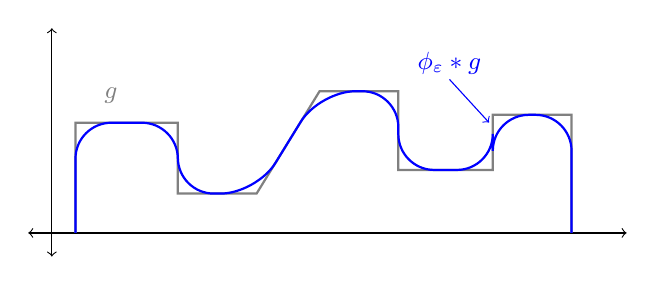
\begin{tikzpicture}[scale=1.0]
	\draw[<->] (-0.3,0) -- (7.3,0);
	\draw[<->] (0,-0.3) -- (0,2.6);
	% rough function (grey, solid, drawn first so its corners stick out)
	\draw[thick, color=gray] (0.3,0) -- (0.3,1.4) -- (1.6,1.4) -- (1.6,0.5)
		-- (2.6,0.5) -- (3.4,1.8) -- (4.4,1.8) -- (4.4,0.8) -- (5.6,0.8)
		-- (5.6,1.5) -- (6.6,1.5) -- (6.6,0);
	\node[color=gray] at (0.75,1.75) {\small $g$};
	% mollified (blue, rounded)
	\draw[thick, color=blue, rounded corners=13pt] (0.3,0) -- (0.3,1.4) -- (1.6,1.4) -- (1.6,0.5)
		-- (2.6,0.5) -- (3.4,1.8) -- (4.4,1.8) -- (4.4,0.8) -- (5.6,0.8)
		-- (5.6,1.5) -- (6.6,1.5) -- (6.6,0);
	\node[color=blue] at (5.05,2.15) {\small $\phi_\varepsilon * g$};
	\draw[color=blue, ->, shorten >=2pt] (5.05,1.95) -- (5.6,1.35);
\end{tikzpicture}
\end{center}

\begin{corollary}\label{cor:ccinftydense}
	For $1 \le p < \infty$, the space $C_c^\infty(\R^n)$ is dense in $L^p(\R^n)$.
\end{corollary}

\begin{proof}
	Given $g \in L^p$ and $\varepsilon > 0$, first truncate: $g \ii_{B_R(0)} \to g$ in $L^p$ as $R \to \infty$ by dominated convergence, so we may assume $g$ has compact support. Now $\phi_\delta * g \to g$ in $L^p$ by Theorem \ref{thm:mollify}, and $\phi_\delta * g$ is smooth with support contained in the $\delta$-neighbourhood of $\supp g$, hence compact.
\end{proof}

This is not true for $p = \infty$, and the reason is worth stating: a uniform limit of continuous functions is continuous, so no sequence in $C(\R^n)$ can converge in $L^\infty$ to a function with a genuine jump. The space $L^\infty$ is simply too big -- it is not separable either -- and this is the first of several places where it will have to be treated separately.

\begin{corollary}\label{cor:duboisreymond}
	Suppose $f \in L^1_{\mathrm{loc}}(\Omega)$ for $\Omega \subseteq \R^n$ open and
	$$\int_\Omega f \varphi \dd x = 0 \quad \text{for all } \varphi \in C_c^\infty(\Omega).$$
	Then $f = 0$ almost everywhere.
\end{corollary}

\begin{proof}
	Fix a ball $B$ with $\ol{B} \subseteq \Omega$; it suffices to show $f = 0$ a.e.\ on $B$. For $x \in B$ and $\varepsilon$ smaller than the distance from $B$ to $\partial \Omega$, the function $y \mapsto \phi_\varepsilon(x - y)$ lies in $C_c^\infty(\Omega)$, so the hypothesis gives $(\phi_\varepsilon * f)(x) = 0$. But $f \ii_B \in L^1$, so $\phi_\varepsilon * (f \ii_B) \to f\ii_B$ in $L^1$ by Theorem \ref{thm:mollify}, and for $x$ well inside $B$ these agree. Hence $f = 0$ a.e.\ on $B$.
\end{proof}

This innocuous corollary -- often called the fundamental lemma of the calculus of variations -- is what will allow us to pass from `the equation holds when tested against every smooth function' to `the equation holds'. It is used every time we solve a PDE weakly.

\subsection{The Lebesgue differentiation theorem}

Mollification says that averages of $f$ over small balls converge to $f$ in $L^p$. It is natural to ask whether they converge \emph{pointwise}, and the answer is yes, almost everywhere. This is a genuinely non-trivial theorem, and the standard proof introduces a tool -- the maximal function -- which is the beginning of a whole subject.

\begin{definition}[Hardy--Littlewood maximal function]
	For $f \in L^1(\R^n)$, define $Mf : \R^n \to [0,\infty]$ by
	$$Mf(x) = \sup_{r > 0} \frac{1}{|B_r(x)|} \int_{B_r(x)} |f(y)| \dd y.$$
\end{definition}

The maximal function is never in $L^1$ unless $f = 0$ (it decays like $|x|^{-n}$ at infinity, which is not integrable), so the best we can hope for is the following \emph{weak type} bound.

\begin{lemma}\label{aof-lem:maximal}
	Let $f \in L^1(\R^n)$. Then $Mf$ is measurable and finite almost everywhere, and there is a constant $C_n$ depending only on $n$ with
	$$\left| \{ Mf > \lambda\}\right| \le \frac{C_n \norm{f}_{L^1}}{\lambda} \quad \text{for all } \lambda > 0.$$
\end{lemma}

\begin{proof}
	Write $A_\lambda = \{Mf > \lambda\}$. For each $x \in A_\lambda$ there is $r_x > 0$ with
	$$\frac{1}{|B_{r_x}(x)|}\int_{B_{r_x}(x)} |f| > \lambda.$$
	We first check $A_\lambda$ is open (which gives measurability of $Mf$, since $A_\lambda$ is a superlevel set). If $x_m \to x$ with $x \in A_\lambda$, then $\ii_{B_{r_x}(x_m)} \to \ii_{B_{r_x}(x)}$ almost everywhere and dominated convergence gives
	$$\frac{1}{|B_{r_x}(x_m)|}\int_{B_{r_x}(x_m)} |f| \longrightarrow \frac{1}{|B_{r_x}(x)|}\int_{B_{r_x}(x)}|f| > \lambda,$$
	so $x_m \in A_\lambda$ for large $m$. Thus the complement of $A_\lambda$ is closed under limits, i.e.\ $A_\lambda$ is open.

	Now let $K \subseteq A_\lambda$ be compact. The balls $\{B_{r_x}(x) : x \in A_\lambda\}$ cover $K$, so finitely many $B_1, \dots, B_N$ do. By the Wiener covering lemma there is a disjoint subcollection $B_{i_1}, \dots, B_{i_k}$ with $\left| \bigcup_{i \le N} B_i \right| \le 3^n \sum_{j \le k} |B_{i_j}|$. Hence
	$$|K| \le 3^n \sum_{j=1}^k |B_{i_j}| \le \frac{3^n}{\lambda}\sum_{j=1}^k \int_{B_{i_j}}|f| \le \frac{3^n}{\lambda}\int_{\R^n}|f| = \frac{3^n \norm{f}_{L^1}}{\lambda},$$
	using disjointness in the last inequality. Taking the supremum over compact $K \subseteq A_\lambda$ and using inner regularity gives $|A_\lambda| \le 3^n \norm{f}_{L^1}/\lambda$. Finally $\{Mf = \infty\} \subseteq A_\lambda$ for every $\lambda$, so it is null.
\end{proof}

\begin{theorem}[Lebesgue differentiation theorem]\label{thm:lebdiff}
	Let $f \in L^1(\R^n)$. Then for almost every $x \in \R^n$,
	$$\lim_{r \to 0} \frac{1}{|B_r(x)|} \int_{B_r(x)} |f(y) - f(x)| \dd y = 0.$$
	Such $x$ are called \vocab{Lebesgue points} of $f$.
\end{theorem}

The idea of the proof is a beautiful one and is used throughout analysis: the statement is trivially true for continuous functions, continuous functions are dense, and the maximal inequality controls the error made in passing to the limit. This last ingredient is essential -- density alone is never enough for a pointwise statement.

\begin{proof}
	For $\lambda > 0$ let
	$$A_\lambda = \left\{ x \in \R^n : \limsup_{r \to 0}\frac{1}{|B_r(x)|}\int_{B_r(x)}|f(y)-f(x)| \dd y > 2\lambda \right\};$$
	it is enough to show $|A_\lambda| = 0$ for every $\lambda > 0$.

	Fix $\varepsilon > 0$ and, by Corollary \ref{cor:ccinftydense}, choose $g \in C_c^\infty(\R^n)$ with $\norm{f - g}_{L^1} < \varepsilon$. For any $x$ and $r$, the triangle inequality gives
	\begin{align*}
		\frac{1}{|B_r(x)|}\int_{B_r(x)}|f(y) - f(x)| \dd y &\le \frac{1}{|B_r(x)|}\int_{B_r(x)}|f(y) - g(y)|\dd y \\
		&\quad + \frac{1}{|B_r(x)|}\int_{B_r(x)}|g(y) - g(x)| \dd y + |g(x) - f(x)|.
	\end{align*}
	The first term is at most $M_{f-g}(x)$ by definition, and the second tends to $0$ as $r \to 0$ by continuity of $g$. So
	$$\limsup_{r \to 0}\frac{1}{|B_r(x)|}\int_{B_r(x)}|f(y)-f(x)|\dd y \le M_{f-g}(x) + |f(x) - g(x)|.$$
	Consequently, if $x \in A_\lambda$ then either $M_{f-g}(x) > \lambda$ or $|f(x)-g(x)| > \lambda$. By Lemma \ref{aof-lem:maximal} the first set has measure at most $C_n \varepsilon/\lambda$, and by Chebyshev's inequality the second has measure at most $\varepsilon/\lambda$. Hence
	$$|A_\lambda| \le \frac{(1 + C_n)\varepsilon}{\lambda},$$
	and since $\varepsilon > 0$ was arbitrary, $|A_\lambda| = 0$.
\end{proof}

\begin{corollary}
	For $f \in L^1(\R^n)$ and any mollifier $(\phi_\varepsilon)$, we have $\phi_\varepsilon * f \to f$ almost everywhere as $\varepsilon \to 0$.
\end{corollary}

\begin{proof}
	At a Lebesgue point $x$, bounding $\phi_\varepsilon \le \norm{\phi}_{L^\infty}\varepsilon^{-n}\ii_{B_\varepsilon(0)}$ gives
	$$|(\phi_\varepsilon * f)(x) - f(x)| \le \int \phi_\varepsilon(y)|f(x-y)-f(x)| \dd y \le \frac{C}{|B_\varepsilon(x)|}\int_{B_\varepsilon(x)}|f(y)-f(x)|\dd y,$$
	which tends to $0$.
\end{proof}

\begin{corollary}\label{cor:ftc}
	Let $g \in L^1(\R)$ and set $G(x) = \int_{-\infty}^x g(t) \dd t$. Then $G$ is differentiable at almost every $x$, with $G'(x) = g(x)$.
\end{corollary}

\begin{proof}
	At a Lebesgue point $x$ of $g$ we have, for $h > 0$,
	\begin{align*}
		\left| \frac{G(x+h)-G(x)}{h} - g(x) \right| &= \left|\frac 1h \int_x^{x+h} (g(t)-g(x))\dd t \right| \\
		&\le \frac{2}{|B_h(x)|}\int_{B_h(x)}|g-g(x)| \to 0,
	\end{align*}
	and similarly for $h < 0$.
\end{proof}

\begin{example}
	Take $g = \ii_{(0,\infty)}$ on $\R$ (which is in $L^1_{\mathrm{loc}}$, and the theorem applies locally). Every $x \ne 0$ is a Lebesgue point, and indeed
	$$G(x) = \int_{-\infty}^x g = \begin{cases} 0 & x \le 0 \\ x & x > 0\end{cases}$$
	is differentiable exactly off $0$, with $G' = g$ there. The point $x=0$ is not a Lebesgue point, and this single bad point is the seed from which the whole theory of distributions grows: we would very much like to say that $G' = g$ and $g' = \delta_0$, and presently we shall.
\end{example}

\section{Hilbert Space and Duality}\label{sec:duality}

We turn now to the linear structure. The spaces $L^p$ are Banach spaces, and $L^2$ is a Hilbert space; the point of this section is to see what that buys us. The headline results are a complete description of the dual space of $L^p$ for $p < \infty$, and -- as a by-product of the Hilbert space geometry -- a proof of the Radon--Nikod\'ym theorem, which is a theorem of measure theory obtained by functional-analytic means. That last is characteristic of the subject: once the spaces are set up correctly, hard-looking measure theory becomes soft linear algebra.

\subsection{Orthogonal systems of functions}

Throughout, $\Hil$ denotes a Hilbert space over $\C$ with inner product $\ip{\cdot}{\cdot}$, conjugate-linear in the first variable. The model to keep in mind is $\Hil = L^2(E,\mu)$ with $\ip{f}{g} = \int_E \bar f g \dd \mu$.

\begin{definition}
	A subset $S = \{u_j\}_{j \in J} \subseteq \Hil$ is \vocab{orthogonal} if $\ip{u_i}{u_j} = 0$ whenever $i \ne j$, and \vocab{orthonormal} if in addition $\norm{u_j} = 1$ for all $j$. We say $S$ is \vocab{complete} if $\ol{\spn S} = \Hil$, and an orthonormal complete set is an \vocab{orthonormal basis}. A Hilbert space is \vocab{separable} exactly when it admits a countable orthonormal basis.
\end{definition}

If $\{e_n\}_{n \in \N}$ is a countable orthonormal basis then every $x \in \Hil$ has the expansion
$$x = \sum_{n \in \N} \ip{e_n}{x} e_n, \qquad \norm{x}^2 = \sum_{n \in \N} |\ip{e_n}{x}|^2,$$
the series converging in norm; this is Parseval's identity, and it says that $\Hil \cong \ell^2$ as soon as $\Hil$ is separable and infinite-dimensional. Abstractly, then, there is only one separable infinite-dimensional Hilbert space. What makes the subject non-trivial is that the \emph{same} space carries many different natural bases, and that choosing a good one is often the whole problem.

\begin{example}\label{ex:onb}
	Some orthonormal bases worth knowing.
	\begin{enumerate}[label=(\roman*)]
		\item The trigonometric system $\{x \mapsto e^{-2\pi i n x} : n \in \Z\}$ is an orthonormal basis of $L^2((0,1))$. Orthonormality is a computation; completeness follows either from Stone--Weierstrass (the trigonometric polynomials are dense in the continuous periodic functions in the uniform norm) or from Corollary \ref{cor:ccinftydense}. This is the classical theory of Fourier series, in one line.
		\item Let
		$$\psi(x) = \begin{cases} 1 & 0 \le x < 1/2, \\ -1 & 1/2 \le x < 1, \\ 0 & \text{otherwise},\end{cases}$$
		and set $\psi_{n,k}(x) = 2^{n/2}\psi(2^n x - k)$. Then $\{\psi_{n,k} : n, k \in \Z\}$ is an orthonormal basis of $L^2(\R)$, the \vocab{Haar system}. It is the simplest example of a wavelet basis, and unlike the trigonometric system its elements are localised in space as well as in frequency.
		\item Let $\Hil = L^2(\R, e^{-x^2}\dd x)$, with inner product $\ip{f}{g} = \int_\R \ol{f} g e^{-x^2} \dd x$. Applying Gram--Schmidt to the linearly independent family $1, x, x^2, \dots$ produces orthogonal polynomials $H_k$ with $\deg H_k = k$; normalised so that the coefficient of $x^k$ in $H_k$ is $2^k$, these are the \vocab{Hermite polynomials}, and they form a complete orthogonal set.
	\end{enumerate}
\end{example}

The result from Linear Analysis we shall use over and over is the following.

\begin{theorem}[Riesz representation, Hilbert space form]\label{thm:rieszhilbert}
	Let $\Hil$ be a Hilbert space and $\Lambda : \Hil \to \C$ a bounded linear functional. Then there is a unique $w \in \Hil$ with
	$$\Lambda u = \ip{w}{u} \quad \text{for all } u \in \Hil,$$
	and $\norm{\Lambda}_{\Hil'} = \norm{w}$.
\end{theorem}

\begin{proof}
	We recall the argument. If $\Lambda = 0$ take $w = 0$. Otherwise $K = \ker \Lambda$ is a proper closed subspace, so there is $v \in K^\perp$ with $\norm{v} = 1$ (take any $z \notin K$ and subtract its orthogonal projection onto $K$, which exists because $K$ is closed and convex). For any $u$, the vector $u - \frac{\Lambda u}{\Lambda v} v$ lies in $K$, hence is orthogonal to $v$, so $\ip{v}{u} = \frac{\Lambda u}{\Lambda v}$. Thus $w = \ol{\Lambda v} v$ works. Uniqueness and the norm identity are immediate.
\end{proof}

\subsection{The Radon--Nikod\'ym theorem}

Here is a first illustration of the power of Theorem \ref{thm:rieszhilbert}.

\begin{definition}
	Let $\mu, \nu$ be measures on a measurable space $(E, \mathcal{E})$. We say $\nu$ is \vocab{absolutely continuous} with respect to $\mu$, written $\nu \ll \mu$, if $\mu(A) = 0 \implies \nu(A) = 0$ for all $A \in \mathcal{E}$. We say $\mu$ and $\nu$ are \vocab{mutually singular}, written $\mu \perp \nu$, if there is a measurable $Z$ with $\mu(Z) = 0 = \nu(Z^c)$.
\end{definition}

\begin{theorem}[Radon--Nikod\'ym]\label{thm:radonnikodym}
	Let $\mu, \nu$ be finite measures on $(E,\mathcal{E})$ with $\nu \ll \mu$. Then there is a non-negative $w \in L^1(E,\mu)$ such that
	$$\nu(A) = \int_A w \dd \mu \quad \text{for all } A \in \mathcal{E};$$
	equivalently, $\int_E F \dd \nu = \int_E F w \dd\mu$ for every measurable $F : E \to [0,\infty]$.
\end{theorem}

\begin{proof}
	The trick is to introduce two auxiliary measures which are comparable to both $\mu$ and $\nu$. Set $\alpha = \mu + 2\nu$ and $\beta = \nu + 2\mu$, both finite. Since $\mu \le \alpha$ and $\nu \le \alpha$, we have
	$$\Hil := L^2(E,\alpha) \subseteq L^2(E,\mu) \cap L^2(E,\nu),$$
	and every $f \in \Hil$ is $\beta$-integrable. Consider the linear functional
	$$\Lambda(f) = \int_E f \dd \beta, \qquad f \in \Hil.$$
	It is bounded, since
	$$|\Lambda(f)| \le \int_E |f| \dd \beta = 2\int_E |f| \dd\mu + \int_E |f| \dd\nu \le 2\int_E |f| \dd \alpha \le 2\sqrt{\alpha(E)}\norm{f}_{L^2(\alpha)}$$
	by Cauchy--Schwarz. By Theorem \ref{thm:rieszhilbert} there is $g \in \Hil$ with
	$$\int_E f \dd \beta = \int_E gf \dd \alpha \quad \text{for all } f \in \Hil.$$
	Unwinding the definitions of $\alpha$ and $\beta$, this says
	\begin{equation*}
		\int_E (2g-1) f \dd \nu = \int_E (2 - g) f \dd \mu \quad \text{for all } f \in \Hil. \tag{$\ast$}
	\end{equation*}

	We claim $\tfrac 12 \le g \le 2$ almost everywhere with respect to both $\mu$ and $\nu$. Indeed, let $A_j = \{g < \tfrac 12 - \tfrac 1j\}$ and put $f = \ii_{A_j}$ in $(\ast)$:
	$$\frac{3}{2}\mu(A_j) \le \int_E (2-g)\ii_{A_j} \dd \mu = \int_E (2g-1)\ii_{A_j}\dd\nu \le -\frac{2}{j}\nu(A_j) \le 0,$$
	forcing $\mu(A_j) = 0$ and then $\nu(A_j) = 0$. Letting $j \to \infty$ gives $g \ge 1/2$ a.e.; the argument at the other end, with $A_j = \{g > 2 + 1/j\}$, gives $g \le 2$ a.e.

	Now let $Z = \{g = 1/2\}$. Putting $f = \ii_Z$ in $(\ast)$ gives $0 = \int_Z (2-g) \dd\mu \ge \tfrac 32 \mu(Z)$, so $\mu(Z) = 0$, and hence $\nu(Z) = 0$ by absolute continuity. Given measurable $F : E \to [0,\infty]$, define on $Z^c$
	$$f = \frac{F}{2g-1}, \qquad w = \frac{2-g}{2g-1},$$
	and $f = w = 0$ on $Z$. Both are well defined and bounded multiples of $F$ and $1$ respectively, since $2g - 1 \in [0,3]$ is bounded away from $0$ off $Z$ after a further exhaustion, and applying $(\ast)$ (first for bounded $F$, then in general by monotone convergence) gives
	$$\int_E F \dd \nu = \int_{Z^c} (2g-1)f \dd\nu = \int_{Z^c}(2-g) f \dd\mu = \int_E Fw \dd\mu$$
	as required. Taking $F = 1$ shows $w \in L^1(E,\mu)$, and taking $F = \ii_A$ gives the stated form.
\end{proof}

\subsection{Dual spaces}

\begin{definition}[Dual space]
	Let $X$ be a topological vector space over $\F = \R$ or $\C$. The \vocab{(topological) dual} $X'$ is the vector space of continuous linear functionals $\Lambda : X \to \F$. If $X$ is normed, we norm $X'$ by
	$$\norm{\Lambda}_{X'} = \sup_{\norm{x}_X \le 1} |\Lambda(x)|.$$
\end{definition}

The space $X'$ is always a Banach space, complete regardless of whether $X$ is, since completeness is inherited from the target field. What is not at all obvious is that $X'$ contains anything: the definition alone does not produce a single non-zero functional. That is the business of the Hahn--Banach theorem, which we prove in Section \ref{sec:weak}; for now we record what we shall need.

\begin{lemma}\label{lem:seppoints}
	Let $X$ be a normed space and $x \ne y$ in $X$. Then there is $\Lambda \in X'$ with $\Lambda(x) \ne \Lambda(y)$.
\end{lemma}

We defer the proof to Corollary \ref{cor:hbsep}. Granting it, for each $x \in X$ the evaluation map $f_x : X' \to \F$, $\Lambda \mapsto \Lambda(x)$, is linear and bounded (with $|f_x(\Lambda)| \le \norm{x}\norm{\Lambda}$), hence $f_x \in X'' = (X')'$; and Lemma \ref{lem:seppoints} says $x \mapsto f_x$ is injective. In fact it is isometric, again by Hahn--Banach.

\begin{definition}[Reflexive]
	A Banach space $X$ is \vocab{reflexive} if the canonical map $X \to X''$, $x \mapsto f_x$, is surjective (hence an isometric isomorphism), in which case we write $X = X''$.
\end{definition}

For a Hilbert space, Theorem \ref{thm:rieszhilbert} gives a conjugate-linear isometry $\Hil \to \Hil'$; applying it twice shows that every Hilbert space is reflexive. This will matter enormously later: reflexivity is what makes bounded sequences have weakly convergent subsequences.

\subsection{The dual of \texorpdfstring{$L^p$}{Lp}}

Fix a measure space $(E,\mathcal{E},\mu)$ and conjugate exponents $p,q$. H\"older's inequality says that for $g \in L^q$ the map
$$\Lambda_g(f) = \int_E gf \dd \mu$$
is a bounded linear functional on $L^p$ with $\norm{\Lambda_g}_{(L^p)'} \le \norm{g}_{L^q}$. In fact equality holds.

\begin{lemma}\label{lem:isometricdual}
	For $1 \le p \le \infty$ and $g \in L^q$ we have $\norm{\Lambda_g}_{(L^p)'} = \norm{g}_{L^q}$. Hence $\kappa : L^q \to (L^p)'$, $g \mapsto \Lambda_g$, is a linear isometry.
\end{lemma}

\begin{proof}
	Only `$\ge$' needs proof. Suppose $1 < q < \infty$ and $g \ne 0$; take
	$$f = \frac{|g|^{q-1}\ol{\sgn g}}{\norm{g}_{L^q}^{q-1}}, \quad \text{so that} \quad \norm{f}_{L^p}^p = \frac{\int |g|^{(q-1)p}}{\norm{g}^{(q-1)p}_{L^q}} = 1$$
	since $(q-1)p = q$. Then $\Lambda_g(f) = \norm{g}_{L^q}$. For $q = 1$ take $f = \ol{\sgn g}$, of $L^\infty$ norm $1$. For $q = \infty$, given $\varepsilon > 0$ let $A = \{|g| > \norm{g}_{L^\infty} - \varepsilon\}$, which has positive measure; assuming $\mu$ $\sigma$-finite we may shrink it to have finite positive measure, and $f = \mu(A)^{-1}\ii_A \ol{\sgn g}$ has $\norm{f}_{L^1} = 1$ and $\Lambda_g(f) \ge \norm{g}_{L^\infty}-\varepsilon$.
\end{proof}

So $L^q$ sits isometrically inside $(L^p)'$. The theorem is that for $p < \infty$ it is everything.

\begin{theorem}\label{thm:lpdual}
	Let $(E, \mathcal{E},\mu)$ be $\sigma$-finite, let $1 \le p < \infty$ and let $q$ be conjugate to $p$. Then $\kappa : L^q(E,\mu) \to L^p(E,\mu)'$ is an isometric isomorphism. We write $L^p(E,\mu)' = L^q(E,\mu)$.
\end{theorem}

\begin{proof}
	By Lemma \ref{lem:isometricdual} it remains to prove surjectivity, and by Lemma \ref{lem:isometricdual} again it is enough to produce, for each $\Lambda \in (L^p)'$, some $g \in L^q$ with $\Lambda = \Lambda_g$.

	\emph{Reduction to real scalars and positive functionals.} Writing $f = f_r + i f_i$ and $\Lambda_r(f) = \re \Lambda(f)$, $\Lambda_i(f) = \im \Lambda(f)$ for real $f$, a complex functional is determined by a pair of real ones, so we may take the scalars real. A real-linear bounded $\Lambda : L^p(E;\R) \to \R$ is called \vocab{positive} if $\Lambda(f) \ge 0$ whenever $f \ge 0$; one checks (this is on the example sheet, and is the Jordan decomposition in disguise) that every bounded real-linear functional is a difference $\Lambda = \Lambda^+ - \Lambda^-$ of positive bounded ones. So assume $\Lambda$ positive.

	\emph{The finite measure case.} Suppose first $\mu(E) < \infty$. Define $\nu(A) = \Lambda(\ii_A)$ for $A \in \mathcal{E}$. Then $\nu \ge 0$ by positivity, $\nu(\emptyset) = 0$, and $\nu$ is finitely additive by linearity. It is countably additive: if $B = \bigcup_{n \ge 1} A_n$ with the $A_n$ disjoint, and $B_k = \bigcup_{n \le k}A_n$, then
	$$\norm{\ii_B - \ii_{B_k}}_{L^p} = \mu(B \setminus B_k)^{1/p} \to 0,$$
	so $\nu(B) - \nu(B_k) = \Lambda(\ii_{B} - \ii_{B_k}) \to 0$ by continuity of $\Lambda$. The same computation shows $\mu(A) = 0 \implies \nu(A) = 0$, i.e.\ $\nu \ll \mu$. By Theorem \ref{thm:radonnikodym} there is a non-negative $g \in L^1(E,\mu)$ with $\Lambda(\ii_A) = \int_A g \dd\mu$ for all $A$; by linearity $\Lambda(f) = \int_E fg \dd\mu$ for all simple $f$, and hence for all bounded measurable $f$ by dominated convergence.

	\emph{$g$ lies in $L^q$.} Suppose $1 < p < \infty$. For $N > 0$ let $g_N = \min(g, N)$ and $f_N = g_N^{q-1}$, a bounded function. Then
	$$\int_E g_N^{q} \dd\mu \le \int_E f_N g \dd\mu = \Lambda(f_N) \le \norm{\Lambda} \norm{f_N}_{L^p} = \norm{\Lambda}\left( \int_E g_N^{q}\dd\mu\right)^{1/p},$$
	using $(q-1)p = q$. Dividing (the integral is finite as $g_N$ is bounded and $\mu(E) < \infty$) gives $\norm{g_N}_{L^q} \le \norm{\Lambda}$, and monotone convergence as $N \to \infty$ gives $\norm{g}_{L^q}\le \norm{\Lambda} < \infty$. For $p = 1$ one argues instead that $\mu(\{g > \norm{\Lambda}+\varepsilon\}) = 0$, directly from $\Lambda(\ii_A) \le \norm{\Lambda}\mu(A)$, so $g \in L^\infty$. Finally, since $g \in L^q$ the functional $\Lambda_g$ is bounded on $L^p$ and agrees with $\Lambda$ on the dense set of simple functions (Proposition \ref{prop:simpledense}), so $\Lambda = \Lambda_g$.

	\emph{The $\sigma$-finite case.} Write $E = \bigcup_k E_k$ with $E_k \uparrow$ and $\mu(E_k) < \infty$. Applying the above on each $E_k$ produces $g_k \in L^q(E_k)$ representing $\Lambda$ on functions supported in $E_k$; by uniqueness these are consistent, so they patch to a measurable $g$ on $E$ with $\norm{g \ii_{E_k}}_{L^q}\le\norm{\Lambda}$ for every $k$. Monotone convergence gives $g \in L^q$ with $\norm{g}_{L^q}\le\norm{\Lambda}$, and $\Lambda = \Lambda_g$ on the dense set of functions supported in some $E_k$, hence everywhere.
\end{proof}

\begin{corollary}\label{cor:lpreflexive}
	For $1 < p < \infty$, $L^p(\R^n)$ is reflexive.
\end{corollary}

\begin{proof}
	$(L^p)'' = (L^q)' = L^p$, and one checks that the composite isomorphism is the canonical embedding.
\end{proof}

The theorem genuinely fails at $p = \infty$: the dual of $L^\infty$ is much larger than $L^1$. To see this, note that $C([0,1]) \subseteq L^\infty([0,1])$ and $f \mapsto f(0)$ is a bounded functional on $C([0,1])$; Hahn--Banach extends it to $L^\infty$, and no $g \in L^1$ can represent it (it vanishes on every $f$ vanishing near $0$, which forces $g = 0$ a.e., but the functional is not zero). Correspondingly neither $L^1$ nor $L^\infty$ is reflexive. This is not a technicality to be regretted: it is why the natural home for many variational problems is $L^p$ with $1 < p< \infty$, and why problems formulated in $L^1$ (or in the space of measures) are genuinely harder.

\subsection{The Riesz representation theorem for measures}

There is one more duality worth recording, and it goes the other way: instead of describing functionals in terms of functions, it describes them in terms of \emph{measures}. This is the sense in which a measure `is' a way of integrating continuous functions.

\begin{definition}
	Let $E$ be a topological space and $\mathcal{E} \supseteq \mathcal{B}(E)$ a $\sigma$-algebra. A measure $\mu$ on $(E,\mathcal{E})$ is \vocab{regular} if for every $A \in \mathcal{E}$ and $\varepsilon > 0$ there are a closed $C$ and an open $O$ with $C \subseteq A \subseteq O$ and $\mu(O \setminus C) < \varepsilon$.
\end{definition}

Lebesgue measure on $(\R^n, \mathcal{M})$ is regular, by Theorem \ref{aof-thm:lebesgue}(iii). Now if $\mu$ is a finite regular measure on $\R^n$, then every $f \in C^0_c(\R^n;\R)$ is measurable and bounded, so
$$\Lambda(f) = \int_{\R^n} f \dd \mu$$
defines a positive bounded linear functional on $C^0_c(\R^n;\R)$. The question is whether $\mu$ can be recovered from $\Lambda$, and whether every such $\Lambda$ arises this way.

\begin{lemma}\label{lem:measuredetermined}
	A finite regular measure $\mu$ on $\R^n$ is determined by the functional $\Lambda(f) = \int f \dd\mu$ on $C_c^0(\R^n;\R)$.
\end{lemma}

\begin{proof}
	We would like to take $f = \ii_A$, but indicators are not continuous, so we approximate. Let $O$ be open, and for $k \in \N$ set $O_k = O \cap \{|x| < k\}$ and
	$$\chi_k(x) = \begin{cases} 1 & x \in O_k, \ \dist(x, O_k^c) \ge 1/k, \\ k\dist(x, O_k^c) & x \in O_k, \ \dist(x,O_k^c) < 1/k, \\ 0 & x \notin O_k.\end{cases}$$
	Each $\chi_k$ is continuous with compact support (distance functions are $1$-Lipschitz) and $\chi_k \uparrow \ii_O$ pointwise. By monotone convergence $\Lambda(\chi_k) \to \mu(O)$. So $\Lambda$ determines $\mu$ on open sets, and hence on all of $\mathcal{E}$ by regularity.
\end{proof}

\begin{theorem}[Riesz--Markov]\label{thm:rieszmarkov}
	Let $\Lambda : C_c^0(\R^n;\R) \to \R$ be a positive bounded linear functional. Then there is a $\sigma$-algebra $\mathcal{M} \supseteq \mathcal{B}(\R^n)$ and a unique finite regular measure $\mu$ on it with
	$$\Lambda(f) = \int_{\R^n} f \dd \mu \quad \text{for all } f \in C_c^0(\R^n;\R).$$
\end{theorem}

The proof is a construction of $\mu$ from $\Lambda$ by an outer measure argument -- one defines $\mu(O) = \sup\{\Lambda(f) : 0 \le f \le 1, \supp f \subseteq O\}$ for open $O$ and extends by regularity -- and it is genuinely technical. We shall take it on trust.

\begin{example}
	Take $\Lambda(f) = f(0)$. This is positive and bounded, and the measure it represents is $\mu = \delta_0$, the Dirac point mass at the origin. The reader who feels that $\delta_0$ `should' be a function will be pleased to know that in Section \ref{sec:dist} it becomes a perfectly respectable distribution, and that this example is the prototype.
\end{example}

\section{Weak Topologies and Compactness}\label{sec:weak}

In finite dimensions, the Bolzano--Weierstrass theorem says that bounded sequences have convergent subsequences, and this single fact underlies most existence proofs in analysis: to produce an object with a desired property, construct a bounded sequence of approximations and pass to a limit. In infinite dimensions this fails completely. In $\ell^2$ the orthonormal sequence $(e_n)$ is bounded but $\norm{e_n - e_m} = \sqrt 2$ for $n \ne m$, so no subsequence is Cauchy; indeed the closed unit ball of a normed space is compact if and only if the space is finite-dimensional.

The remedy is to keep the sequence and change the topology. If we declare fewer sets to be open, more sets become compact, and with luck we can weaken the topology enough to restore Bolzano--Weierstrass while keeping enough separation to make the limits useful. This section carries that out. We need the Hahn--Banach theorem first, because a weak topology is built from linear functionals and is useless unless there are plenty of them.

\subsection{The Hahn--Banach theorem}

Hahn--Banach is an extension theorem: a bounded functional defined on a subspace extends to the whole space with the same bound. We work over $\R$; the complex case follows by taking real parts, since a complex-linear $\Lambda$ is determined by $\ell = \re \Lambda$ via $\Lambda(x) = \ell(x) - i \ell(ix)$.

For the sake of generality we replace the norm bound by something weaker.

\begin{definition}[Sublinear functional]
	A \vocab{sublinear functional} on a real vector space $X$ is a map $p : X \to \R$ with
	$$p(x+y) \le p(x) + p(y), \qquad p(tx) = tp(x)$$
	for all $x,y \in X$ and $t \ge 0$.
\end{definition}

\begin{example}
	Every seminorm is sublinear, and so is $|\ell|$ for any linear $\ell$. But sublinear functionals need not be non-negative or symmetric: on $\R$, $p(x) = x$ is sublinear.
\end{example}

Note that a one-sided bound $\ell(x) \le p(x)$ automatically gives a two-sided one, since $-\ell(x) = \ell(-x) \le p(-x)$, whence $-p(-x) \le \ell(x) \le p(x)$.

\begin{lemma}[Banach extension lemma]\label{lem:banachext}
	Let $X$ be a real vector space, $p$ a sublinear functional on $X$, $M \le X$ a subspace, and $\ell : M \to \R$ linear with $\ell \le p$ on $M$. Then for any $x \in X \setminus M$ there is a linear $\wt\ell$ on $\wt M = \spn(M \cup \{x\})$ extending $\ell$ with $\wt\ell \le p$ on $\wt M$.
\end{lemma}

\begin{proof}
	Every $w \in \wt M$ is uniquely $w = \lambda x + y$ with $y \in M$, $\lambda \in \R$, so $\wt \ell$ is determined by the single number $a = \wt\ell(x)$, and the problem is to choose $a$ compatibly.

	For $y, z \in M$ we have
	$$\ell(y) + \ell(z) = \ell(y+z) \le p(y+z) \le p(y - x) + p(z+x),$$
	so that $\ell(y) - p(y-x) \le p(z+x) - \ell(z)$ for all $y,z \in M$. Hence
	$$a := \sup_{y \in M} \big( \ell(y) - p(y-x)\big) \le \inf_{z \in M}\big( p(z+x)-\ell(z)\big) < \infty,$$
	and both bounds are finite. By construction $\ell(y) - a \le p(y - x)$ and $\ell(z) + a \le p(z+x)$ for all $y, z \in M$. Now take $w = \lambda x + y$. For $\lambda > 0$, apply the second inequality with $z = \lambda^{-1}y$ and multiply by $\lambda$; for $\lambda < 0$, apply the first with $y' = -\lambda^{-1}y$ and multiply by $-\lambda$; for $\lambda = 0$ there is nothing to prove. In each case we get $\wt\ell(w) \le p(w)$.
\end{proof}

If $X/M$ is finite-dimensional we can now finish by induction, and if $X$ is separable we can finish by a countable induction plus a limiting argument. In general we need a form of the axiom of choice.

\begin{proposition}[Zorn's lemma]\label{prop:zorn}
	Let $(S, \le)$ be a non-empty partially ordered set in which every totally ordered subset has an upper bound. Then $S$ has a maximal element.
\end{proposition}

\begin{theorem}[Hahn--Banach]\label{thm:hahnbanach}
	Let $X$ be a real vector space, $p$ a sublinear functional on $X$, $M \le X$ and $\ell : M \to \R$ linear with $\ell \le p$ on $M$. Then there is a linear $\wt\ell : X \to \R$ extending $\ell$ with $\wt\ell \le p$ on $X$.
\end{theorem}

\begin{proof}
	Let $S$ be the set of pairs $(N, \ell^*)$ where $M \le N \le X$ and $\ell^* : N \to \R$ is linear, extends $\ell$, and satisfies $\ell^* \le p$ on $N$. Order $S$ by $(N_1,\ell_1^*) \le (N_2,\ell_2^*)$ if $N_1 \le N_2$ and $\ell_2^*$ extends $\ell_1^*$. Then $S \ne \emptyset$ (it contains $(M,\ell)$), and any chain $T \subseteq S$ has the upper bound $(N_T, \ell_T)$ with $N_T = \bigcup_{(N,\ell^*) \in T} N$ -- a subspace because $T$ is totally ordered -- and $\ell_T$ the common value. By Proposition \ref{prop:zorn} there is a maximal $(\wt N, \wt\ell)$; and if $\wt N \ne X$ then Lemma \ref{lem:banachext} would extend it further, contradicting maximality. So $\wt N = X$.
\end{proof}

\begin{corollary}\label{cor:hbnorm}
	Let $X$ be a normed space over $\F = \R$ or $\C$, $M \le X$, and $\Lambda : M \to \F$ a bounded linear functional. Then there is $\wt \Lambda \in X'$ extending $\Lambda$ with $\norm{\wt\Lambda}_{X'} = \norm{\Lambda}_{M'}$.
\end{corollary}

\begin{proof}
	For $\F = \R$ apply Theorem \ref{thm:hahnbanach} with $p(x) = \norm{\Lambda}_{M'}\norm{x}$. For $\F = \C$, write $\Lambda(x) = \ell(x) - i\ell(ix)$ with $\ell = \re \Lambda$ real-linear; since for each $x$ we may pick $\theta$ with $|\Lambda(x)| = \ell(e^{i\theta}x)$, the real and complex norms agree, and extending $\ell$ then setting $\wt\Lambda(x) = \wt\ell(x) - i\wt\ell(ix)$ does the job.
\end{proof}

\begin{corollary}\label{cor:hbnormattained}
	For any $x \ne 0$ in a normed space $X$ there is $\Lambda \in X'$ with $\norm{\Lambda}_{X'} = 1$ and $\Lambda(x) = \norm{x}$. Consequently $\norm{x} = \sup_{\norm{\Lambda}_{X'}\le 1}|\Lambda(x)|$, and the canonical map $X \to X''$ is isometric.
\end{corollary}

\begin{proof}
	Define $\Lambda(tx) = t\norm{x}$ on $M = \F x$, of norm $1$, and extend by Corollary \ref{cor:hbnorm}.
\end{proof}

\subsection{Geometric forms}

Hahn--Banach has a geometric face which is often more useful. Recall that $A \subseteq X$ is \vocab{convex} if $tx + (1-t)y \in A$ for all $x,y \in A$ and $t \in [0,1]$. In $\R^n$ one knows that disjoint compact convex sets can be separated by a hyperplane; Hahn--Banach extends this to infinite dimensions, with the linear functional playing the role of the hyperplane.

\begin{theorem}[Geometric Hahn--Banach]\label{thm:geomhb}
	Let $A, B$ be disjoint, non-empty, convex subsets of a real or complex Banach space $X$.
	\begin{enumerate}[label=(\alph*)]
		\item If $A$ is open, there are $\Lambda \in X'$ and $\gamma \in \R$ with
		$$\re \Lambda(x) < \gamma \le \re \Lambda(y) \quad \text{for all } x \in A, y \in B.$$
		If $B$ is also open, the second inequality is strict too.
		\item If $A$ is compact and $B$ is closed, there are $\Lambda \in X'$ and $\gamma_1 < \gamma_2$ with
		$$\re \Lambda(x) < \gamma_1 < \gamma_2 < \re \Lambda(y) \quad \text{for all } x \in A, y \in B.$$
	\end{enumerate}
\end{theorem}

\begin{proof}
	We may take $X$ real.

	(a) Pick $a_0 \in A$, $b_0 \in B$ and set $x_0 = b_0 - a_0$, and let $C = A - B + x_0$. Then $C$ is convex (a sum of convex sets), open (a union of translates of the open $A$), and contains $0$; and $x_0 \notin C$ since $A \cap B = \emptyset$. Define the \vocab{Minkowski gauge}
	$$p(x) = \inf\{t > 0 : t^{-1}x \in C\}.$$
	One checks (example sheet) that $p$ is sublinear, that $p(x) \le k \norm{x}$ for some $k > 0$ (because $C$ contains a ball about $0$), and that $p(y) < 1$ for $y \in C$; since $x_0 \notin C$ we get $p(x_0)\ge 1$.

	On $M = \R x_0$ define $f(tx_0) = t$. Then $f \le p$ on $M$: for $t > 0$, $f(tx_0) = t \le tp(x_0) = p(tx_0)$, and for $t \le 0$, $f(tx_0) = t \le 0 \le p(tx_0)$. By Theorem \ref{thm:hahnbanach} extend $f$ to a linear $\Lambda$ on $X$ with $\Lambda \le p$; then $-k\norm{x} \le -p(-x) \le \Lambda(x) \le p(x) \le k\norm{x}$, so $\Lambda \in X'$.

	For $a \in A$, $b\in B$ we have $a - b + x_0 \in C$, so
	$$\Lambda(a) - \Lambda(b) + 1 = \Lambda(a - b + x_0) \le p(a-b+x_0) < 1,$$
	giving $\Lambda(a) < \Lambda(b)$. Thus $\Lambda(A)$ and $\Lambda(B)$ are convex subsets of $\R$ (that is, intervals) with $\sup \Lambda(A) \le \inf \Lambda(B)$. As $\Lambda$ is a non-zero continuous linear map it is open, so $\Lambda(A)$ is an open interval and $\gamma = \sup\Lambda(A)$ is not attained; this is the claim.

	(b) Since $A$ is compact, $B$ closed and they are disjoint, $d = \inf\{\norm{a-b} : a \in A, b\in B\} > 0$. Let $V = B_{d/2}(0)$; then $A + V$ is open, convex, and disjoint from $B$, so (a) provides $\Lambda$ with $\sup \Lambda(A+V) \le \inf \Lambda(B)$. Since $\Lambda(A)$ is a compact subset of the open set $\Lambda(A+V)$ we may insert the two constants $\gamma_1 < \gamma_2$.
\end{proof}

Pictorially: a point outside a closed convex set can be cut off from it by a hyperplane, with room to spare.

\begin{center}
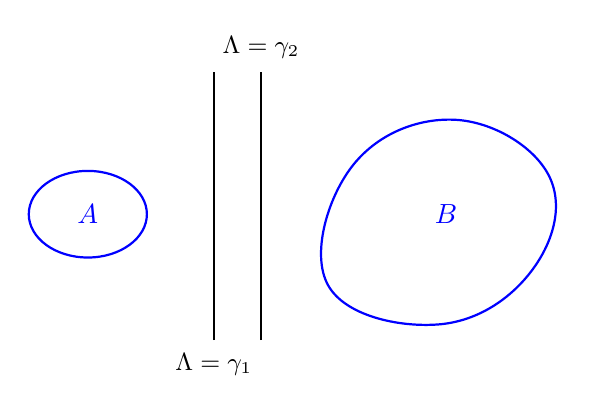
\begin{tikzpicture}[scale=1.0]
	% compact convex A, on the side where $\re\Lambda$ is small
	\draw[thick, color=blue] (0.85,0.9) ellipse (0.75 and 0.55);
	\node[color=blue] at (0.85,0.9) {$A$};
	% separating hyperplanes
	\draw[thick] (2.45,-0.7) -- (2.45,2.7);
	\draw[thick] (3.05,-0.7) -- (3.05,2.7);
	\node[below] at (2.45,-0.75) {\small $\re \Lambda = \gamma_1$};
	\node[above] at (3.05,2.75) {\small $\re \Lambda = \gamma_2$};
	% closed convex set B
	\begin{scope}[xshift=3.9cm]
		\draw[thick, color=blue] plot[smooth cycle, tension=0.7] coordinates
			{(0,0) (1.4,-0.5) (2.6,0.2) (2.8,1.4) (1.6,2.1) (0.3,1.5)};
		\node[color=blue] at (1.5,0.9) {$B$};
	\end{scope}
\end{tikzpicture}
\end{center}

\begin{corollary}\label{cor:hbsep}
	For distinct $x,y$ in a normed space $X$ there is $\Lambda \in X'$ with $\Lambda(x) \ne \Lambda(y)$.
\end{corollary}

\begin{proof}
	Apply Theorem \ref{thm:geomhb}(b) with $A = \{x\}$ and $B = \{y\}$ (or Corollary \ref{cor:hbnormattained} to $x - y$).
\end{proof}

\begin{corollary}\label{cor:hbdense}
	Let $M \le X$ be a subspace with $\ol M \ne X$, and let $x_0 \in X \setminus \ol M$. Then there is $\Lambda \in X'$ with $\Lambda(x_0) = 1$ and $\Lambda|_M = 0$.
\end{corollary}

\begin{proof}
	Take $A = \{x_0\}$, $B = \ol M$ in Theorem \ref{thm:geomhb}(b) to get $\Lambda_0$ with $\re \Lambda_0(x_0) < \gamma_1 < \gamma_2 < \re\Lambda_0(y)$ for $y \in \ol M$. Since $\ol M$ is a subspace, $\Lambda_0(\ol M)$ is a subspace of $\F$ bounded away from $\re\Lambda_0(x_0)$, which forces $\Lambda_0|_M = 0$; then rescale.
\end{proof}

\begin{remark}
	Corollary \ref{cor:hbdense} is the standard tool for proving \emph{density}: to show a subspace $M$ is dense in $X$, it suffices to show that the only $\Lambda \in X'$ vanishing on $M$ is $\Lambda = 0$. This is usually much easier, because we have a concrete description of $X'$ to work with. We shall use exactly this manoeuvre when studying Sobolev spaces.
\end{remark}

\subsection{Consequences of Baire category}

We record, without proof, three theorems from Linear Analysis which all follow from the Baire category theorem (a complete metric space is not a countable union of nowhere dense sets). Their common feature is that they turn a pointwise or algebraic hypothesis into a uniform or topological conclusion. Proofs of all three, and of Baire's theorem itself, are in my Linear Analysis notes; the same is true of the Hilbert space material of Section \ref{sec:duality} and of the spectral theorem for compact self-adjoint operators, which we shall borrow in Section \ref{sec:pde}.

\begin{theorem}[Principle of uniform boundedness]\label{thm:ubp}
	Let $X$ be a Banach space, $Y$ a normed space, and $\mathcal{T} \subseteq \mathcal{B}(X,Y)$ a family of bounded operators with $\sup_{T \in \mathcal{T}}\norm{Tx} < \infty$ for every $x \in X$. Then $\sup_{T\in\mathcal{T}}\norm{T} < \infty$.
\end{theorem}

\begin{theorem}[Open mapping theorem]\label{thm:omt}
	A surjective bounded linear map between Banach spaces is open. In particular a bijective bounded linear map has bounded inverse.
\end{theorem}

\begin{theorem}[Closed graph theorem]\label{thm:cgt}
	A linear map between Banach spaces whose graph is closed is bounded.
\end{theorem}

The consequence we need immediately is the following, which says that weak convergence -- defined in a moment -- cannot produce unbounded sequences.

\begin{proposition}\label{prop:weakbounded}
	Let $X$ be a Banach space and $(x_n)$ a sequence with $\Lambda(x_n)$ convergent for every $\Lambda \in X'$. Then $(\norm{x_n})$ is bounded.
\end{proposition}

\begin{proof}
	View each $x_n$ as an element $f_{x_n}$ of $X'' = \mathcal{B}(X', \F)$, noting $X'$ is a Banach space. For each $\Lambda$ the sequence $f_{x_n}(\Lambda) = \Lambda(x_n)$ is convergent, hence bounded. By Theorem \ref{thm:ubp}, $\sup_n \norm{f_{x_n}}_{X''} < \infty$; and $\norm{f_{x_n}}_{X''} = \norm{x_n}$ by Corollary \ref{cor:hbnormattained}.
\end{proof}

\subsection{Seminorms and locally convex spaces}

To define the weak topologies properly we need topologies generated not by a norm but by a family of seminorms.

\begin{definition}[Seminorm]
	A \vocab{seminorm} on a vector space $X$ over $\F$ is a map $p : X \to \R$ with $p(x+y)\le p(x)+p(y)$ and $p(\lambda x) = |\lambda| p(x)$.
\end{definition}

Taking $\lambda = 0$ gives $p(0) = 0$, and then $0 = p(0) \le 2p(x)$ shows $p \ge 0$. So a seminorm is a norm except that $p(x) = 0$ need not force $x = 0$. A single seminorm is therefore too coarse to separate points; the idea is to use many of them.

\begin{definition}
	A family $\mathcal{P}$ of seminorms on $X$ is \vocab{separating} if for every $x \ne 0$ there is $p \in \mathcal{P}$ with $p(x) \ne 0$.
\end{definition}

Given a separating family $\mathcal{P}$, set $V(p,n) = \{x : p(x) < 1/n\}$ for $p \in \mathcal{P}$ and $n \in \N$, let $\dot\beta$ be the collection of finite intersections of such sets, and let $\beta = \{x + B : x \in X, B \in \dot\beta\}$.

\begin{theorem}\label{thm:lctvs}
	$\beta$ is a base for a Hausdorff topology $\tau_{\mathcal{P}}$ on $X$, with respect to which addition, scalar multiplication and every $p \in \mathcal{P}$ are continuous.
\end{theorem}

\begin{definition}
	A space of the form $(X, \tau_\mathcal{P})$ is a \vocab{locally convex topological vector space}, or LCTVS. If $\mathcal{P} = \{p_n\}_{n \in \N}$ is countable, $\tau_\mathcal{P}$ is metrisable by
	$$d(x,y) = \sum_{n=1}^\infty 2^{-n} \frac{p_n(x-y)}{1 + p_n(x-y)},$$
	and if this metric is complete we call $X$ a \vocab{Fr\'echet space}.
\end{definition}

`Locally convex' refers to the fact that the basic neighbourhoods $V(p,n)$ are convex, which is exactly the hypothesis needed for Hahn--Banach separation arguments to work. All the spaces in this course are locally convex; we shall meet Fr\'echet spaces again when we build test functions.

\subsection{Weak and weak-\texorpdfstring{$*$}{*} topologies}

Let $X$ be a Banach space. Taking $\mathcal{P} = \{\norm{\cdot}\}$ recovers the norm topology, which for contrast we now call the \vocab{strong topology} $\tau_s$; convergence in it, written $x_n \to x$, means $\norm{x_n - x}\to 0$.

\begin{definition}[Weak topology]
	For $\Lambda \in X'$ the map $p_\Lambda(x) = |\Lambda(x)|$ is a seminorm, and the family $\{p_\Lambda : \Lambda \in X'\}$ is separating by Corollary \ref{cor:hbsep}. The topology it generates is the \vocab{weak topology} $\tau_w$ on $X$. Thus $x_n \weakto x$ (`$x_n$ converges weakly to $x$') if and only if
	$$\Lambda(x_n) \to \Lambda(x) \quad \text{for all } \Lambda \in X'.$$
\end{definition}

\begin{definition}[Weak-$*$ topology]
	The dual $X'$ carries its own strong and weak topologies, but also a third: the family of seminorms $\{p_x : \Lambda \mapsto |\Lambda(x)| \, : \, x \in X\}$ generates the \vocab{weak-$*$ topology} $\tau_{w*}$ on $X'$. Thus $\Lambda_n \wsto \Lambda$ if and only if $\Lambda_n(x) \to \Lambda(x)$ for every $x \in X$: weak-$*$ convergence is pointwise convergence of functionals.
\end{definition}

Since $X \subseteq X''$, the weak-$*$ topology on $X'$ is coarser than its weak topology, and the two coincide exactly when $X$ is reflexive. Strong convergence implies weak convergence implies weak-$*$ convergence, and none of the implications reverses.

\begin{example}\label{ex:weaknotstrong}
	Two examples of weak convergence to $0$ without strong convergence, which between them illustrate the two mechanisms available.
	\begin{enumerate}[label=(\roman*)]
		\item (\emph{Oscillation.}) In $L^2((0,2\pi))$ let $f_n(x) = \sin(nx)$. Then $\norm{f_n}_{L^2} = \sqrt\pi$ for all $n$, so $f_n \not\to 0$ strongly. But $\int_0^{2\pi} g(x)\sin(nx) \dd x \to 0$ for every $g \in L^2$: this is true for $g$ in the dense set of trigonometric polynomials by orthogonality, hence for all $g$ by density and uniform boundedness. So $f_n \weakto 0$. The mass does not go away; it is redistributed into ever higher frequencies, and every fixed test function averages it out.
		\item (\emph{Escape to infinity.}) In $L^2(\R)$ let $g_n(x) = \phi(x - n)$ for a fixed non-zero bump $\phi$. Again $\norm{g_n}_{L^2} = \norm{\phi}_{L^2}$ is constant, but for $h \in C_c(\R)$ the supports eventually separate, so $\int h g_n = 0$ for large $n$, and density gives $g_n \weakto 0$. The mass is neither destroyed nor spread out -- it simply escapes to infinity.
	\end{enumerate}
\begin{center}
\begin{tikzpicture}[scale=1.0]
	\begin{scope}
		\draw[<->] (-0.3,0) -- (6.9,0);
		\draw[<->] (0,-1.5) -- (0,1.5);
		\draw[thick, color=gray] plot[domain=0:6.283,samples=120,smooth] (\x, {sin(\x r)});
		\draw[thick, color=blue] plot[domain=0:6.283,samples=400] (\x, {sin(8*\x r)});
		\node[color=gray] at (1.75,1.25) {\small $f_1$};
		\node[color=blue] at (5.4,1.25) {\small $f_8$};
	\end{scope}
	\begin{scope}[yshift=-3.6cm]
		\draw[<->] (-0.3,0) -- (6.9,0);
		\draw[<->] (0,-0.4) -- (0,1.5);
		\foreach \s/\c in {1/gray, 3/gray, 5/blue} {
			\begin{scope}[xshift=\s cm, yscale=1.0, xscale=0.55]
				\draw[thick, color=\c] \bumppath;
			\end{scope}
		}
		\node[color=gray] at (1,1.25) {\small $g_1$};
		\node[color=gray] at (3,1.25) {\small $g_3$};
		\node[color=blue] at (5,1.25) {\small $g_5$};
	\end{scope}
\end{tikzpicture}
\end{center}
\end{example}

\begin{example}
	Specialising to our spaces: for $1 \le p < \infty$ and $f_i, f \in L^p(\R^n)$, we have $f_i \weakto f$ if and only if
	$$\int_{\R^n} g f_i \longrightarrow \int_{\R^n} gf \quad \text{for all } g \in L^q(\R^n),$$
	by Theorem \ref{thm:lpdual}. When $1 < p < \infty$ the space is reflexive and this is the same as weak-$*$ convergence. For $f_i \in L^\infty(\R^n) = L^1(\R^n)'$, weak-$*$ convergence means testing against all $g \in L^1$, which is strictly weaker than weak convergence, since $(L^\infty)'$ is strictly bigger than $L^1$.
\end{example}

Oscillation is by far the more common of the two mechanisms, and it is worth having a general statement. The following says that a rapidly oscillating periodic function converges weakly to its mean -- the oscillations are not damped, they are simply averaged out by any fixed test function.

\begin{proposition}[Oscillating sequences]\label{prop:oscillation}
	Let $g \in L^\infty(\R)$ be $1$-periodic with mean $\ol g = \int_0^1 g(t)\dd t$, and set $g_m(x) = g(mx)$. Then $g_m \wsto \ol g$ in $L^\infty(\R) = L^1(\R)'$; that is,
	$$\int_\R h(x)g(mx)\dd x \longrightarrow \ol g \int_\R h(x) \dd x \quad \text{for every } h \in L^1(\R).$$
\end{proposition}

\begin{proof}
	Each $g_m$ has $\norm{g_m}_{L^\infty}=\norm{g}_{L^\infty}$, so the functionals $\Lambda_m(h)=\int hg_m$ have uniformly bounded norms on $L^1(\R)$. A uniformly bounded family of functionals which converges on a dense subset converges everywhere: if $\norm{\Lambda_m}\le C$ and $\Lambda_m(h_0)$ converges for $h_0$ in a dense set, then for general $h$ and $\varepsilon>0$ we may pick $h_0$ with $\norm{h-h_0}_{L^1}<\varepsilon$ and estimate $|\Lambda_m(h)-\Lambda_{m'}(h)|\le 2C\varepsilon+|\Lambda_m(h_0)-\Lambda_{m'}(h_0)|$, so $(\Lambda_m(h))$ is Cauchy.

	So it is enough to treat $h = \ii_{[a,b]}$, since finite linear combinations of such indicators are dense in $L^1(\R)$. Substituting $t = mx$,
	$$\int_a^b g(mx)\dd x = \frac 1m \int_{ma}^{mb}g(t)\dd t.$$
	The interval $[ma,mb]$ has length $m(b-a)$ and so contains $N_m = \lfloor m(b-a)\rfloor$ complete periods of $g$, each contributing $\ol g$, together with a leftover interval of length at most $1$ on which the integral is at most $\norm{g}_{L^\infty}$ in modulus. Hence
	$$\left| \frac 1m\int_{ma}^{mb}g - \frac{N_m}{m}\ol g\right| \le \frac{\norm{g}_{L^\infty}}{m} \longrightarrow 0,$$
	and $N_m/m \to b-a$, giving the claim.
\end{proof}

\begin{example}\label{ex:squarestrick}
	Take $g(x)=\sin(2\pi x)$, so $\ol g = 0$ and $u_m(x) = \sin(2\pi mx)\wsto 0$. But now consider $u_m^2 = \sin^2(2\pi m x)$: this is again of the form $G(mx)$ for the $1$-periodic $G = \sin^2(2\pi\, \cdot)$, whose mean is $1/2$, so
	$$u_m \wsto 0 \quad \text{while} \quad u_m^2 \wsto \tfrac12 \ne 0 = \left( \text{weak limit of } u_m\right)^2.$$
	This little computation deserves to be remembered, because it is the whole difficulty of the last third of the course in miniature. Weak limits do not commute with nonlinear operations. Any functional built by integrating a nonlinear function of $u$ will therefore fail to be weakly \emph{continuous}, and the best we can hope for is an inequality in one direction. Note which direction we got here: $\frac 12 > 0$, so the limit of $\int u_m^2$ is \emph{larger} than $\int u^2$. That is lower semicontinuity, and Section \ref{sec:direct} explains why convexity of the integrand always makes it fall this way.
\end{example}

\begin{remark}
	Two warnings. First, the weak topology is \emph{not} metrisable on an infinite-dimensional space (though it is metrisable on bounded sets when $X'$ is separable), so one must be careful with sequential arguments; we shall always be in the situation where sequences suffice. Second, weak convergence is strictly weaker than strong convergence, but by Proposition \ref{prop:weakbounded} a weakly convergent sequence is still bounded, and one always has
	$$\norm{x} \le \liminf_{n\to\infty}\norm{x_n} \quad \text{when } x_n \weakto x,$$
	since $\norm{x} = \sup_{\norm{\Lambda}\le 1}|\Lambda(x)| = \sup_\Lambda \lim_n |\Lambda(x_n)| \le \liminf_n \norm{x_n}$. The norm can drop in the limit -- it did in both parts of Example \ref{ex:weaknotstrong}, from a positive constant to $0$ -- but it cannot jump up. This inequality, \vocab{weak lower semicontinuity of the norm}, is the single most useful property of weak convergence, and everything in Section \ref{sec:direct} is built on it.
\end{remark}

\subsection{Banach--Alaoglu}

Now the pay-off. It is worth recalling first the one compactness theorem for function spaces that we already have, from the topology of $C(K)$: it buys strong (uniform) convergence, but at the price of a hypothesis -- equicontinuity -- that is much too strong to verify in practice.

\begin{theorem}[Arzel\`a--Ascoli, a weak form]\label{thm:arzela}
	Let $(f_i)$ be a sequence of functions $[0,1]\to\C$ which is bounded and equicontinuous. Then $(f_i)$ has a uniformly convergent subsequence.
\end{theorem}

What follows is the trade we advertised: we drop equicontinuity entirely, keep only boundedness, and accept a much weaker form of convergence in exchange.

\begin{theorem}[Banach--Alaoglu]\label{thm:alaoglu}
	Let $X$ be a normed space and $\ol{B}' = \{\Lambda \in X' : \norm{\Lambda}_{X'}\le 1\}$ the closed unit ball of the dual. Then $\ol{B}'$ is compact in the weak-$*$ topology.
\end{theorem}

The general statement is proved by embedding $\ol B'$ into the product $\prod_{x \in X}\{z : |z| \le \norm{x}\}$ and applying Tychonoff's theorem, and therefore uses the axiom of choice in an essential way. For our purposes a sequential version on separable spaces is enough, and it can be proved by hand with a diagonal argument.

\begin{theorem}[Banach--Alaoglu, sequential form]\label{thm:alaoglu2}
	Let $X$ be a separable Banach space and let $(\Lambda_j)_{j=1}^\infty$ be a sequence in $\ol B' \subseteq X'$. Then there is a subsequence $(\Lambda_{j_k})$ and $\Lambda \in \ol B'$ with $\Lambda_{j_k}\wsto\Lambda$.
\end{theorem}

\begin{proof}
	Let $D = \{x_1, x_2, \dots\}$ be a countable dense subset of $X$.

	\emph{Diagonal extraction.} The sequence $(\Lambda_j(x_1))_j$ is bounded in $\F$, since $|\Lambda_j(x_1)| \le \norm{x_1}$. By Bolzano--Weierstrass some subsequence converges, to a limit we call $\Lambda(x_1)$; write $\Lambda_{1,k}$ for this subsequence. Extract from it a further subsequence $\Lambda_{2,k}$ along which $\Lambda_{2,k}(x_2)$ converges, to $\Lambda(x_2)$; and so on. The diagonal sequence $\Lambda_{j,j}$ is eventually a subsequence of each $\Lambda_{l,k}$, so $\Lambda_{j,j}(x) \to \Lambda(x)$ for every $x \in D$, with $|\Lambda(x)| \le \norm{x}$.

	\emph{Extension to $X$.} The map $\Lambda : D \to \F$ is Lipschitz: given $x, y \in D$, choose $k$ so large that $|\Lambda_{k,k}(x)-\Lambda(x)|$ and $|\Lambda_{k,k}(y)-\Lambda(y)|$ are both less than $\varepsilon$; then
	$$|\Lambda(x)-\Lambda(y)| \le |\Lambda(x)-\Lambda_{k,k}(x)| + |\Lambda_{k,k}(x-y)| + |\Lambda_{k,k}(y)-\Lambda(y)| \le 2\varepsilon + \norm{x-y}.$$
	As $\varepsilon$ was arbitrary, $\Lambda$ is $1$-Lipschitz on $D$ and so extends uniquely to a continuous map on $X = \ol D$.

	\emph{Linearity.} Let $x, y \in X$ and $a \in \F$, and set $z = x + ay$. Choose $x', y', z' \in D$ close to $x, y, z$ respectively with $z' = x' + ay'$ approximately; then
	\begin{align*}
		|\Lambda(z) - \Lambda(x)-a\Lambda(y)| &\le |\Lambda(z)-\Lambda(z')| + |\Lambda(x)-\Lambda(x')| + |a| |\Lambda(y)-\Lambda(y')| \\
		&\quad + |\Lambda(z')-\Lambda_{k,k}(z')| + |\Lambda(x')-\Lambda_{k,k}(x')| \\
		&\quad + |a| |\Lambda(y')-\Lambda_{k,k}(y')| \\
		&\quad + |\Lambda_{k,k}(z'-x'-ay')|,
	\end{align*}
	and each line is small: the first by continuity of $\Lambda$ and the choice of $x',y',z'$, the second by taking $k$ large, the third because $\Lambda_{k,k}$ is linear of norm at most $1$ and $z'-x'-ay'$ is small. So $\Lambda$ is linear, and being $1$-Lipschitz, $\Lambda \in \ol B'$.

	\emph{Convergence.} Finally, for arbitrary $x \in X$ pick $x' \in D$ with $\norm{x - x'}$ small; then
	$$|\Lambda_{j,j}(x)-\Lambda(x)| \le |\Lambda_{j,j}(x-x')| + |\Lambda_{j,j}(x')-\Lambda(x')| + |\Lambda(x'-x)|,$$
	where the outer terms are at most $\norm{x-x'}$ each and the middle tends to $0$. Hence $\Lambda_{j,j}\wsto\Lambda$.
\end{proof}

The theorem is worth pausing over. The closed unit ball of $X'$ is never norm-compact in infinite dimensions, and yet it is always weak-$*$ compact. Nothing has been gained for free: what we get in exchange for compactness is that the limit is only a weak-$*$ limit, so that the convergence carries very little information. The whole art of the subject is to use structure -- convexity, an equation, an estimate -- to upgrade the weak limit afterwards.

\begin{center}
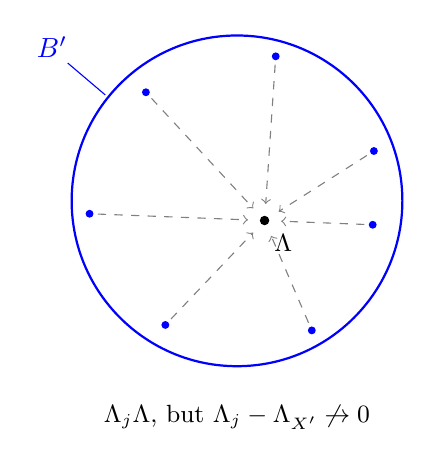
\begin{tikzpicture}[scale=1.0]
	\draw[thick, color=blue] (0,0) circle (2.1);
	\node[color=blue] at (-2.35,1.95) {$\ol B'$};
	\draw[color=blue, shorten >=2pt] (-2.15,1.75) -- (-1.62,1.3);
	% a sequence with no strongly convergent subsequence, but a weak-* limit
	\foreach \a/\r in {20/1.85, 75/1.9, 130/1.8, 185/1.88, 240/1.82, 300/1.9, 350/1.75} {
		\fill[color=blue] (\a:\r) circle (0.05);
	}
	\fill (0.35,-0.25) circle (0.06);
	\node[below right] at (0.35,-0.3) {\small $\Lambda$};
	\foreach \a/\r in {20/1.85, 75/1.9, 130/1.8, 185/1.88, 240/1.82, 300/1.9, 350/1.75} {
		\draw[->, dashed, color=gray, shorten >=6pt, shorten <=3pt] (\a:\r) -- (0.35,-0.25);
	}
	\node at (0,-2.75) {\small $\Lambda_j \wsto \Lambda$, but $\norm{\Lambda_j - \Lambda}_{X'} \not\to 0$};
\end{tikzpicture}
\end{center}

\begin{corollary}\label{cor:weakcompactlp}
	Let $1 < p \le \infty$ and let $(f_j)$ be a sequence in $L^p(\R^n)$ with $\norm{f_j}_{L^p}\le K$ for all $j$. Then there is a subsequence $(f_{j_k})$ and $f \in L^p(\R^n)$ with $\norm{f}_{L^p}\le K$ and
	$$\int_{\R^n} f_{j_k} g \dd x \longrightarrow \int_{\R^n} fg \dd x \quad \text{for all } g \in L^q(\R^n).$$
\end{corollary}

\begin{proof}
	$L^p(\R^n) = L^q(\R^n)'$ by Theorem \ref{thm:lpdual}, and $L^q(\R^n)$ is separable since $q < \infty$ (Proposition \ref{prop:separable}). Apply Theorem \ref{thm:alaoglu2} to $K^{-1}f_j$.
\end{proof}

\begin{corollary}\label{cor:reflexiveweak}
	In a reflexive Banach space $X$ (in particular in any Hilbert space, or in $L^p$ for $1<p<\infty$), every bounded sequence has a weakly convergent subsequence.
\end{corollary}

\begin{proof}
	Apply Theorem \ref{thm:alaoglu2} to the sequence viewed in $X'' = (X')'$, using that weak-$*$ and weak convergence coincide on a reflexive space. (For the separability hypothesis one restricts to the closed span of the sequence, which is a separable reflexive space.)
\end{proof}

Notice that $p=1$ is excluded, and this is not an oversight. In $L^1(\R)$ the sequence $f_n = n \ii_{[0,1/n]}$ is bounded, but it has no weakly convergent subsequence: the only candidate limit is the Dirac mass at $0$, which is not a function. Failures of weak compactness in $L^1$ are always of this type -- concentration -- and controlling them is the subject of the Dunford--Pettis theorem, which we shall not need.

\section{Convexity and the Direct Method}\label{sec:direct}

We now set out, in the abstract, the method by which we shall later prove that partial differential equations have solutions. The idea goes back to Hilbert and is disarmingly simple: to find a minimiser of a functional $S$, take a sequence $u_n$ along which $S[u_n]$ tends to the infimum, extract a convergent subsequence, and hope that the limit is a minimiser. Every step of this can fail, and the interest is entirely in the conditions which make it work.

\subsection{Lower semicontinuity}

\begin{definition}
	Let $X$ be a topological space. A functional $S : X \to \R \cup \{+\infty\}$ is \vocab{(sequentially) lower semicontinuous} if
	$$u_n \to u \implies S[u] \le \liminf_{n\to\infty}S[u_n].$$
	It is \vocab{coercive} if every sublevel set $\{u : S[u] \le K\}$ is sequentially relatively compact -- that is, if $S[u_n]\le K$ for all $n$ then $(u_n)$ has a convergent subsequence.
\end{definition}

Continuity implies lower semicontinuity, but not conversely. The point of the weaker hypothesis is that the value of $S$ is allowed to \emph{drop} in a limit but not to jump up; and dropping is harmless when we are minimising.

\begin{center}
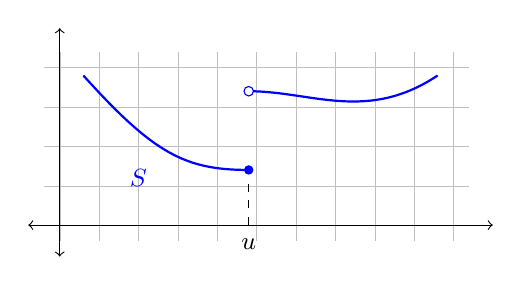
\begin{tikzpicture}[scale=1.0]
	\draw[ultra thin, color=lightgray, step=0.5] (-0.2,-0.2) grid (5.2,2.2);
	\draw[<->] (-0.4,0) -- (5.5,0);
	\draw[<->] (0,-0.4) -- (0,2.5);
	% lower semicontinuous: value at jump is the LOWER one
	\draw[thick, color=blue] (0.3,1.9) .. controls (1.2,0.9) and (1.6,0.7) .. (2.4,0.7);
	\draw[thick, color=blue] (2.4,1.7) .. controls (3.2,1.7) and (3.9,1.3) .. (4.8,1.9);
	\fill[color=blue] (2.4,0.7) circle (0.06);
	\draw[color=blue, fill=white] (2.4,1.7) circle (0.06);
	\node[color=blue] at (1.0,0.6) {\small $S$};
	\draw[dashed] (2.4,0) -- (2.4,0.62);
	\node[below] at (2.4,-0.05) {\small $u$};
\end{tikzpicture}
\end{center}

\begin{theorem}[The direct method]\label{thm:directabstract}
	Let $X$ be a topological space and $S : X \to \R$ coercive and lower semicontinuous. Then $S$ attains its infimum on $X$.
\end{theorem}

\begin{proof}
	Let $\sigma = \inf\{S[u] : u \in X\} \in [-\infty,\infty)$ and choose a \vocab{minimising sequence} $(u_n)$ with $S[u_n]\to\sigma$. In particular $(S[u_n])$ is bounded above, say by $K$, so coercivity provides a subsequence $u_{n_j}\to u^*$ for some $u^*\in X$. By lower semicontinuity,
	$$S[u^*]\le \liminf_{j\to\infty}S[u_{n_j}] = \sigma.$$
	As $S[u^*]\ge\sigma$ by definition of the infimum, we get $S[u^*] = \sigma$; in particular $\sigma > -\infty$.
\end{proof}

That is the entire method, and as stated it is nearly vacuous. All the work lies in verifying the two hypotheses, and here we run into a fundamental tension. Coercivity asks for compactness, which wants a \emph{weak} topology; lower semicontinuity asks for the functional to behave well under limits, which wants a \emph{strong} topology. Any given functional will typically satisfy one and fail the other. Resolving this is the content of the rest of the section, and the resolution is convexity.

\begin{center}
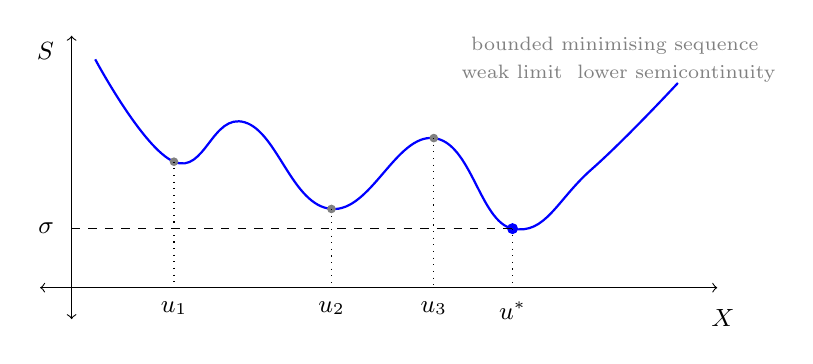
\begin{tikzpicture}[scale=1.0]
	\draw[<->] (-0.4,0) -- (8.2,0);
	\draw[<->] (0,-0.4) -- (0,3.2);
	\node[left] at (-0.1,3.0) {\small $S$};
	\node[below right] at (8.0,-0.15) {\small $X$};
	% a "landscape"
	\draw[thick, color=blue] plot[smooth, tension=0.75] coordinates
		{(0.3,2.9) (1.3,1.6) (2.2,2.1) (3.3,1.0) (4.6,1.9) (5.6,0.75) (6.6,1.5) (7.7,2.6)};
	% minimising sequence
	\foreach \x/\y in {1.3/1.6, 3.3/1.0, 4.6/1.9} { \fill[color=gray] (\x,\y) circle (0.055); }
	\fill[color=blue] (5.6,0.75) circle (0.07);
	\draw[dashed] (0,0.75) -- (5.6,0.75);
	\node[left] at (-0.1,0.75) {\small $\sigma$};
	\node[below] at (1.3,-0.05) {\small $u_1$};
	\node[below] at (3.3,-0.05) {\small $u_2$};
	\node[below] at (4.6,-0.05) {\small $u_3$};
	\node[below] at (5.6,-0.05) {\small $u^*$};
	\draw[dotted] (1.3,1.6) -- (1.3,0); \draw[dotted] (3.3,1.0) -- (3.3,0);
	\draw[dotted] (4.6,1.9) -- (4.6,0); \draw[dotted] (5.6,0.75) -- (5.6,0);
	\node[align=center, color=gray] at (6.9,2.9) {\scriptsize bounded minimising sequence \\[-2pt] \scriptsize $\rightsquigarrow$ weak limit $\rightsquigarrow$ lower semicontinuity};
\end{tikzpicture}
\end{center}

\subsection{Coercivity in the weak topology}

From now on let $X$ be a reflexive separable Banach space. On such a space, coercivity in the weak topology is nothing more than an a priori bound.

\begin{lemma}\label{lem:weakcoercive}
	Let $X$ be reflexive and suppose $S : X \to \R$ has the property that $S[u]\le K$ implies $\norm{u}\le \wt K$ for some $\wt K$ depending only on $K$. Then $S$ is coercive for the weak topology of $X$.
\end{lemma}

\begin{proof}
	Immediate from Corollary \ref{cor:reflexiveweak}: a bounded sequence has a weakly convergent subsequence.
\end{proof}

So on a reflexive space, coercivity is free -- it is just the statement that sublevel sets of $S$ are bounded, which for a concrete functional is a routine estimate. The difficulty has been entirely displaced onto lower semicontinuity, which we must now verify for the weak topology. Since weak convergence is a much weaker hypothesis on $(u_n)$, weak lower semicontinuity is a much stronger conclusion, and it is simply false in general. (Consider $S[u] = -\norm{u}^2$ on a Hilbert space and $u_n = e_n$: then $u_n \weakto 0$ but $S[u_n] = -1 < 0 = S[0]$.)

\subsection{Convexity saves the day}

\begin{lemma}[Mazur]\label{lem:mazur}
	Let $X$ be a Banach space and $U \subseteq X$ convex and strongly closed. Then $U$ is weakly closed.
\end{lemma}

\begin{proof}
	Let $x \in U^c$. Applying Theorem \ref{thm:geomhb}(b) to the compact convex set $\{x\}$ and the closed convex set $U$ gives $\Lambda \in X'$ and $\gamma_1 < \gamma_2$ with $\re\Lambda(x) < \gamma_1 < \gamma_2 < \re \Lambda(y)$ for all $y \in U$. The set $\{z : \re \Lambda(z) < \gamma_1\}$ is weakly open (it is a preimage of an open set under a weakly continuous map), contains $x$, and is disjoint from $U$. So $U^c$ is weakly open.
\end{proof}

The reader should appreciate how much this says. A strongly closed set need not be weakly closed -- the unit \emph{sphere} of a Hilbert space is strongly closed but its weak closure is the whole closed unit ball, since $e_n \weakto 0$. Convexity rules out exactly this kind of behaviour.

\begin{theorem}\label{thm:convexweaklsc}
	Let $X$ be a Banach space and $S : X \to \R$ convex and lower semicontinuous for the strong topology. Then $S$ is lower semicontinuous for the weak topology.
\end{theorem}

\begin{proof}
	For each $K \in \R$ the sublevel set $E_K = \{u : S[u]\le K\}$ is convex (by convexity of $S$) and strongly closed (by strong lower semicontinuity), hence weakly closed by Lemma \ref{lem:mazur}.

	Now suppose $u_n \weakto u^*$, and set $\ell = \liminf_n S[u_n]$; we may assume $\ell < \infty$. Passing to a subsequence we may assume $S[u_{n_j}]\to \ell$. Given $\varepsilon > 0$, there is $J$ with $S[u_{n_j}]\le \ell + \varepsilon$ for $j \ge J$, i.e.\ $u_{n_j}\in E_{\ell + \varepsilon}$ for $j \ge J$. Since $E_{\ell+\varepsilon}$ is weakly closed and $u_{n_j}\weakto u^*$, we get $u^* \in E_{\ell+\varepsilon}$, that is $S[u^*]\le\ell+\varepsilon$. As $\varepsilon > 0$ was arbitrary, $S[u^*]\le\ell$.
\end{proof}

Putting the pieces together we obtain the theorem we shall use.

\begin{corollary}\label{cor:directconvex}
	Let $X$ be a reflexive Banach space and $S : X \to \R$ convex, strongly lower semicontinuous, and with bounded sublevel sets. Then $S$ attains its infimum on $X$.
\end{corollary}

\begin{proof}
	Combine Lemma \ref{lem:weakcoercive}, Theorem \ref{thm:convexweaklsc} and Theorem \ref{thm:directabstract}, all applied to the weak topology. (Strictly, Theorem \ref{thm:directabstract} was stated for sequential compactness and sequential lower semicontinuity, which is exactly what the three results provide.)
\end{proof}

\begin{example}
	The norm itself is convex and continuous, so $u \mapsto \norm{u}$ is weakly lower semicontinuous: this recovers the inequality $\norm{u^*}\le\liminf\norm{u_n}$ for $u_n \weakto u^*$ that we saw directly earlier. More usefully, so is $u \mapsto \norm{u}^2 - 2\re\Lambda(u)$ for a fixed $\Lambda \in X'$, and this functional has bounded sublevel sets since
	$$\norm{u}^2 - 2\re\Lambda(u) \ge \norm{u}^2 - 2\norm{\Lambda}\norm{u} \to \infty$$
	as $\norm{u}\to\infty$. So it attains its infimum. In a Hilbert space this is a long-winded proof of the Riesz representation theorem; on a Sobolev space it will be a proof that the Dirichlet problem has a solution.
\end{example}

Convexity is not a technical convenience that a cleverer argument might remove. Here is the standard example showing that without it the conclusion is simply false.

\begin{example}[Bolza]\label{ex:bolza}
	Work on $X = H_0^1((0,1))$ -- a space we shall construct properly in Section \ref{sec:sobolev}, but for now the reader may think of piecewise smooth functions on $[0,1]$ vanishing at the endpoints. Define
	$$S[u]=\int_0^1\left( \left(u'(x)^2-1\right)^2+u(x)^2\right)\dd x.$$
	Clearly $S \ge 0$. I claim $\inf S = 0$, but that no $u$ attains it.

	That the infimum is not attained is easy: $S[u]=0$ would force $u = 0$ almost everywhere, hence $u' = 0$ almost everywhere, and then the first term of the integrand equals $1$ everywhere, so $S[u]=1$. Contradiction.

	That the infimum is nevertheless $0$ is the interesting half. Let $u_m$ be the sawtooth with $m$ teeth: $u_m(0)=0$ and $u_m'=\pm1$, alternating in sign on the $2m$ intervals $[j/(2m),(j+1)/(2m)]$. Then $u_m'(x)^2= 1$ everywhere except at the finitely many corners, so the first term of the integrand vanishes identically, while $0 \le u_m \le 1/(2m)$ pointwise, so
	$$S[u_m]=\int_0^1u_m^2\dd x\le\frac{1}{4m^2}\longrightarrow 0.$$
\begin{center}
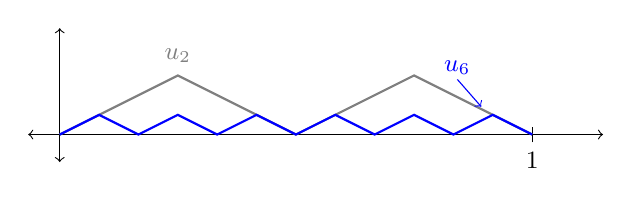
\begin{tikzpicture}[scale=1.0]
	\draw[<->] (-0.4,0) -- (6.9,0);
	\draw[<->] (0,-0.35) -- (0,1.35);
	\draw (6.0,-0.1) -- (6.0,0.1);
	\node[below] at (6.0,-0.1) {\small $1$};
	% u_2 : 2 teeth, peak 1/4 (drawn at 3cm per unit)
	\draw[thick, color=gray] (0,0) -- (1.5,0.75) -- (3,0) -- (4.5,0.75) -- (6,0);
	\node[color=gray] at (1.5,1.0) {\small $u_2$};
	% u_6 : 6 teeth, peak 1/12
	\draw[thick, color=blue] (0,0) -- (0.5,0.25) -- (1,0) -- (1.5,0.25) -- (2,0)
		-- (2.5,0.25) -- (3,0) -- (3.5,0.25) -- (4,0) -- (4.5,0.25) -- (5,0)
		-- (5.5,0.25) -- (6,0);
	\node[color=blue] at (5.05,0.85) {\small $u_6$};
	\draw[color=blue, ->, shorten >=2pt] (5.05,0.7) -- (5.4,0.3);
\end{tikzpicture}
\end{center}
	The minimising sequence oscillates faster and faster; by Proposition \ref{prop:oscillation} it converges weakly (indeed uniformly) to $0$, and $S[0]=1 > 0 = \lim S[u_m]$. So $S$ is \emph{not} weakly lower semicontinuous, and the direct method breaks at exactly the step Theorem \ref{thm:convexweaklsc} was designed to supply. The culprit is visible in the integrand: $z \mapsto (z^2-1)^2$ has two wells and is not convex, so the gradient prefers to spend its time at the two values $\pm 1$ rather than at their average $0$.
\end{example}

\begin{remark}
	It is worth isolating the shape of the argument, because it recurs in every application. To minimise $S$ over $X$:
	\begin{enumerate}[label=(\roman*)]
		\item show $S$ is bounded below and take a minimising sequence $(u_n)$;
		\item derive an a priori bound $\norm{u_n}\le K$ from $S[u_n]\le \sigma + 1$ -- this is a \emph{coercivity} estimate and is where the structure of $S$ enters;
		\item extract $u_{n_j}\weakto u^*$ by reflexivity;
		\item show $S[u^*]\le\liminf S[u_{n_j}]$ using convexity;
		\item conclude that $u^*$ is a minimiser, and derive its Euler--Lagrange equation by differentiating $t \mapsto S[u^*+tv]$ at $t=0$.
	\end{enumerate}
	Step (v) is what connects minimisation to differential equations, and we carry it out in Section \ref{sec:pde}.
\end{remark}

\section{The Fourier Transform}\label{sec:fourier}

The Fourier transform converts differentiation into multiplication, and so turns a differential equation with constant coefficients into algebra. That single fact is worth a whole course. What we want here is a clean account in the language we have built: on which spaces is the transform defined, what are its mapping properties, and can it be inverted.

\subsection{The transform on \texorpdfstring{$L^1$}{L1}}

\begin{definition}[Fourier transform]
	For $f \in L^1(\R^n)$ we define $\FF f = \hat f : \R^n \to \C$ by
	$$\hat f (\xi) = \int_{\R^n} f(x) e^{-i (x\cdot\xi)}\dd x.$$
\end{definition}

Since $|f(x)e^{-i(x\cdot\xi)}| = |f(x)| \in L^1$, the integral converges absolutely for every $\xi$, and $\norm{\hat f}_{L^\infty}\le \norm{f}_{L^1}$. (There are several conventions in circulation, differing by factors of $2\pi$ in the exponent or in front of the integral. We use this one; it makes the differentiation rule clean at the cost of a constant $(2\pi)^n$ in the inversion formula.)

\begin{lemma}[Riemann--Lebesgue]\label{lem:riemannlebesgue}
	Let $f \in L^1(\R^n)$. Then $\hat f \in C^0(\R^n)$ with $\norm{\hat f}_{L^\infty}\le\norm{f}_{L^1}$, and $\hat f(\xi)\to 0$ as $|\xi|\to\infty$.
\end{lemma}

\begin{proof}
	If $\xi_m \to \xi$ then $f(x)e^{-i(x\cdot\xi_m)}\to f(x)e^{-i(x\cdot\xi)}$ pointwise, dominated by $|f| \in L^1$, so $\hat f(\xi_m)\to\hat f(\xi)$ by dominated convergence; and the sup bound is immediate. For the decay, let $\varepsilon > 0$ and use Corollary \ref{cor:ccinftydense} to find $f_\varepsilon \in C_c^\infty(\R^n)$ with $\norm{f - f_\varepsilon}_{L^1}<\varepsilon$. Integrating by parts (there are no boundary terms, as $f_\varepsilon$ has compact support),
	$$\hat f_\varepsilon(\xi) = \int_{\R^n} f_\varepsilon(x) \operatorname{div}_x\!\left( \frac{\xi}{-i|\xi|^2}e^{-i(x\cdot\xi)}\right) \dd x = \int_{\R^n}\frac{\xi \cdot Df_\varepsilon(x)}{i|\xi|^2}e^{-i(x\cdot\xi)}\dd x,$$
	so that $|\hat f_\varepsilon(\xi)|\le |\xi|^{-1}\norm{Df_\varepsilon}_{L^1} < \varepsilon$ once $|\xi|$ is large enough. Then $|\hat f(\xi)|\le|\hat f - \hat f_\varepsilon|+|\hat f_\varepsilon| < 2\varepsilon$ for such $\xi$.
\end{proof}

So $\FF$ maps $L^1(\R^n)$ into the space $C_0(\R^n)$ of continuous functions vanishing at infinity. It is not onto -- the image is a dense proper subspace -- and this is one reason $L^1$ is not the natural home for the transform.

\begin{example}\label{ex:fouriereg}
	Take $n = 1$.
	\begin{enumerate}[label=(\roman*)]
		\item $f = \ii_{(-1,1)}$ has $\hat f(\xi) = \int_{-1}^1 e^{-ix\xi}\dd x = \dfrac{2\sin\xi}{\xi}$ for $\xi \ne 0$, and $\hat f(0)=2$.
		\item $f(x) = e^{-|x|}$ has $\hat f(\xi) = \dfrac{2}{1+\xi^2}$.
		\item $f(x) = \dfrac{1}{1+x^2}$ has $\hat f(\xi) = \pi e^{-|\xi|}$ -- the transform of (ii), up to constants, which is the inversion theorem at work.
		\item $f(x) = e^{-x^2/2}$ has $\hat f(\xi)=\sqrt{2\pi}e^{-\xi^2/2}$. To see this, note $f' = -xf$, so by Theorem \ref{thm:ftderiv} below $i\xi \hat f = -(\hat f)'\cdot(-1)^{-1}$, giving $(\hat f)' = -\xi\hat f$; solving this ODE with $\hat f(0) = \int e^{-x^2/2} = \sqrt{2\pi}$ gives the claim. The Gaussian is (up to scaling) the unique fixed point of $\FF$, which is why it appears everywhere in this subject.
	\end{enumerate}
	The first example is worth drawing, since it shows both the smoothing and the delocalisation.
\begin{center}
\begin{tikzpicture}[scale=1.0]
	\begin{scope}
		\draw[<->] (-2.6,0) -- (2.6,0);
		\draw[<->] (0,-0.35) -- (0,1.5);
		\draw[thick, color=blue] (-2.5,0) -- (-1,0);
		\draw[thick, color=blue] (-1,1) -- (1,1);
		\draw[thick, color=blue] (1,0) -- (2.5,0);
		\draw[color=blue] (-1,0) circle (0.055);
		\draw[color=blue] (1,0) circle (0.055);
		\fill[color=blue] (-1,1) circle (0.055);
		\fill[color=blue] (1,1) circle (0.055);
		\node[below] at (1,-0.05) {\small $1$};
		\node[below] at (-1,-0.05) {\small $-1$};
		\node[color=blue] at (1.9,1.05) {\small $f$};
	\end{scope}
	\begin{scope}[yshift=-3.4cm]
		\draw[<->] (-5.9,0) -- (5.9,0);
		\draw[<->] (0,-0.9) -- (0,2.0);
		\begin{scope}[xscale=0.45, yscale=0.85]
			\draw[thick, color=blue] plot coordinates {
			(-12,-0.0894) (-11.5,-0.1529) (-11,-0.1818) (-10.5,-0.1676)
			(-10,-0.1088) (-9.5,-0.0158) (-9,0.0916) (-8.5,0.1879)
			(-8,0.2473) (-7.5,0.2501) (-7,0.1877) (-6.5,0.0662)
			(-6,-0.0931) (-5.5,-0.2565) (-5,-0.3836) (-4.5,-0.4344)
			(-4,-0.3784) (-3.5,-0.2004) (-3,0.0941) (-2.5,0.4788)
			(-2,0.9093) (-1.5,1.3300) (-1,1.6829) (-0.5,1.9177)
			(0,2) (0.5,1.9177) (1,1.6829) (1.5,1.3300) (2,0.9093)
			(2.5,0.4788) (3,0.0941) (3.5,-0.2004) (4,-0.3784)
			(4.5,-0.4344) (5,-0.3836) (5.5,-0.2565) (6,-0.0931)
			(6.5,0.0662) (7,0.1877) (7.5,0.2501) (8,0.2473)
			(8.5,0.1879) (9,0.0916) (9.5,-0.0158) (10,-0.1088)
			(10.5,-0.1676) (11,-0.1818) (11.5,-0.1529) (12,-0.0894)};
		\end{scope}
		\node[color=blue] at (3.4,1.1) {\small $\hat f(\xi) = \dfrac{2\sin\xi}{\xi}$};
	\end{scope}
\end{tikzpicture}
\end{center}
	Note that $\hat f$ is smooth (indeed real-analytic) but decays only like $|\xi|^{-1}$, and in particular is not integrable. Compact support has been traded for smoothness, and vice versa; this trade-off is a theme.
\end{example}

\subsection{Basic properties}

Write $e_y(x) = e^{i(x\cdot y)}$ and recall $\tau_y f(x) = f(x-y)$ and $\check f(x) = f(-x)$.

\begin{lemma}\label{lem:ftbasic}
	Let $f, g \in L^1(\R^n)$, $y \in \R^n$ and $\mu > 0$.
	\begin{enumerate}[label=(\roman*)]
		\item Writing $f_\mu(x) = \mu^{-n}f(\mu^{-1}x)$, we have $\widehat{f_\mu}(\xi) = \hat f(\mu\xi)$.
		\item $\widehat{e_y f} = \tau_y \hat f$ and $\widehat{\tau_y f} = e_{-y}\hat f$.
		\item $f * g \in L^1(\R^n)$ and $\widehat{f*g} = \hat f \hat g$.
	\end{enumerate}
\end{lemma}

\begin{proof}
	(i) and (ii) are changes of variable. For (iii), Tonelli gives $\norm{f*g}_{L^1}\le\norm{f}_{L^1}\norm{g}_{L^1}$, so $f * g \in L^1$, and then by Fubini
	\begin{align*}
		\widehat{f*g}(\xi) &= \int\!\!\int f(y)g(x-y)e^{-i(x\cdot\xi)}\dd y \dd x \\
		&= \int f(y)e^{-i(y\cdot\xi)}\left( \int g(z)e^{-i(z\cdot\xi)}\dd z\right)\dd y = \hat f(\xi)\hat g(\xi). \qedhere
	\end{align*}
\end{proof}

Part (iii) is the reason the Fourier transform is useful for differential equations: it turns the awkward, non-local operation of convolution into pointwise multiplication.

\begin{theorem}\label{thm:ftderiv}
	\begin{enumerate}[label=(\roman*)]
		\item Suppose $f \in C^1(\R^n)$ with $f, D_jf \in L^1(\R^n)$ for each $j$. Then $\widehat{D_jf}(\xi) = i\xi_j \hat f(\xi)$.
		\item Suppose $(1+|x|)f \in L^1(\R^n)$. Then $\hat f \in C^1(\R^n)$ and $D_j \hat f(\xi) = \widehat{-ix_jf}(\xi)$.
	\end{enumerate}
\end{theorem}

\begin{proof}
	(i) Given $\varepsilon > 0$ choose $f_\varepsilon \in C_c^\infty(\R^n)$ with $\norm{f - f_\varepsilon}_{L^1}+\sum_j \norm{D_jf - D_jf_\varepsilon}_{L^1}<\varepsilon$ (mollify and cut off). For compactly supported smooth functions, integration by parts gives
	$$\widehat{D_jf_\varepsilon}(\xi) = \int e^{-i(x\cdot\xi)}D_jf_\varepsilon(x)\dd x = i\xi_j \int e^{-i(x\cdot\xi)}f_\varepsilon(x)\dd x = i\xi_j\hat f_\varepsilon(\xi).$$
	Hence
	$$|\widehat{D_jf}(\xi)-i\xi_j\hat f(\xi)| \le \norm{D_jf - D_jf_\varepsilon}_{L^1}+|\xi|\norm{f-f_\varepsilon}_{L^1}<(1+|\xi|)\varepsilon,$$
	and letting $\varepsilon \to 0$ with $\xi$ fixed gives the identity.

	(ii) By hypothesis $x_jf \in L^1$, so $\widehat{-ix_jf}$ is defined and continuous. For $h \ne 0$,
	$$\frac{\hat f(\xi+he_j)-\hat f(\xi)}{h} = \int f(x)e^{-i(x\cdot\xi)}\frac{e^{-ix_jh}-1}{h}\dd x,$$
	and the integrand converges pointwise to $-ix_jf(x)e^{-i(x\cdot\xi)}$, dominated by $|x_jf(x)| \in L^1$ since $|e^{i\theta}-1| = 2|\sin(\theta/2)|\le|\theta|$. Dominated convergence finishes the proof.
\end{proof}

In words: \emph{decay of $f$ controls smoothness of $\hat f$, and smoothness of $f$ controls decay of $\hat f$}. A space on which both hold to all orders would be mapped to itself by $\FF$, and this is exactly the definition of the next space.

\subsection{The Schwartz space}

\begin{definition}[Schwartz space]
	A function $\varphi \in C^\infty(\R^n)$ is \vocab{rapidly decreasing} if
	$$p_N(\varphi) = \sup_{x \in \R^n, |\alpha|\le N}\left| (1+|x|)^N D^\alpha \varphi(x)\right| < \infty$$
	for every $N \in \N$. The set of such functions is the \vocab{Schwartz space} $\Sch(\R^n)$, and we equip it with the topology generated by the separating family of seminorms $\{p_N : N \in \N\}$.
\end{definition}

Since the family is countable, $\Sch(\R^n)$ is metrisable, and in fact it is complete, so it is a Fr\'echet space. Concretely, $\varphi_j \to 0$ in $\Sch(\R^n)$ if and only if $\sup_x |(1+|x|)^N D^\alpha \varphi_j(x)|\to 0$ for every $N$ and $\alpha$. One may equally use the seminorms $\sup_{|\alpha|,|\beta|\le N}|x^\beta D^\alpha \varphi(x)|$; they generate the same topology.

\begin{example}
	$\varphi(x) = e^{-|x|^2}$ is in $\Sch(\R^n)$, and so is every element of $C_c^\infty(\R^n)$. The function $(1+|x|^2)^{-1001}$ is not, since it fails to decay faster than every polynomial. Thus
	$$C_c^\infty(\R^n)\subsetneq\Sch(\R^n)\subsetneq C^\infty(\R^n),$$
	with each inclusion continuous.
\end{example}

\begin{corollary}\label{cor:fschwartz}
	$\FF$ maps $\Sch(\R^n)$ continuously into itself.
\end{corollary}

\begin{proof}
	First note the elementary bound, for any $f$ with $(1+|x|)^{n+1}f$ bounded,
	$$\norm{f}_{L^1}=\int_{\R^n}\frac{|f|(1+|x|)^{n+1}}{(1+|x|)^{n+1}}\dd x \le C_n \sup_{x}\left( |f(x)|(1+|x|)^{n+1}\right),$$
	where $C_n = \int_{\R^n}(1+|x|)^{-(n+1)}\dd x<\infty$.
	If $\varphi \in \Sch(\R^n)$ then $D^\alpha(x^\beta\varphi) \in L^1(\R^n)$ for all multi-indices, so applying Theorem \ref{thm:ftderiv} repeatedly gives $\left|\widehat{D^\alpha(x^\beta \varphi)}(\xi)\right| = \left|\xi^\alpha D^\beta \hat\varphi(\xi)\right|$ up to signs, whence
	$$\sup_\xi \left| \xi^\alpha D^\beta \hat\varphi(\xi)\right| \le \norm{D^\alpha(x^\beta\varphi)}_{L^1}\le C_{\alpha,\beta}\sup_{x, |\delta|\le|\alpha|}(1+|x|)^{|\beta|+n+1}|D^\delta \varphi(x)|.$$
	The right-hand side is finite, so $\hat\varphi\in\Sch(\R^n)$; and if $\varphi_j \to 0$ in $\Sch$ then the same estimate gives $\hat\varphi_j\to 0$ in $\Sch$, which is continuity.
\end{proof}

\subsection{Inversion}

\begin{theorem}[Fourier inversion]\label{thm:ftinv}
	Suppose $f, \hat f \in L^1(\R^n)$. Then for almost every $x$,
	$$f(x) = \frac{1}{(2\pi)^n}\int_{\R^n}\hat f(\xi)e^{i(x\cdot\xi)}\dd \xi.$$
	If $f$ is in addition continuous, the identity holds for every $x$.
\end{theorem}

\begin{proof}
	The naive computation -- substitute the definition of $\hat f$ and swap the integrals -- fails, because $e^{i((x-y)\cdot\xi)}$ is not integrable in $\xi$. The standard repair is to insert a Gaussian convergence factor.

	Let $G(\xi) = e^{-|\xi|^2/2}$ and recall from Example \ref{ex:fouriereg}(iv) (applied in each variable) that $\hat G = (2\pi)^{n/2}G$. For $\varepsilon > 0$ consider
	$$I_\varepsilon(x) = \frac{1}{(2\pi)^n}\int_{\R^n} \hat f(\xi)G(\varepsilon\xi)e^{i(x\cdot\xi)}\dd\xi.$$
	Since $|\hat f(\xi)G(\varepsilon\xi)|\le|\hat f(\xi)| \in L^1$ and $G(\varepsilon\xi)\to 1$ pointwise, dominated convergence gives $I_\varepsilon(x) \to (2\pi)^{-n}\int \hat f(\xi)e^{i(x\cdot\xi)}\dd\xi$ as $\varepsilon\to 0$, for every $x$.

	On the other hand, everything in sight is now absolutely integrable in $(\xi,y)$ jointly, so Fubini applies:
	$$I_\varepsilon(x) = \frac{1}{(2\pi)^n}\int_{\R^n} f(y)\left( \int_{\R^n}G(\varepsilon\xi)e^{i((x-y)\cdot\xi)}\dd\xi\right)\dd y = \int_{\R^n}f(y)k_\varepsilon(x-y)\dd y,$$
	where, by Lemma \ref{lem:ftbasic}(i) and $\hat G = (2\pi)^{n/2}G$,
	$$k_\varepsilon(z) = \frac{1}{(2\pi)^n}\int_{\R^n}G(\varepsilon\xi)e^{i(z\cdot\xi)}\dd\xi = \frac{1}{(2\pi)^{n/2}\varepsilon^n}e^{-|z|^2/(2\varepsilon^2)}.$$
	This is precisely an approximate identity: $k_\varepsilon \ge 0$, $\int k_\varepsilon = 1$, and $k_\varepsilon$ concentrates at the origin as $\varepsilon \to 0$. (It is not compactly supported, but the proof of Theorem \ref{thm:mollify} used only the normalisation and the concentration, and goes through verbatim.) Hence $I_\varepsilon = k_\varepsilon * f \to f$ in $L^1$, and so along a subsequence almost everywhere. Comparing the two limits gives the result, and if $f$ is continuous then both sides are continuous and agree a.e., hence everywhere.
\end{proof}

\begin{corollary}\label{cor:fsiso}
	$\FF : \Sch(\R^n)\to\Sch(\R^n)$ is a topological isomorphism, with $\FF^2 f = (2\pi)^n\check f$ and $\FF^4 = (2\pi)^{2n}\id$.
\end{corollary}

\begin{proof}
	If $\varphi \in \Sch$ then $\varphi, \hat\varphi \in L^1$ and $\varphi$ is continuous, so Theorem \ref{thm:ftinv} applies at every point; rewriting the inversion formula as $\varphi(x) = (2\pi)^{-n}\hat{\hat\varphi}(-x)$ gives $\FF^2\varphi = (2\pi)^n\check\varphi$, and squaring gives $\FF^4 = (2\pi)^{2n}\id$. So $\FF$ is a bijection of $\Sch$ with continuous inverse $(2\pi)^{-n}\FF^3$, using Corollary \ref{cor:fschwartz}.
\end{proof}

\subsection{Plancherel and the transform on \texorpdfstring{$L^2$}{L2}}

The Fourier transform is not defined on $L^2$ by the integral formula -- an $L^2$ function need not be integrable -- but it extends there by density, and on $L^2$ it is at its best: it becomes (a multiple of) a unitary map.

\begin{theorem}[Plancherel/Parseval]\label{aof-thm:plancherel}
	Let $f, g \in L^1(\R^n)\cap L^2(\R^n)$. Then $\hat f, \hat g \in L^2(\R^n)$ and
	$$\ip{f}{g}_{L^2} = (2\pi)^{-n}\ip{\hat f}{\hat g}_{L^2}, \qquad \text{in particular} \qquad \norm{\hat f}_{L^2}=(2\pi)^{n/2}\norm{f}_{L^2}.$$
\end{theorem}

\begin{proof}
	\emph{The Schwartz case.} Let $f, g \in \Sch(\R^n)$ and set $h(y) = \ol{g(-y)}$, so that $h \in \Sch(\R^n)$ too, and
	$$\hat h(\xi)=\int_{\R^n}\ol{g(-y)}e^{-i(y\cdot\xi)}\dd y = \ol{\int_{\R^n}g(z)e^{-i(z\cdot\xi)}\dd z}=\ol{\hat g(\xi)},$$
	substituting $z = -y$. Now put $k = f * h$, which lies in $\Sch(\R^n)$ (it is smooth by Theorem \ref{thm:convsmooth}, and rapidly decreasing because each derivative is a convolution of two rapidly decreasing functions). On the one hand, $\hat k = \hat f\hat h = \hat f \ol{\hat g}$ by Lemma \ref{lem:ftbasic}(iii), so evaluating the inversion formula of Theorem \ref{thm:ftinv} at $x = 0$ gives
	$$k(0) = \frac{1}{(2\pi)^n}\int_{\R^n}\hat k(\xi)\dd\xi = \frac{1}{(2\pi)^n}\int_{\R^n}\hat f(\xi)\ol{\hat g(\xi)}\dd\xi.$$
	On the other hand, directly from the definition of the convolution,
	$$k(0)=\int_{\R^n}f(y)h(-y)\dd y = \int_{\R^n}f(y)\ol{g(y)}\dd y.$$
	Comparing the two, and conjugating to match our convention $\ip{f}{g}_{L^2}=\int\ol fg$, gives $\ip{f}{g}_{L^2}=(2\pi)^{-n}\ip{\hat f}{\hat g}_{L^2}$ for Schwartz $f, g$.

	\emph{The general case.} Let $f \in L^1 \cap L^2$. Truncating and mollifying as in Corollary \ref{cor:ccinftydense} produces $f_m \in C_c^\infty(\R^n)\subseteq\Sch(\R^n)$ with $f_m \to f$ in $L^1$ \emph{and} in $L^2$ simultaneously: indeed $f\ii_{B_R(0)}\to f$ in both norms by dominated convergence, and $\phi_\varepsilon * (f \ii_{B_R(0)})\to f\ii_{B_R(0)}$ in both norms by Theorem \ref{thm:mollify}. By the Schwartz case applied to differences, $\norm{\hat f_m - \hat f_l}_{L^2}=(2\pi)^{n/2}\norm{f_m-f_l}_{L^2}$, so $(\hat f_m)$ is Cauchy in $L^2$ and converges to some $F \in L^2$. But $\norm{\hat f_m - \hat f}_{L^\infty}\le\norm{f_m-f}_{L^1}\to 0$, so $\hat f_m \to \hat f$ uniformly, and hence (along a subsequence, using $L^2$ convergence) $F = \hat f$ almost everywhere. Therefore $\hat f \in L^2$ with $\norm{\hat f}_{L^2}=\lim_m\norm{\hat f_m}_{L^2}=(2\pi)^{n/2}\lim_m\norm{f_m}_{L^2}=(2\pi)^{n/2}\norm{f}_{L^2}$, and the polarised identity for $\ip{f}{g}$ follows in the same way.
\end{proof}

So $(2\pi)^{-n/2}\FF$ is an isometry from $L^1 \cap L^2$, which is dense in $L^2$, into $L^2$. A densely defined isometry into a complete space extends uniquely to an isometry of the closure, and we obtain:

\begin{definition}
	The unique continuous extension $\ol\FF : L^2(\R^n)\to L^2(\R^n)$ of $\FF|_{L^1 \cap L^2}$ is the \vocab{Fourier--Plancherel transform}. We write $\FF$ for it as well.
\end{definition}

\begin{proposition}
	$\ol\FF$ is a bijection of $L^2(\R^n)$ with $\norm{\ol\FF f}_{L^2}=(2\pi)^{n/2}\norm{f}_{L^2}$, and for $f \in L^2(\R^n)$,
	$$\ol\FF f = \lim_{R\to\infty}\int_{B_R(0)}f(x)e^{-i(x\cdot\xi)}\dd x$$
	with the limit taken in $L^2(\R^n)$.
\end{proposition}

\begin{proof}
	Set $f_R = f\ii_{B_R(0)}$. Then $f_R \in L^1 \cap L^2$ by H\"older, and $f_R \to f$ in $L^2$; since $\ol\FF$ is continuous, $\hat f_R \to \ol\FF f$ in $L^2$. Surjectivity follows from $\FF^4 = (2\pi)^{2n}\id$ on $\Sch$, which passes to the closure.
\end{proof}

\begin{remark}
	The Fourier transform therefore acts on $L^1$ (mapping into $C_0$), on $L^2$ (bijectively, isometrically up to constants), and by interpolation on $L^p$ for $1 \le p \le 2$ (the Hausdorff--Young inequality, $\norm{\hat f}_{L^q}\le C\norm{f}_{L^p}$ for conjugate $p,q$ with $p \le 2$). For $p > 2$ it does not map $L^p$ into any $L^q$, and the transform of such a function only makes sense as a distribution. This is one of several reasons we now build distribution theory.
\end{remark}

\section{Distributions}\label{sec:dist}

In the study of differential equations one constantly meets objects which behave like functions but are not.

\begin{example}\label{ex:greenmotivation}
	Consider
	$$G : \R^3\setminus\{0\}\to\R, \qquad x \mapsto \frac{-1}{4\pi|x|}.$$
	Every physicist knows that $\nabla^2 G = \delta$, the point mass at the origin, and this fact is the basis of the theory of the Laplace and Poisson equations. But $G$ is not twice differentiable at $0$, $\delta$ is not a function, and the equation as written is meaningless.
\end{example}

The theory of distributions makes such statements rigorous, and it does so by a strategy we have already used twice: instead of studying an object directly, study how it pairs against nice test objects. A locally integrable function $f$ is determined by the numbers $\int f\varphi$ for $\varphi$ ranging over a suitable class; so let us simply \emph{define} a generalised function to be a rule assigning a number to each $\varphi$. The class of $\varphi$ must be small enough that many rules qualify, and large enough that the rule is determined; the balance is struck by taking $\varphi$ smooth and compactly supported.

\subsection{Spaces of test functions}

Let $\Omega \subseteq \R^n$ be open. We have three test function spaces, in increasing order of size.

The space $C_c^\infty(\Omega)$ of smooth functions with compact support in $\Omega$ carries a natural vector space structure, and it can be given a topology making it a locally convex topological vector space. The construction (an inductive limit over compact exhaustions) is not especially illuminating and we omit it; what matters is the following list of properties, which is all we shall ever use.

\begin{theorem}\label{thm:Dtopology}
	The space $C_c^\infty(\Omega)$ carries a topology $\tau$ such that:
	\begin{enumerate}[label=(\roman*)]
		\item $(C_c^\infty(\Omega),\tau)$ is a locally convex topological vector space, which we denote $\DD(\Omega)$;
		\item a sequence $(\varphi_j)$ converges to $0$ in $\DD(\Omega)$ if and only if there is a single compact $K \subseteq \Omega$ with $\supp \varphi_j \subseteq K$ for all $j$, and $\sup_{x\in K}|D^\alpha \varphi_j(x)|\to 0$ for every multi-index $\alpha$;
		\item if $Y$ is a locally convex topological vector space and $\Lambda : \DD(\Omega)\to Y$ is linear, then $\Lambda$ is continuous if and only if it is sequentially continuous.
	\end{enumerate}
\end{theorem}

Property (ii) is a strong requirement -- the supports must not run away, and \emph{all} derivatives must converge uniformly. Property (iii) is what makes the space usable in practice, since it lets us verify continuity one sequence at a time.

\begin{example}
	Let $\varphi \in C_c^\infty(\R)$ be non-zero.
	\begin{enumerate}[label=(\alph*)]
		\item $\varphi_j(x) = e^{-j}\varphi(jx)$ converges to $0$ in $\DD(\R)$: the supports shrink to $\{0\}$, and although $D^\alpha\varphi_j$ picks up a factor $j^{|\alpha|}$, the factor $e^{-j}$ swamps it.
		\item $\varphi_j(x) = j^{-1000}\varphi(jx)$ does \emph{not} converge to $0$ in $\DD(\R)$: for $|\alpha|>1000$ the derivatives blow up.
		\item $\varphi_j(x) = e^{-j}\varphi(x-j)$ does not converge to $0$ in $\DD(\R)$, even though every derivative tends to $0$ uniformly, because the supports escape to infinity and no single compact set contains them all.
	\end{enumerate}
\end{example}

The second space is built on $C^\infty(\Omega)$, with no support restriction. Choose an exhaustion of $\Omega$ by compact sets $K_i$ with $K_i \subseteq K_{i+1}^\circ$ and $\bigcup_i K_i = \Omega$, and for $\varphi \in C^\infty(\Omega)$ set
$$p_N(\varphi) = \sup_{x \in K_N, |\alpha|\le N}|D^\alpha \varphi(x)|.$$
These form a countable separating family of seminorms, whose topology is complete; the resulting Fr\'echet space is denoted $\Ecal(\Omega)$.

\begin{theorem}\label{thm:Etopology}
	$\varphi_j \to 0$ in $\Ecal(\Omega)$ if and only if $\sup_{x \in K}|D^\alpha \varphi_j(x)|\to 0$ for every compact $K\subseteq\Omega$ and every multi-index $\alpha$; that is, if and only if all derivatives converge to $0$ uniformly on compact sets.
\end{theorem}

\begin{example}
	If $\varphi\in C_c^\infty(\R)$ is non-zero then $\varphi_j(x)=\varphi(x-j)\to 0$ in $\Ecal(\R)$, since on any fixed compact set $\varphi_j$ eventually vanishes identically. As we saw, this sequence does not converge in $\DD(\R)$: the topology of $\Ecal$ is strictly weaker.
\end{example}

The third space is the Schwartz space $\Sch(\R^n)$ of Section \ref{sec:fourier}, which sits between the other two:
$$\DD(\R^n)\subseteq\Sch(\R^n)\subseteq\Ecal(\R^n),$$
with both inclusions continuous (and, one checks, with dense image).

\subsection{Distributions}

\begin{definition}[Distribution]
	Let $\Omega\subseteq\R^n$ be open. The space of \vocab{distributions} $\DD'(\Omega)$ is the continuous dual of $\DD(\Omega)$: the space of linear maps $u : \DD(\Omega)\to\C$ such that $u[\varphi_j]\to 0$ whenever $\varphi_j \to 0$ in $\DD(\Omega)$. We equip $\DD'(\Omega)$ with the weak-$*$ topology, so that
	$$u_j \to u \text{ in } \DD'(\Omega) \iff u_j[\varphi]\to u[\varphi] \text{ for every } \varphi \in \DD(\Omega).$$
\end{definition}

We write $u[\varphi]$ rather than $u(\varphi)$ to emphasise that $u$ is not a function of $x$.

\begin{example}\label{ex:distributions}
	\begin{enumerate}[label=(\alph*)]
		\item For $x \in \Omega$, the evaluation $\delta_x : \varphi\mapsto\varphi(x)$ is a distribution, the \vocab{Dirac delta} at $x$. Continuity is clear from Theorem \ref{thm:Dtopology}(ii).
		\item For $f \in L^1_{\mathrm{loc}}(\Omega)$, the map
		$$T_f : \varphi \mapsto \int_\Omega f\varphi \dd x$$
		is a distribution. Indeed if $\varphi_j\to 0$ in $\DD(\Omega)$ with supports in a compact $K$, then $\varphi_j\to0$ uniformly, so $|f\ii_K\varphi_j|\le C|f|\ii_K \in L^1$ and dominated convergence gives $T_f[\varphi_j]\to0$.
	\end{enumerate}
\end{example}

The following characterisation of continuity is the practical test.

\begin{lemma}\label{lem:distcont}
	A linear map $u : \DD(\Omega)\to\C$ is continuous if and only if for every compact $K\subseteq\Omega$ there are $N_K\in\N$ and $C_K>0$ with
	$$|u[\varphi]|\le C_K\sup_{x\in K}\sum_{|\alpha|\le N_K}|D^\alpha\varphi(x)| \quad \text{for all }\varphi\in C_c^\infty(K).$$
\end{lemma}

\begin{proof}
	($\Leftarrow$) If $\varphi_j\to0$ in $\DD(\Omega)$ then the supports lie in a common compact $K$ and every $D^\alpha \varphi_j\to0$ uniformly on $K$; the estimate then forces $u[\varphi_j]\to0$.

	($\Rightarrow$) Suppose the estimate fails for some compact $K$. Then for each $j$ there is $\varphi_j\in C_c^\infty(K)$ with
	$$|u[\varphi_j]|>j \sup_{x\in K}\sum_{|\alpha|\le j}|D^\alpha\varphi_j(x)|.$$
	Put $\psi_j=\varphi_j/|u[\varphi_j]|$. Then for any fixed $\beta$ and all $j \ge |\beta|$,
	$$\sup_K|D^\beta\psi_j| = \frac{\sup_K|D^\beta\varphi_j|}{|u[\varphi_j]|}\le\frac{1}{j}\to 0,$$
	so $\psi_j\to0$ in $\DD(\Omega)$ -- but $|u[\psi_j]|=1$ for all $j$, contradicting continuity.
\end{proof}

\begin{definition}[Order]
	If in Lemma \ref{lem:distcont} the integer $N_K$ can be chosen independently of $K$, we say $u$ has \vocab{finite order}, and the least such $N$ is the \vocab{order} of $u$.
\end{definition}

\begin{example}
	$\delta_x$ and $T_f$ have order $0$; $\varphi \mapsto \varphi'(x)$ has order $1$; and
	$$u[\varphi]=\sum_{i=1}^\infty \varphi^{(i)}(i)$$
	defines a distribution on $\R$ (the sum is finite for each $\varphi$) which is continuous but has no finite order.
\end{example}

The map $f \mapsto T_f$ is injective on $L^1_{\mathrm{loc}}(\Omega)$: if $T_f = T_g$ then $\int(f-g)\varphi = 0$ for all $\varphi\in C_c^\infty(\Omega)$, so $f = g$ almost everywhere by Corollary \ref{cor:duboisreymond}. We may therefore regard $L^1_{\mathrm{loc}}(\Omega)$ as a subspace of $\DD'(\Omega)$, and from now on we abuse notation by writing $f$ for $T_f$. Distributions are `generalised functions' in exactly this sense.

\subsection{Operations on distributions}

The rule for extending an operation from functions to distributions is always the same: find an identity, valid for smooth functions, which expresses the operation in terms of the pairing, and promote it to a definition.

\emph{Multiplication by a smooth function.} If $a \in C^\infty(\Omega)$ and $f \in L^1_{\mathrm{loc}}$, then $T_{af}[\varphi]=T_f[a\varphi]$. Since $a\varphi \in \DD(\Omega)$ whenever $\varphi$ is, we define
$$(au)[\varphi]=u[a\varphi], \qquad u \in \DD'(\Omega).$$
Note that there is no way to multiply two distributions: $\delta_0^2$ is not defined, and the failure is not a defect of the theory but a genuine obstruction.

\emph{Differentiation.} If $f \in C^1$ then integration by parts gives $T_{D_if}[\varphi]=-T_f[D_i\varphi]$, with no boundary term since $\varphi$ has compact support. We therefore define, for any multi-index $\alpha$,
$$D^\alpha u[\varphi]=(-1)^{|\alpha|}u[D^\alpha \varphi].$$
This is again a distribution, by Lemma \ref{lem:distcont}. So \emph{every distribution is infinitely differentiable}, and in particular every locally integrable function has derivatives of all orders in $\DD'$. The price is that $D^\alpha u$ need not lie in $L^1_{\mathrm{loc}}$ even if $u$ does.

\begin{example}\label{ex:heaviside}
	Let $H = \ii_{[0,\infty)}$ be the Heaviside function on $\R$, which is certainly in $L^1_{\mathrm{loc}}$. For $\varphi\in\DD(\R)$,
	$$DH[\varphi]=-H[\varphi']=-\int_0^\infty\varphi'(x)\dd x = \varphi(0)=\delta_0[\varphi],$$
	so $DH = \delta_0$ in $\DD'(\R)$. Differentiating again, $D^2H = D\delta_0$ is the distribution $\varphi\mapsto-\varphi'(0)$, which is not even a measure.
\begin{center}
\begin{tikzpicture}[scale=1.0]
	\begin{scope}
		\draw[<->] (-2.2,0) -- (2.2,0);
		\draw[<->] (0,-0.4) -- (0,1.7);
		\draw[thick, color=blue] (-2.1,0) -- (0,0);
		\draw[thick, color=blue] (0,1) -- (2.1,1);
		\fill[color=blue] (0,1) circle (0.055);
		\node[left] at (-0.1,1) {\small $1$};
		\node[color=blue] at (1.5,1.3) {\small $H$};
	\end{scope}
	\node at (3.1,0.5) {$\xrightarrow{\ D\ }$};
	\begin{scope}[xshift=6.2cm]
		\draw[<->] (-2.2,0) -- (2.2,0);
		\draw[<->] (0,-0.4) -- (0,1.7);
		\draw[thick, color=blue] (-2.1,0) -- (2.1,0);
		\draw[very thick, ->, color=blue] (0,0) -- (0,1.3);
		\node[color=blue, right] at (0.1,1.2) {\small $\delta_0$};
	\end{scope}
\end{tikzpicture}
\end{center}
\end{example}

Here is a second example, slightly more delicate, which shows that distributions can also repair \emph{divergent} integrals and not merely non-existent derivatives.

\begin{example}[Principal value]\label{ex:pv}
	The function $1/x$ is not locally integrable on $\R$, so it does not define a distribution by integration. Nevertheless the symmetric divergences at $0^+$ and $0^-$ cancel, and
	$$\mathrm{p.v.}\!\left(\frac 1x\right)[\varphi]=\lim_{\varepsilon\downarrow0}\int_{|x|>\varepsilon}\frac{\varphi(x)}{x}\dd x$$
	does define a distribution on $\R$. To see that the limit exists, split the integral at $|x|=1$. The outer part $\int_{|x|>1}\varphi(x)/x\dd x$ converges absolutely, since $|1/x|\le1$ there and $\varphi$ has compact support. For the inner part, the oddness of $1/x$ gives $\int_{\varepsilon<|x|<1}\dd x/x = 0$, so we may subtract $\varphi(0)$ for free:
	$$\int_{\varepsilon<|x|<1}\frac{\varphi(x)}{x}\dd x = \int_{\varepsilon<|x|<1}\frac{\varphi(x)-\varphi(0)}{x}\dd x,$$
	and now the integrand is bounded in modulus by $\sup|\varphi'|$ by the mean value theorem, so the limit exists by dominated convergence. The same estimate bounds
	$$\left| \mathrm{p.v.}\!\left(\frac 1x\right)[\varphi]\right|\le 2\sup_\R|\varphi'| + \left(\int_{|x|>1, \, x \in K}\frac{\dd x}{|x|}\right)\sup_\R|\varphi|$$
	for $\varphi$ supported in a compact $K$, so Lemma \ref{lem:distcont} applies and the principal value is a distribution of order (at most) $1$. It is genuinely of order $1$, and in particular is not a measure.

	It is also, as one would hope, a derivative. The function $\log|x|$ \emph{is} locally integrable, and I claim $D\log|x| = \mathrm{p.v.}(1/x)$. Indeed, for $\varphi \in \DD(\R)$, integrating by parts on $\{x>\varepsilon\}$ and on $\{x<-\varepsilon\}$ separately,
	$$-\int_{|x|>\varepsilon}\log|x|\,\varphi'(x)\dd x = \log\varepsilon\left(\varphi(\varepsilon)-\varphi(-\varepsilon)\right)+\int_{|x|>\varepsilon}\frac{\varphi(x)}{x}\dd x.$$
	Since $|\varphi(\varepsilon)-\varphi(-\varepsilon)|\le2\varepsilon\sup|\varphi'|$ and $\varepsilon\log\varepsilon\to0$, the boundary term vanishes in the limit, and dominated convergence handles the left-hand side. So $D\log|x|[\varphi]=-\int\log|x|\varphi' = \mathrm{p.v.}(1/x)[\varphi]$, as claimed. The reader who has met contour integration will recognise the principal value as the real part of the Sokhotski--Plemelj formula.
\end{example}

With these operations we can make sense of linear partial differential equations in $\DD'(\Omega)$: given $a_\alpha \in C^\infty(\Omega)$ and $w \in \DD'(\Omega)$, we may ask for $u \in \DD'(\Omega)$ with
$$\sum_{|\alpha|\le k}a_\alpha D^\alpha u = w.$$
Solutions in this sense are called \vocab{weak} or \vocab{distributional} solutions, and the whole point of the last part of the course is that they are much easier to find than classical ones -- after which one works to prove that they are classical after all.

\begin{example}
	Mollifiers converge to the delta: for $\varphi \in \DD(\R^n)$,
	$$\phi_\varepsilon[\varphi]=\int\phi_\varepsilon(x)\varphi(x)\dd x \to \varphi(0)=\delta_0[\varphi]$$
	by the same computation as in Theorem \ref{thm:mollify}. So $\phi_\varepsilon \to \delta_0$ in $\DD'(\R^n)$, which is the precise sense in which the pictures in Section \ref{sec:mollify} `converge to a spike'.
\end{example}

\subsection{Compactly supported and tempered distributions}

The duals of the other two test spaces give distinguished subspaces of $\DD'$.

\begin{lemma}\label{lem:Eprime}
	A linear $u : \Ecal(\Omega)\to\C$ is continuous if and only if there are a compact $K \subseteq \Omega$, $N \in \N$ and $C>0$ with
	$$|u[\varphi]|\le C\sup_{x\in K, |\alpha|\le N}|D^\alpha\varphi(x)| \quad\text{for all }\varphi\in\Ecal(\Omega).$$
\end{lemma}

\begin{proof}
	($\Leftarrow$) If $\varphi_j\to0$ in $\Ecal(\Omega)$ then in particular the right-hand side tends to $0$.

	($\Rightarrow$) Suppose no such $(K,N,C)$ exists. Take a compact exhaustion $(K_j)$ of $\Omega$; then for each $j$ there is $\varphi_j\in\Ecal(\Omega)$ with $|u[\varphi_j]|\ge j\sup_{x\in K_j,|\alpha|\le j}|D^\alpha\varphi_j(x)|$. Setting $\psi_j=\varphi_j/|u[\varphi_j]|$, for any compact $\wt K$ and $\wt N$ we may choose $J>\wt N$ with $\wt K\subseteq K_j$ for $j \ge J$, and then
	$$\sup_{x\in\wt K,|\alpha|\le\wt N}|D^\alpha\psi_j(x)|\le\frac1j\to0.$$
	So $\psi_j\to0$ in $\Ecal(\Omega)$ while $|u[\psi_j]|=1$: contradiction.
\end{proof}

\begin{definition}
	A distribution $u \in \DD'(\Omega)$ has \vocab{compact support} if there is a compact $K\subseteq\Omega$ with $u[\varphi]=0$ whenever $\supp\varphi\subseteq\Omega\setminus K$.
\end{definition}

The continuous inclusion $\DD(\Omega)\subseteq\Ecal(\Omega)$ dualises to a map $\Ecal'(\Omega)\to\DD'(\Omega)$, which is injective because $\DD(\Omega)$ is dense in $\Ecal(\Omega)$. Lemma \ref{lem:Eprime} shows that its image consists of compactly supported distributions; conversely, if $u \in \DD'(\Omega)$ is supported in a compact $K$, choose $\chi \in C_c^\infty(\Omega)$ with $\chi\equiv1$ near $K$ and set $\wt u[\varphi]=u[\chi\varphi]$, which is independent of the choice of $\chi$. So
$$\Ecal'(\Omega)=\{\text{distributions of compact support}\}.$$

\begin{example}
	$\delta_x \in \Ecal'(\Omega)$; and if $f \in L^1(\Omega)$ vanishes a.e.\ outside a compact set, $T_f\in\Ecal'(\Omega)$. But $u[\varphi]=\sum_{n\in\Z}\varphi(n)$ on $\R$ does not have compact support.
\end{example}

\begin{definition}[Tempered distribution]
	The continuous dual $\Sch'(\R^n)$ of the Schwartz space is the space of \vocab{tempered distributions}.
\end{definition}

The chain $\DD(\R^n)\subseteq\Sch(\R^n)\subseteq\Ecal(\R^n)$ of continuous dense inclusions dualises to injections
$$\Ecal'(\R^n)\hookrightarrow\Sch'(\R^n)\hookrightarrow\DD'(\R^n).$$
So the tempered distributions form a class intermediate between compactly supported distributions and all distributions. The name is a mnemonic: a distribution is tempered when it does not grow faster than polynomially.

\begin{example}
	\begin{enumerate}[label=(\roman*)]
		\item If $f\in L^1_{\mathrm{loc}}(\R^n)$ satisfies $\int(1+|x|)^{-N}|f(x)|\dd x<\infty$ for some $N$, then $T_f\in\Sch'(\R^n)$. Indeed for $\varphi\in\Sch$,
		\begin{align*}
			|T_f[\varphi]| &=\left|\int(1+|x|)^{-N}f(x)\cdot(1+|x|)^N\varphi(x)\dd x\right| \\
			&\le\left(\int\frac{|f|}{(1+|x|)^N}\right)\sup_x(1+|x|)^N|\varphi(x)|,
		\end{align*}
		which is a bound of the required form. In particular every $L^p$ function and every polynomial is a tempered distribution.
		\item $f(x)=e^{|x|^2}$ gives $T_f\in\DD'(\R^n)\setminus\Sch'(\R^n)$: it grows too fast to be paired with a Gaussian.
		\item $u[\varphi]=\sum_{m\in\Z}m^{50}\varphi(m)$ lies in $\Sch'(\R)$ but not $\Ecal'(\R)$.
	\end{enumerate}
\end{example}

\subsection{Convolution and fundamental solutions}

Recall $\check\varphi(y)=\varphi(-y)$, so that $\tau_x\check\varphi(y)=\varphi(x-y)$. For $f \in L^1_{\mathrm{loc}}(\R^n)$ and $\varphi\in\DD(\R^n)$,
$$(f*\varphi)(x)=\int f(y)\varphi(x-y)\dd y = T_f[\tau_x\check\varphi],$$
which suggests the definition.

\begin{definition}
	For $u \in \DD'(\R^n)$ and $\varphi\in\DD(\R^n)$ set $(u*\varphi)(x)=u[\tau_x\check\varphi]$.
\end{definition}

This is a genuine function of $x$, bilinear in $(u,\varphi)$. Note that $(u*\check\varphi)(0)=u[\varphi]$, so the family of functions $u * \varphi$ determines $u$ completely.

\begin{example}
	$\delta_0 * \varphi = \varphi$, since $(\delta_0*\varphi)(x)=\tau_x\check\varphi(0)=\varphi(x)$. So $\delta_0$ is an identity for convolution, which is the reason for the name `approximate identity'.
\end{example}

\begin{lemma}\label{lem:distconv}
	Let $u \in \DD'(\R^n)$ and $\varphi\in\DD(\R^n)$. Then
	\begin{enumerate}[label=(\roman*)]
		\item $u * \varphi\in C^\infty(\R^n)$, and $D^\alpha(u*\varphi)=(D^\alpha u)*\varphi=u*(D^\alpha\varphi)$;
		\item if $u \in \Ecal'(\R^n)$ then $u*\varphi\in\DD(\R^n)$.
	\end{enumerate}
\end{lemma}

\begin{proof}
	(i) We have
	$$\frac{(u*\varphi)(x+he_i)-(u*\varphi)(x)}{h}=u\!\left[\frac{\tau_{x+he_i}\check\varphi-\tau_x\check\varphi}{h}\right],$$
	and one checks (example sheet) that the argument converges in $\DD(\R^n)$ to $\tau_x((D_i\varphi)^\vee)$ as $h \to 0$; continuity of $u$ then gives $D_i(u*\varphi)=u*D_i\varphi$, and iterating gives smoothness. For the other identity, note
	$$D^\alpha_y\left(\tau_x\check\varphi\right)(y)=\frac{\partial^{|\alpha|}}{\partial y^\alpha}\varphi(x-y)=(-1)^{|\alpha|}(D^\alpha\varphi)(x-y)=(-1)^{|\alpha|}\tau_x((D^\alpha\varphi)^\vee)(y),$$
	so that
	$$((D^\alpha u)*\varphi)(x)=(-1)^{|\alpha|}u[D^\alpha\tau_x\check\varphi]=u[\tau_x((D^\alpha\varphi)^\vee)]=(u*D^\alpha\varphi)(x).$$

	(ii) If $u$ vanishes on functions supported outside a compact $K$, then for $|x|$ large the support of $\tau_x\check\varphi$ misses $K$, so $(u*\varphi)(x)=0$.
\end{proof}

Using the fact that $u$ is determined by the functions $u*\varphi$, one may define the convolution of $u_1\in\DD'(\R^n)$ with $u_2\in\Ecal'(\R^n)$ by requiring
$$(u_1*u_2)*\varphi = u_1*(u_2*\varphi) \quad\text{for all }\varphi\in\DD(\R^n),$$
which makes sense because $u_2 * \varphi \in \DD(\R^n)$ by Lemma \ref{lem:distconv}(ii). One checks $u * \delta_0 = u$, and:

\begin{lemma}\label{lem:convderiv}
	For $u_1\in\DD'(\R^n)$ and $u_2\in\Ecal'(\R^n)$, $D^\alpha(u_1*u_2)=(D^\alpha u_1)*u_2 = u_1*(D^\alpha u_2)$.
\end{lemma}

\begin{proof}
	Test against $\varphi \in \DD(\R^n)$ and use Lemma \ref{lem:distconv}(i) repeatedly:
	\begin{align*}
		(D^\alpha(u_1*u_2))*\varphi &= (u_1*u_2)*D^\alpha\varphi = u_1*(u_2*D^\alpha\varphi) \\
		&= u_1*((D^\alpha u_2)*\varphi)=(u_1*D^\alpha u_2)*\varphi,
	\end{align*}
	and the other equality is the same computation with the roles reversed.
\end{proof}

This is exactly what is needed to invert constant-coefficient differential operators.

\begin{definition}[Fundamental solution]
	Let $L=\sum_{|\alpha|\le N}a_\alpha D^\alpha$ with $a_\alpha \in\C$. A \vocab{fundamental solution} of $L$ is a distribution $G \in \DD'(\R^n)$ with $LG=\delta_0$.
\end{definition}

\begin{theorem}\label{thm:fundsol}
	If $G$ is a fundamental solution of $L$ and $u_0 \in \Ecal'(\R^n)$, then $u = G * u_0$ satisfies $Lu = u_0$.
\end{theorem}

\begin{proof}
	By Lemma \ref{lem:convderiv},
	$$L(G*u_0)=\sum_\alpha a_\alpha D^\alpha(G*u_0)=\left(\sum_\alpha a_\alpha D^\alpha G\right)*u_0=(LG)*u_0=\delta_0*u_0=u_0. \qedhere$$
\end{proof}

\begin{example}
	Return to Example \ref{ex:greenmotivation}. Take $L=-\nabla^2=-\sum_{i=1}^3\partial^2/\partial x_i^2$ on $\R^3$ and let
	$$g(x)=\frac{1}{4\pi|x|} \quad (x\ne0), \qquad g(0)=0.$$
	Then $g \in L^1_{\mathrm{loc}}(\R^3)$ (the singularity $|x|^{-1}$ is integrable in three dimensions) and $G = T_g$ is a fundamental solution of $L$: one computes $\nabla^2 g = 0$ away from the origin and, cutting out a small ball and integrating by parts twice, finds that the boundary terms converge to $\varphi(0)$. So for $f \in C_c^\infty(\R^3)$,
	$$u(x)=\frac{1}{4\pi}\int_{\R^3}\frac{f(y)}{|x-y|}\dd y$$
	is a smooth solution of $-\nabla^2u=f$. The physicists were right all along; it just took a duality to say so.
\end{example}

\subsection{Fourier transforms of tempered distributions}

For $f \in L^1(\R^n)$ and $\varphi\in\Sch(\R^n)$, Fubini gives
$$T_{\hat f}[\varphi]=\int\hat f(x)\varphi(x)\dd x = \int\!\!\int \varphi(x)f(y)e^{-i(y\cdot x)}\dd y \dd x = \int f(y)\hat\varphi(y)\dd y = T_f[\hat\varphi].$$
As $\FF$ preserves $\Sch(\R^n)$ (Corollary \ref{cor:fschwartz}), the right-hand side makes sense for any tempered distribution.

\begin{definition}
	For $u \in \Sch'(\R^n)$, the \vocab{Fourier transform} $\hat u \in \Sch'(\R^n)$ is defined by $\hat u[\varphi]=u[\hat\varphi]$.
\end{definition}

Note that this really does require tempered distributions: $\FF$ does not preserve $\DD(\R^n)$ (a compactly supported function has an analytic transform, which cannot have compact support unless it vanishes), so there is no Fourier transform on $\DD'$.

\begin{example}\label{ex:deltahat}
	Fix $\xi \in \R^n$ and let $u = \delta_\xi$. Then
	$$\hat u[\varphi]=\hat\varphi(\xi)=\int\varphi(x)e^{-i(x\cdot\xi)}\dd x = T_{e_{-\xi}}[\varphi],$$
	so $\hat{\delta_\xi}=T_{e_{-\xi}}$; in particular $\hat{\delta_0}=1$. Dually, using Theorem \ref{thm:ftinv},
	$$\widehat{T_{e_x}}[\varphi]=\int e^{i(x\cdot y)}\hat\varphi(y)\dd y = (2\pi)^n\varphi(x)=(2\pi)^n\delta_x[\varphi],$$
	so $\widehat{T_{e_x}}=(2\pi)^n\delta_x$. The delta and the constant function are Fourier transforms of one another, which is the rigorous version of the formal identity $\int e^{i x\xi}\dd\xi = 2\pi\delta(x)$ familiar from methods courses.
\end{example}

\begin{lemma}\label{lem:tempft}
	Let $u \in \Sch'(\R^n)$, $x\in\R^n$ and $\alpha$ a multi-index. Writing $X^\alpha$ for the function $x\mapsto x^\alpha$, and $\tau_xu[\varphi]=u[\tau_{-x}\varphi]$, $\check u[\varphi]=u[\check\varphi]$, we have
	$$\widehat{e_xu}=\tau_x\hat u, \qquad \widehat{\tau_xu}=e_{-x}\hat u, \qquad \widehat{D^\alpha u}=i^{|\alpha|}X^\alpha\hat u, \qquad D^\alpha\hat u = (-i)^{|\alpha|}\widehat{X^\alpha u},$$
	and $\hat{\hat u}=(2\pi)^n\check u$.
\end{lemma}

\begin{proof}
	Each is the corresponding identity for Schwartz functions, transposed. For instance
	$$\widehat{e_xu}[\varphi]=e_xu[\hat\varphi]=u[e_x\hat\varphi]=u[\widehat{\tau_{-x}\varphi}]=\hat u[\tau_{-x}\varphi]=\tau_x\hat u[\varphi],$$
	and for the derivative,
	$$\widehat{D^\alpha u}[\varphi]=(-1)^{|\alpha|}u[D^\alpha\hat\varphi]=(-1)^{|\alpha|}u\!\left[\widehat{(-i)^{|\alpha|}X^\alpha\varphi}\right]=i^{|\alpha|}\hat u[X^\alpha\varphi]=i^{|\alpha|}X^\alpha\hat u[\varphi].$$
	The last identity follows from Corollary \ref{cor:fsiso}.
\end{proof}

\begin{lemma}
	$\FF : \Sch'(\R^n)\to\Sch'(\R^n)$ is a homeomorphism for the weak-$*$ topology.
\end{lemma}

\begin{proof}
	Linearity is clear. If $u_j\wsto u$ then $\hat u_j[\varphi]=u_j[\hat\varphi]\to u[\hat\varphi]=\hat u[\varphi]$ for every $\varphi$, so $\hat u_j\wsto\hat u$: the map is sequentially continuous. Since $\FF^4=(2\pi)^{2n}\id$, the inverse is $(2\pi)^{-2n}\FF^3$, which is continuous by the same argument.
\end{proof}

\subsection{Periodic distributions}

As an application, and as preparation for Fourier series in the distributional setting, we look at periodic distributions.

\begin{definition}
	$u \in \DD'(\R^n)$ is \vocab{periodic} if $\tau_yu=u$ for all $y\in\Z^n$.
\end{definition}

\begin{example}
	If $f\in L^1_{\mathrm{loc}}(\R^n)$ is $\Z^n$-periodic then $T_f$ is periodic. More interestingly, if $v \in \Ecal'(\R^n)$ then $u = \sum_{y\in\Z^n}\tau_yv$ is a periodic distribution (for each $\varphi\in\DD$ the sum is finite).
\end{example}

For a periodic smooth function we often want the average over a fundamental cell $q=\{x : -1/2\le x_i<1/2\}$, namely $M[f]=\int_qf$. We would like to write $M[f]=T_f[\ii_q]$, but $\ii_q$ is not a test function. The fix is a smooth partition of unity.

\begin{lemma}\label{lem:partunity}
	Let $Q=\{x:-1\le x_i<1\}$. There is $\psi\in C^\infty(\R^n)$ with $\psi\ge0$, $\supp\psi\subseteq Q^\circ$, and $\sum_{y\in\Z^n}\tau_y\psi=1$. Moreover if $\psi,\psi'$ are two such functions and $u\in\DD'(\R^n)$ is periodic, then $u[\psi]=u[\psi']$.
\end{lemma}

\begin{proof}
	Pick $\psi_0\in C^\infty(\R^n)$ supported in $Q^\circ$ with $\psi_0\ge0$ and $\psi_0\equiv1$ on $q$ (a smoothed indicator, built from the bump of Example \ref{aof-ex:bump}). Set $s(x)=\sum_{y\in\Z^n}\psi_0(x-y)$; this sum is locally finite, so $s\in C^\infty$, it is $\Z^n$-periodic, and $s \ge 1$ since every $x$ has some translate in $q$. Then $\psi=\psi_0/s$ works.

	For the second part, using periodicity of $u$ and of the partitions,
	$$u[\psi]=u\!\left[\psi\sum_{y}\tau_y\psi'\right]=\sum_yu[\psi\,\tau_y\psi']=\sum_y\tau_{-y}u[\psi'\tau_{-y}\psi]=\sum_yu[\psi'\tau_y\psi]=u[\psi'],$$
	all sums being finite.
\end{proof}

So we may define the \vocab{mean} $M[u]=u[\psi]$ of a periodic distribution, and if $u = T_f$ for periodic $f\in L^1_{\mathrm{loc}}$ this agrees with $\int_qf$.

\begin{lemma}\label{lem:periodictempered}
	If $v\in\Ecal'(\R^n)$ then $u=\sum_{y\in\Z^n}\tau_yv$ converges weakly-$*$ in $\Sch'(\R^n)$. Conversely every periodic distribution has this form; in particular every periodic distribution is tempered.
\end{lemma}

\begin{proof}
	For the first part, Lemma \ref{lem:Eprime} gives compact $K \subseteq B_R(0)$, $k\in\N$ and $C>0$ with $|v[\varphi]|\le C\sup_{x\in K,|\alpha|\le k}|D^\alpha\varphi(x)|$. Then $|\tau_yv[\varphi]|\le C\sup_{x\in K,|\alpha|\le k}|D^\alpha\varphi(x+y)|$. For $x \in K$ we have $1+|y|\le(1+R)(1+|x+y|)$, so for any $m$,
	$$|\tau_yv[\varphi]|\le C\frac{(1+R)^m}{(1+|y|)^m}\sup_{x'\in\R^n,|\alpha|\le k}\left|(1+|x'|)^mD^\alpha\varphi(x')\right|.$$
	Choosing $m \ge n+1$ makes $\sum_{y\in\Z^n}(1+|y|)^{-m}$ finite, so the series converges absolutely, uniformly over $\varphi$ in a bounded set of $\Sch$.

	Conversely let $u$ be periodic and $\psi$ a periodic partition of unity. For $\varphi\in\DD(\R^n)$,
	$$u[\varphi]=u\!\left[\varphi\sum_y\tau_y\psi\right]=\sum_yu[\varphi\,\tau_y\psi],$$
	and $u[\varphi\tau_y\psi]=\tau_yu[\varphi\tau_y\psi]=(\psi u)[\tau_{-y}\varphi]=\tau_y(\psi u)[\varphi]$. So $v=\psi u$ works, and $v$ has compact support since $v[\varphi]=u[\psi\varphi]=0$ whenever $\supp\varphi\cap\supp\psi=\emptyset$.
\end{proof}

\begin{lemma}\label{lem:latticesupport}
	Suppose $u\in\Sch'(\R^n)$ satisfies $(e_{-y}-1)u=0$ for all $y\in\Z^n$. Then
	$$u=\sum_{y\in\Z^n}c_y\delta_{2\pi y}$$
	for constants $c_y$ with $|c_y|\le C(1+|y|)^N$ for some $C>0$ and $N\in\N$, the sum converging in $\Sch'(\R^n)$.
\end{lemma}

\begin{proof}
	Write $\Lambda^*=2\pi\Z^n$. If $\varphi\in\DD(\R^n)$ has $\supp\varphi\cap\Lambda^*=\emptyset$ then $(e_{-y}-1)$ is non-vanishing on $\supp\varphi$ for suitable $y$, so $(e_{-y}-1)^{-1}\varphi$ is a legitimate test function and $u[\varphi]=(e_{-y}-1)u[(e_{-y}-1)^{-1}\varphi]=0$. Hence $u$ is supported on $\Lambda^*$.

	Take a periodic partition of unity $\psi$ and set $\wt\psi(x)=\psi(x/2\pi)$, so that $\sum_y\tau_{2\pi y}\wt\psi=1$. Put $v_y=(\tau_{2\pi y}\wt\psi)u$, supported at the single point $2\pi y$, with $\sum_yv_y=u$. From $(e_{-y'}-1)v_y=0$ and $e^{-i(x_j-2\pi y_j)}-1=(x_j-2\pi y_j)\kappa(x_j)$ with $\kappa$ smooth and non-vanishing near $2\pi y_j$, we get $(x_j-2\pi y_j)v_y=0$ for each $j$. Taylor expanding $\varphi(x)=\varphi(2\pi y)+\sum_j(x_j-2\pi y_j)\varphi_j(x)$ with $\varphi_j$ smooth, and using that $v_y$ has compact support so extends to $\Ecal$, gives $v_y[\varphi]=\varphi(2\pi y)v_y[1]$; that is, $v_y=c_y\delta_{2\pi y}$ with $c_y=u[\tau_{2\pi y}\wt\psi]$.

	For the bound, Lemma \ref{lem:Eprime} applied in $\Sch'$ supplies $N,k,C$ such that
	$$|u[\varphi]|\le C\sup_{x,|\alpha|\le k}\left|(1+|x|)^ND^\alpha\varphi(x)\right|,$$
	whence
	$$|c_y|\le C\sup_{x,|\alpha|\le k}\left|(1+|x+2\pi y|)^ND^\alpha\wt\psi(x)\right|\le C'(1+|y|)^N. \qedhere$$
\end{proof}

\begin{theorem}[Fourier series of a periodic distribution]\label{thm:fourierseriesdist}
	Let $u\in\DD'(\R^n)$ be periodic. Then there are $c_y \in \C$ with
	$$u = \sum_{y\in\Z^n}c_yT_{e_{2\pi y}}$$
	converging in $\Sch'(\R^n)$, where $c_y=M[e_{-2\pi y}u]$ satisfies $|c_y|\le C(1+|y|)^N$ for some $C, N$.
\end{theorem}

\begin{proof}
	Periodicity says $\tau_{y'}u=u$ for $y'\in\Z^n$, and $u$ is tempered by Lemma \ref{lem:periodictempered}, so taking Fourier transforms and using Lemma \ref{lem:tempft} gives $(e_{-y'}-1)\hat u=0$. By Lemma \ref{lem:latticesupport},
	$$\hat u = (2\pi)^n\sum_{y\in\Z^n}c_y\delta_{2\pi y},$$
	and applying the inversion formula of Lemma \ref{lem:tempft} together with Example \ref{ex:deltahat} gives $u=\sum_yc_yT_{e_{2\pi y}}$. Finally $M[e_{-2\pi y}T_{e_{2\pi y'}}]=\delta_{yy'}$ by direct computation, and $u\mapsto M[e_{-2\pi y}u]$ is continuous on $\Sch'$, so $M[e_{-2\pi y}u]=c_y$.
\end{proof}

We usually abuse notation and write $u(x)=\sum_{y\in\Z^n}c_ye^{2\pi i(y\cdot x)}$. The theorem says that \emph{every} periodic distribution has a Fourier series, with coefficients of at most polynomial growth, and that the series converges in $\Sch'$.

\begin{example}[Poisson summation]
	Let $u=\sum_{y\in\Z^n}\delta_y$, the `Dirac comb'. Its Fourier coefficients are
	$$c_y=M[e_{-2\pi y}u]=u[\psi e_{2\pi y}]=\sum_{y'\in\Z^n}\psi(y')e^{-2\pi i(y\cdot y')}=\sum_{y'\in\Z^n}\psi(y')=1,$$
	since $e^{-2\pi i (y \cdot y')}=1$ for $y,y'\in\Z^n$ and $\sum_{y'}\psi(y')=1$ by the partition of unity property. Theorem \ref{thm:fourierseriesdist} therefore gives \vocab{Poisson's summation formula}
	$$\sum_{y\in\Z^n}\delta_y = \sum_{y\in\Z^n}T_{e_{2\pi y}}, \qquad \text{or informally} \qquad \sum_{y\in\Z^n}\delta(x-y)=\sum_{y\in\Z^n}e^{2\pi i (y\cdot x)}.$$
	Pairing both sides with a Schwartz function $\varphi$ recovers the classical statement $\sum_{y}\varphi(y)=\sum_y\hat\varphi(2\pi y)$, a formula with a great many applications in number theory and in the study of lattices.
\end{example}

\section{Sobolev Spaces}\label{sec:sobolev}

Distribution theory tells us that every locally integrable function can be differentiated, but the derivative may be a wild object. Sobolev spaces impose the reasonable extra requirement that the derivatives be functions again, and indeed functions in $L^p$. The resulting spaces are the natural setting for the theory of partial differential equations: they are complete, they have good compactness properties, and -- the content of the embedding theorem -- an element with enough weak derivatives is automatically a classical function.

\subsection{Weak derivatives}

\begin{definition}[Sobolev space]
	Let $\Omega\subseteq\R^n$ be open, $k\in\Z_{\ge0}$ and $1\le p\le\infty$. We say $f \in L^p(\Omega)$ belongs to the \vocab{Sobolev space} $W^{k,p}(\Omega)$ if for every multi-index $\alpha$ with $|\alpha|\le k$ there is $f^\alpha\in L^p(\Omega)$ with
	$$D^\alpha T_f = T_{f^\alpha} \quad\text{in }\DD'(\Omega),$$
	that is,
	$$\int_\Omega f^\alpha\varphi\dd x = (-1)^{|\alpha|}\int_\Omega fD^\alpha\varphi\dd x \quad\text{for all }\varphi\in C_c^\infty(\Omega).$$
	We call $f^\alpha$ the \vocab{$\alpha$-th weak derivative} of $f$, and write $D^\alpha f$ for it.
\end{definition}

The weak derivative is unique when it exists, by Corollary \ref{cor:duboisreymond}, and agrees with the classical derivative when that exists and is continuous. From now on we drop the distinction between $f$ and $T_f$ entirely.

\begin{definition}
	$W^{k,p}(\Omega)$ is normed by
	$$\norm{f}_{W^{k,p}}=\left(\sum_{|\alpha|\le k}\norm{D^\alpha f}_{L^p}^p\right)^{1/p} \quad (p<\infty),$$
	and by $\norm{f}_{W^{k,\infty}}=\max_{|\alpha|\le k}\norm{D^\alpha f}_{L^\infty}$ when $p = \infty$.
	We write $H^k(\Omega)=W^{k,2}(\Omega)$, which is a Hilbert space with $\ip{f}{g}_{H^k}=\sum_{|\alpha|\le k}\ip{D^\alpha f}{D^\alpha g}_{L^2}$.
\end{definition}

\begin{proposition}
	$W^{k,p}(\Omega)$ is a Banach space.
\end{proposition}

\begin{proof}
	Let $(f_j)$ be Cauchy. Then each $(D^\alpha f_j)$ is Cauchy in $L^p$, so converges to some $g_\alpha \in L^p$ by Theorem \ref{thm:rieszfischer}. Write $f = g_0$. For $\varphi\in C_c^\infty(\Omega)$, H\"older gives $\int D^\alpha f_j\varphi\to\int g_\alpha\varphi$ and $\int f_jD^\alpha\varphi\to\int fD^\alpha\varphi$, so passing to the limit in the defining identity shows $g_\alpha = D^\alpha f$ weakly. Hence $f \in W^{k,p}$ and $f_j \to f$ in the norm.
\end{proof}

Weak derivatives obey the rules one expects, provided one does not ask for too much. They are linear, and they commute with each other (both facts are inherited from $\DD'(\Omega)$, where they are immediate from the definition). The product rule holds against a smooth factor, which is exactly the case we shall need when localising with a cut-off function.

\begin{lemma}[Leibniz rule]\label{lem:leibniz}
	Let $u \in W^{1,p}(\Omega)$ and $\chi \in C^\infty(\Omega)$ with $\chi$ and $D\chi$ bounded. Then $\chi u \in W^{1,p}(\Omega)$ and
	$$D_i(\chi u) = \chi D_iu + (D_i\chi)u.$$
\end{lemma}

\begin{proof}
	Both terms on the right lie in $L^p(\Omega)$ by boundedness of $\chi$ and $D\chi$. Let $\varphi \in C_c^\infty(\Omega)$; then $\chi\varphi \in C_c^\infty(\Omega)$ is a legitimate test function, and $D_i(\chi\varphi)=\chi D_i\varphi+(D_i\chi)\varphi$ classically. So
	\begin{align*}
		\int_\Omega \chi u \, D_i\varphi \dd x &= \int_\Omega u\left( D_i(\chi\varphi)-(D_i\chi)\varphi\right)\dd x \\
		&= -\int_\Omega (D_iu)\chi\varphi\dd x - \int_\Omega u (D_i\chi)\varphi\dd x,
	\end{align*}
	using the definition of the weak derivative of $u$ against the test function $\chi\varphi$. This is precisely the assertion.
\end{proof}

Iterating gives the corresponding statement for higher derivatives: if $u \in W^{k,p}(\Omega)$ and $\chi\in C_c^\infty(\Omega)$ then $\chi u \in W^{k,p}(\Omega)$, with $D^\alpha(\chi u)$ given by the usual Leibniz expansion. What one \emph{cannot} do is multiply two Sobolev functions and expect the product rule, or apply the chain rule with a merely continuous outer function; these require separate arguments and extra hypotheses.

\begin{example}\label{ex:kink}
	\begin{enumerate}[label=(\roman*)]
		\item Let $u(x)=|x|$ on $(-2,2)$. Then $u$ is not differentiable at $0$, but for $\varphi\in C_c^\infty((-2,2))$,
		$$-\int_{-2}^2|x|\varphi'(x)\dd x = \int_{-2}^0\varphi'x\dd x-\int_0^2 x\varphi'\dd x = \int_{-2}^2\sgn(x)\varphi(x)\dd x$$
		after integrating by parts on each side (the boundary terms at $0$ cancel). So $Du=\sgn$ weakly, and $u \in W^{1,p}((-2,2))$ for every $p$.
		\item By contrast, the Heaviside function $H=\ii_{[0,\infty)}$ is in no $W^{1,p}$: its distributional derivative is $\delta_0$, which is not a function.
	\end{enumerate}
	So a kink is permitted -- it costs one derivative -- but a jump is not.
\begin{center}
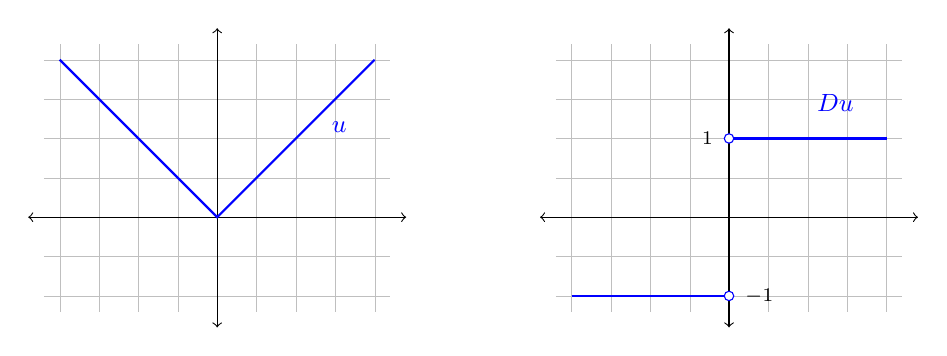
\begin{tikzpicture}[scale=1.0]
	\begin{scope}
		\draw[ultra thin, color=lightgray, step=0.5] (-2.2,-1.2) grid (2.2,2.2);
		\draw[<->] (-2.4,0) -- (2.4,0);
		\draw[<->] (0,-1.4) -- (0,2.4);
		\draw[thick, color=blue] (-2,2) -- (0,0) -- (2,2);
		\node[color=blue] at (1.55,1.15) {\small $u$};
	\end{scope}
	\begin{scope}[xshift=6.5cm]
		\draw[ultra thin, color=lightgray, step=0.5] (-2.2,-1.2) grid (2.2,2.2);
		\draw[<->] (-2.4,0) -- (2.4,0);
		\draw[<->] (0,-1.4) -- (0,2.4);
		\draw[thick, color=blue] (-2,-1) -- (0,-1);
		\draw[thick, color=blue] (0,1) -- (2,1);
		\draw[color=blue, fill=white] (0,-1) circle (0.06);
		\draw[color=blue, fill=white] (0,1) circle (0.06);
		\node[color=blue] at (1.35,1.45) {\small $Du$};
		\node[left] at (-0.08,1) {\scriptsize $1$};
		\node[right] at (0.08,-1) {\scriptsize $-1$};
	\end{scope}
\end{tikzpicture}
\end{center}
\end{example}

\subsection{Sobolev spaces via the Fourier transform}

On $\Omega=\R^n$ with $p = 2$ we can say something much sharper, because the Fourier transform turns differentiation into multiplication. Indeed for $f \in L^2(\R^n)$ we have $D^\alpha f \in L^2(\R^n)$ if and only if $\xi^\alpha\hat f(\xi)\in L^2(\R^n)$, by Lemma \ref{lem:tempft} and Plancherel. Since $\sum_{|\alpha|\le k}|\xi^\alpha|^2$ is comparable to $(1+|\xi|^2)^k$, this suggests a definition which makes sense for non-integer orders.

\begin{definition}
	For $s\in\R$, we say $u \in \Sch'(\R^n)$ belongs to $H^s(\R^n)$ if $\hat u \in L^2_{\mathrm{loc}}(\R^n)$ and
	$$\norm{u}_{H^s}^2 = \frac{1}{(2\pi)^n}\int_{\R^n}(1+|\xi|^2)^s|\hat u(\xi)|^2\dd\xi<\infty.$$
	This makes $H^s(\R^n)$ a Hilbert space with $\ip{u}{v}_{H^s}=(2\pi)^{-n}\int\ol{\hat u}\hat v(1+|\xi|^2)^s\dd\xi$.
\end{definition}

For $s \in \Z_{\ge0}$ we have $H^s(\R^n)=W^{s,2}(\R^n)$ with equivalent norms, by the remarks above. But now $s$ may be any real number: fractional orders measure fractional differentiability, and negative orders describe distributions rougher than functions. For instance $\delta_0 \in H^s(\R^n)$ exactly when $s < -n/2$, since $\hat{\delta_0}=1$ and $\int(1+|\xi|^2)^s\dd\xi<\infty$ iff $2s<-n$.

The Fourier description makes the following density statement almost trivial, and we shall use it repeatedly to reduce statements about $H^s$ to computations with Schwartz functions.

\begin{lemma}\label{lem:schwartzdense}
	For every $s \in \R$, the space $\Sch(\R^n)$ is dense in $H^s(\R^n)$.
\end{lemma}

\begin{proof}
	Let $u \in H^s(\R^n)$, so that $w = (1+|\xi|^2)^{s/2}\hat u \in L^2(\R^n)$. By Corollary \ref{cor:ccinftydense} choose $\psi \in C_c^\infty(\R^n)$ with $\norm{w - \psi}_{L^2}<(2\pi)^{n/2}\varepsilon$, and set
	$$v = \FF^{-1}\!\left[ (1+|\xi|^2)^{-s/2}\psi\right].$$
	The function $\xi\mapsto(1+|\xi|^2)^{-s/2}$ is smooth on all of $\R^n$, so $(1+|\xi|^2)^{-s/2}\psi \in C_c^\infty(\R^n)\subseteq\Sch(\R^n)$, whence $v \in \Sch(\R^n)$ by Corollary \ref{cor:fsiso}. And
	$$\norm{u-v}_{H^s}^2=\frac{1}{(2\pi)^n}\int_{\R^n}(1+|\xi|^2)^s\left|\hat u - \hat v\right|^2\dd\xi = \frac{1}{(2\pi)^n}\norm{w-\psi}^2_{L^2}<\varepsilon^2. \qedhere$$
\end{proof}

\subsection{The Sobolev embedding theorem}

Here is the theorem that makes Sobolev spaces worth the trouble.

\begin{theorem}[Sobolev embedding]\label{thm:sobolevembed}
	Let $k\in\Z_{\ge0}$ and $s > k + n/2$. If $f \in H^s(\R^n)$ then there is $f^*\in C^k(\R^n)$ with $f = f^*$ almost everywhere, and
	$$\sup_{x\in\R^n,|\alpha|\le k}|D^\alpha f^*(x)|\le c_{n,k,s}\norm{f}_{H^s}.$$
	We write $H^s(\R^n)\subseteq C^k(\R^n)$.
\end{theorem}

\begin{proof}
	Suppose first $f\in\Sch(\R^n)$. By the inversion theorem and Lemma \ref{lem:tempft},
	$$D^\alpha f(x)=\frac{i^{|\alpha|}}{(2\pi)^n}\int_{\R^n}e^{i(x\cdot\xi)}\xi^\alpha\hat f(\xi)\dd\xi,$$
	so by Cauchy--Schwarz, inserting and removing a factor $(1+|\xi|^2)^{s/2}$,
	$$|D^\alpha f(x)|\le\frac{1}{(2\pi)^n}\left(\int_{\R^n}(1+|\xi|^2)^s|\hat f(\xi)|^2\dd\xi\right)^{1/2}\left(\int_{\R^n}\frac{|\xi^\alpha|^2}{(1+|\xi|^2)^s}\dd\xi\right)^{1/2}.$$
	Since $|\alpha|\le k$ we have $|\xi^\alpha|^2\le c_k(1+|\xi|^2)^k$, so the second integral is at most
	$$c_k\int_{\R^n}\frac{\dd\xi}{(1+|\xi|^2)^{s-k}}=c^2_{k,n,s}<\infty$$
	precisely because $2(s-k)>n$. Hence $\sup_{x,|\alpha|\le k}|D^\alpha f(x)|\le c_{n,k,s}\norm{f}_{H^s}$ for $f\in\Sch(\R^n)$.

	For general $f \in H^s(\R^n)$, approximate: by Lemma \ref{lem:schwartzdense} there are $f_m\in\Sch(\R^n)$ with $f_m\to f$ in $H^s$, hence in $L^2$, and so (after passing to a subsequence) almost everywhere. The sequence $(f_m)$ is Cauchy in $H^s$, hence by the estimate Cauchy in $C^k(\R^n)$ with the uniform norm on all derivatives up to order $k$; that space is complete, so $f_m\to f^*$ in $C^k$. Since also $f_m\to f$ a.e., $f = f^*$ a.e.
\end{proof}

The moral is that \emph{differentiability can be bought with integrability, at an exchange rate of $n/2$ derivatives}. It is a genuinely surprising statement: membership of $H^s$ is a statement about integrals, and yet for $s$ large enough it forces pointwise regularity. Note also that the threshold is sharp: in $\R^n$ with $n \ge 2$, the function $\log\log(1+1/|x|)$ near the origin is in $H^{n/2}$ but unbounded, so $s = k+n/2$ will not do.

The general $L^p$ statement, which we quote, is a chart of the same phenomenon at other exponents.

\begin{theorem}[General Sobolev embeddings]\label{thm:sobolevchart}
	Let $\Omega\subseteq\R^n$ be a bounded domain with $C^1$ boundary, $k\ge1$ and $1\le p<\infty$.
	\begin{enumerate}[label=(\roman*)]
		\item If $kp<n$ then $W^{k,p}(\Omega)\subseteq L^q(\Omega)$ for $\frac1q=\frac1p-\frac kn$, continuously.
		\item If $kp>n$ then $W^{k,p}(\Omega)\subseteq C^{m,\gamma}(\ol\Omega)$, where $m=k-\lfloor n/p\rfloor-1$ and $\gamma\in(0,1)$ is determined by $n,k,p$.
		\item If $kp=n$ then $W^{k,p}(\Omega)\subseteq L^q(\Omega)$ for every $q<\infty$, but not in general for $q=\infty$.
	\end{enumerate}
\end{theorem}

\begin{center}
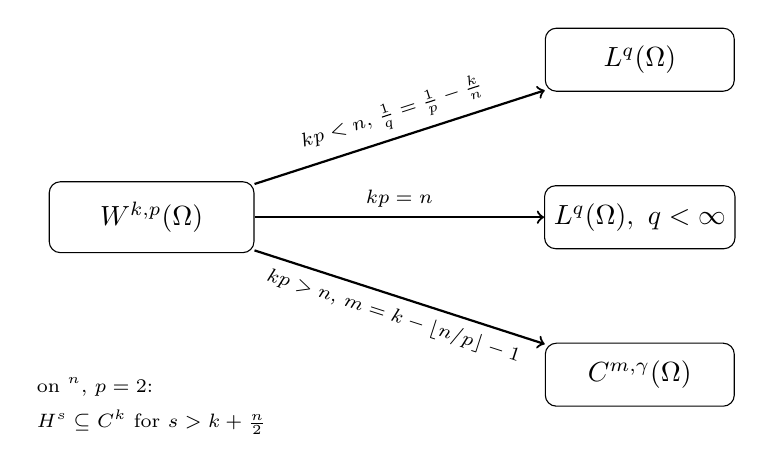
\begin{tikzpicture}[scale=1.0]
	\node[draw, rounded corners, minimum width=2.6cm, minimum height=0.9cm] (W) at (0,0) {$W^{k,p}(\Omega)$};
	\node[draw, rounded corners, minimum width=2.4cm, minimum height=0.8cm] (Lq) at (6.2,2.0) {$L^{q}(\Omega)$};
	\node[draw, rounded corners, minimum width=2.4cm, minimum height=0.8cm] (Lany) at (6.2,0) {$L^{q}(\Omega),\ q<\infty$};
	\node[draw, rounded corners, minimum width=2.4cm, minimum height=0.8cm] (C) at (6.2,-2.0) {$C^{m,\gamma}(\ol\Omega)$};
	\draw[->, thick] (W) -- node[above, sloped] {\scriptsize $kp<n$, $\frac1q=\frac1p-\frac kn$} (Lq);
	\draw[->, thick] (W) -- node[above] {\scriptsize $kp=n$} (Lany);
	\draw[->, thick] (W) -- node[below, sloped] {\scriptsize $kp>n$, $m=k-\lfloor n/p\rfloor-1$} (C);
	\node[align=left] at (0,-2.4) {\scriptsize on $\R^n$, $p=2$: \\[1pt] \scriptsize $H^s \subseteq C^k$ for $s>k+\frac n2$};
\end{tikzpicture}
\end{center}

\subsection{The spaces \texorpdfstring{$H_0^1(\Omega)$}{H10} and traces}

For boundary value problems we need to make sense of the restriction of a Sobolev function to $\partial\Omega$, which is a set of measure zero. Since elements of $H^s$ are only defined up to null sets, this requires an argument; the answer is that it can be done as soon as $s>1/2$.

\begin{theorem}[Trace theorem]\label{thm:trace}
	Let $s>1/2$. There is a bounded surjective linear map
	$$T : H^s(\R^n)\to H^{s-1/2}(\R^{n-1})$$
	with $Tf = f|_{\{x_n=0\}}$ for every $f \in \Sch(\R^n)$.
\end{theorem}

The proof (example sheet) is a computation with the Fourier transform: one shows that the partial transform of the restriction is obtained by integrating $\hat f$ in the $\xi_n$ variable, and estimates the result with Cauchy--Schwarz exactly as in Theorem \ref{thm:sobolevembed}. Note the loss of half a derivative, and note that $s>1/2$ is needed: an $H^{1/2}$ function has no well-defined trace. By combining with local coordinate changes one obtains a trace map onto sufficiently regular hypersurfaces, in particular onto the boundary of a Lipschitz domain.

\begin{definition}
	Let $\Omega\subseteq\R^n$ be open. Extending by zero, we regard $C_c^\infty(\Omega)\subseteq H^1(\R^n)$, and define $H_0^1(\Omega)$ to be the closure of $C_c^\infty(\Omega)$ in $H^1(\R^n)$.
\end{definition}

For $f\in C_c^\infty(\Omega)$, Plancherel gives the convenient formula
$$\norm{f}_{H^1}^2=\frac{1}{(2\pi)^n}\int_{\R^n}(1+|\xi|^2)|\hat f(\xi)|^2\dd\xi=\int_\Omega\left(|Df(x)|^2+|f(x)|^2\right)\dd x,$$
so $H_0^1(\Omega)$ is a Hilbert space with inner product
$$\ip{u}{v}_{H^1}=\int_\Omega \left(Du\cdot \ol{Dv}+\ol uv\right)\dd x.$$

Elements of $H_0^1(\Omega)$ vanish outside $\Omega$ and have zero trace on $\partial\Omega$. Indeed, if $\varphi\in C_c^\infty((\Omega^c)^\circ)$ then $\Lambda_\varphi(u)=\int_{\R^n}\varphi u$ vanishes for $u \in C_c^\infty(\Omega)$ and is continuous on $H^1(\R^n)$, so it vanishes on $H_0^1(\Omega)$ -- that is, every $u \in H_0^1(\Omega)$ vanishes a.e.\ on $\Omega^c$. And if $\partial\Omega$ is regular enough for the trace map $T : H^1 \to H^{1/2}(\partial\Omega)$ to be defined and bounded, then $Tu = 0$ for $u \in C_c^\infty(\Omega)$ and hence for all $u \in H_0^1(\Omega)$. So, informally:
$$H_0^1(\Omega)=\left\{ u \in H^1 : u = 0 \text{ on } \partial\Omega \text{ and outside }\Omega\right\},$$
and this is the space in which we shall pose the Dirichlet problem.

\subsection{Poincar\'e's inequality}

On $H_0^1(\Omega)$ with $\Omega$ bounded, the full $H^1$ norm is controlled by the gradient alone. This is a genuinely useful fact: it says that a function which vanishes on the boundary cannot be large without having a large derivative somewhere.

\begin{theorem}[Poincar\'e]\label{thm:poincare}
	Let $\Omega\subseteq\R^n$ be contained in a slab $\{0<x_1<d\}$. Then
	$$\norm{u}_{L^2(\Omega)}\le d\norm{Du}_{L^2(\Omega)} \quad \text{for all } u \in H_0^1(\Omega).$$
\end{theorem}

\begin{proof}
	By density it is enough to treat $u \in C_c^\infty(\Omega)$, which we extend by zero to the slab. For such $u$, the fundamental theorem of calculus in the $x_1$ direction gives
	$$u(x)=\int_0^{x_1}\partial_1u(t,x_2,\dots,x_n)\dd t,$$
	so by Cauchy--Schwarz
	$$|u(x)|^2\le x_1\int_0^{d}|\partial_1u(t,x')|^2\dd t \le d\int_0^d|\partial_1u(t,x')|^2\dd t,$$
	where $x'=(x_2,\dots,x_n)$. Integrating in $x_1$ over $(0,d)$ and then in $x'$ over $\R^{n-1}$,
	$$\int_\Omega|u|^2\dd x \le d^2\int_\Omega|\partial_1u|^2\dd x\le d^2\int_\Omega|Du|^2\dd x. \qedhere$$
\end{proof}

\begin{corollary}\label{cor:equivnorm}
	For $\Omega$ bounded, $\norm{Du}_{L^2(\Omega)}$ is a norm on $H_0^1(\Omega)$ equivalent to $\norm{u}_{H^1}$.
\end{corollary}

\begin{proof}
	Clearly $\norm{Du}_{L^2}\le\norm{u}_{H^1}$, and conversely $\norm{u}^2_{H^1}=\norm{Du}^2_{L^2}+\norm{u}^2_{L^2}\le(1+d^2)\norm{Du}^2_{L^2}$.
\end{proof}

Poincar\'e's inequality fails on all of $H^1(\Omega)$ -- constants are a counterexample -- and it fails on $H_0^1(\R^n)=H^1(\R^n)$, where there is no bounded direction. Boundedness of the domain, or at least of one direction, is essential.

\subsection{Rellich--Kondrachov}

Finally we come to the compactness theorem. Let $\Omega$ be open and bounded and let $(u_m)$ be a bounded sequence in $H_0^1(\Omega)$, say $\norm{u_m}_{H^1}\le K$. Since $H_0^1(\Omega)$ is a Hilbert space, hence reflexive, Corollary \ref{cor:reflexiveweak} gives a subsequence with $u_m\weakto u$ in $H_0^1(\Omega)$, and $\norm{u}_{H^1}\le K$. Moreover for $w \in L^2(\Omega)$ we have $|\ip{w}{v}_{L^2}|\le\norm{w}_{L^2}\norm{v}_{H^1}$, so $v \mapsto \ip{w}{v}_{L^2}$ is a bounded functional on $H_0^1(\Omega)$ and therefore $u_m\weakto u$ in $L^2(\Omega)$ as well. The theorem is that this convergence is in fact \emph{strong}.

\begin{theorem}[Rellich--Kondrachov]\label{thm:rellich}
	Let $\Omega\subseteq\R^n$ be open and bounded. Suppose $(u_m)\subseteq H_0^1(\Omega)$ with $\norm{u_m}_{H^1}\le K$ and $u_m\weakto u$ in $L^2(\Omega)$ for some $u \in H_0^1(\Omega)$. Then $u_m\to u$ strongly in $L^2(\Omega)$.
\end{theorem}

\begin{proof}
	Regard everything as defined on $\R^n$ by extension by zero. By Plancherel,
	$$\norm{u_m-u}_{L^2}^2=\frac{1}{(2\pi)^n}\int_{|\xi|<R}|\hat u_m-\hat u|^2\dd\xi+\frac{1}{(2\pi)^n}\int_{|\xi|\ge R}|\hat u_m-\hat u|^2\dd\xi,$$
	and we treat the two ranges differently. This is the standard division into low and high frequencies, and it is worth remembering: the high frequencies are killed by the derivative bound, the low frequencies by the weak convergence.

	\emph{High frequencies.} For $|\xi|\ge R$ we have $1 \le (1+|\xi|^2)/R^2$, so
	\begin{align*}
		\int_{|\xi|\ge R}|\hat u_m-\hat u|^2\dd\xi &\le\frac{2}{R^2}\int_{\R^n}(1+|\xi|^2)\left(|\hat u_m|^2+|\hat u|^2\right)\dd\xi \\
		&\le\frac{C}{R^2}\left(\norm{u_m}^2_{H^1}+\norm{u}^2_{H^1}\right)\le\frac{CK^2}{R^2},
	\end{align*}
	which we may make as small as we please by choosing $R$ large -- \emph{uniformly in $m$}.

	\emph{Low frequencies.} Fix such an $R$. Since $|\Omega|<\infty$, the function $x\mapsto e^{-i(x\cdot\xi)}$ lies in $L^2(\Omega)$ for each $\xi$, and $\hat u_m(\xi)=\ip{e_\xi}{u_m}_{L^2(\Omega)}$. So weak convergence in $L^2(\Omega)$ gives $\hat u_m(\xi)\to\hat u(\xi)$ pointwise. Moreover, by the Riemann--Lebesgue bound and Cauchy--Schwarz on the bounded set $\Omega$,
	$$|\hat u_m(\xi)-\hat u(\xi)|^2\le2\left(\norm{u_m}^2_{L^1}+\norm{u}^2_{L^1}\right)\le2|\Omega|\left(\norm{u_m}^2_{L^2}+\norm{u}^2_{L^2}\right)\le C',$$
	a constant, which is integrable on the ball $\{|\xi|<R\}$. Dominated convergence therefore gives
	$$\int_{|\xi|<R}|\hat u_m(\xi)-\hat u(\xi)|^2\dd\xi\longrightarrow 0 \quad\text{as } m \to\infty.$$
	Combining, $\limsup_m\norm{u_m-u}^2_{L^2}\le CK^2/R^2$ for every $R$, so the limit is $0$.
\end{proof}

\begin{corollary}\label{cor:rellichseq}
	Let $\Omega$ be open and bounded and let $(u_m)\subseteq H_0^1(\Omega)$ with $\norm{u_m}_{H^1}\le K$. Then there is a subsequence and $u \in H_0^1(\Omega)$ with $u_m\weakto u$ in $H^1$ and $u_m \to u$ strongly in $L^2$.
\end{corollary}

\begin{corollary}\label{cor:compactop}
	Let $\Omega$ be open and bounded and let $A : L^2(\Omega)\to H_0^1(\Omega)$ be bounded and linear. Then $A$, viewed as a map $L^2(\Omega)\to L^2(\Omega)$, is compact.
\end{corollary}

\begin{proof}
	If $\norm{u_m}_{L^2}\le K$ then $\norm{Au_m}_{H^1}\le\norm{A}K$, so $(Au_m)$ has an $L^2$-convergent subsequence by Corollary \ref{cor:rellichseq}.
\end{proof}

The inclusion $H_0^1(\Omega)\hookrightarrow L^2(\Omega)$ is thus a compact operator: the unit ball of $H_0^1$ is precompact in $L^2$. This is the compactness that we shall use to solve elliptic problems and to diagonalise the Laplacian. Note where boundedness of $\Omega$ entered -- twice, in fact -- and note that the result is false on $\R^n$, where the translates $\phi(\cdot - m)$ of a fixed bump are bounded in $H^1$ with no $L^2$-convergent subsequence.

\section{Applications to Elliptic Equations}\label{sec:pde}

We can now do what the whole course has been building towards. In this section $\Omega\subseteq\R^n$ is open and bounded, and we study the boundary value problem
$$\begin{cases} -\nabla^2u+u=f & \text{in }\Omega,\\ u = 0 & \text{on }\partial\Omega.\end{cases}$$
Classically one would ask for $u \in C^2(\Omega)\cap C^0(\ol\Omega)$ satisfying this pointwise, and proving that such a $u$ exists is hard. The modern strategy is to relax the problem until existence is easy, and then to work to show that the object produced is better than it had to be.

\begin{center}
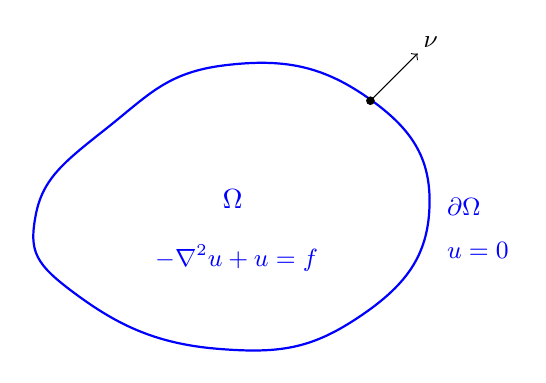
\begin{tikzpicture}[scale=1.0]
	\draw[thick, color=blue] plot[smooth cycle, tension=0.8] coordinates
		{(0,0) (1.8,-0.7) (3.6,-0.3) (4.5,1.1) (3.7,2.5) (1.9,2.9) (0.4,2.1) (-0.5,1.0)};
	\node[color=blue] at (2.0,1.2) {$\Omega$};
	\node[color=blue] at (2.05,1.2-0.75) {\small $-\nabla^2u+u=f$};
	\node[color=blue, right] at (4.6,1.1) {\small $\partial\Omega$};
	\node[color=blue, right] at (4.6,0.55) {\small $u=0$};
	% outward normal at a boundary point
	\fill (3.75,2.45) circle (0.055);
	\draw[->] (3.75,2.45) -- (4.35,3.05);
	\node[above right] at (4.3,3.0) {\small $\nu$};
\end{tikzpicture}
\end{center}

\subsection{Weak solutions}

Suppose for a moment that $u$ is a classical solution and $v \in C_c^\infty(\Omega)$. Multiplying by $\ol v$ and integrating by parts (no boundary term, as $v$ has compact support),
$$\int_\Omega\left( Du\cdot\ol{Dv}+u\ol v\right)\dd x = \int_\Omega f\ol v\dd x,$$
that is, $\ip{v}{u}_{H^1}=\ip{v}{f}_{L^2}$ in our notation. The left side makes sense for $u \in H^1$, and by continuity the identity extends from $v \in C_c^\infty(\Omega)$ to $v \in H_0^1(\Omega)$. This motivates the following.

\begin{definition}[Weak solution]
	Let $f \in L^2(\Omega)$. We say $u \in H_0^1(\Omega)$ is a \vocab{weak solution} of the boundary value problem if
	$$\ip{u}{v}_{H^1}=\ip{f}{v}_{L^2} \quad \text{for all } v \in H_0^1(\Omega).$$
\end{definition}

Note that the boundary condition is encoded in the requirement $u \in H_0^1(\Omega)$, not in a separate equation. Conversely, if $u$ is a weak solution then testing against $v \in C_c^\infty(\Omega)$ and integrating by parts shows that $-\nabla^2u+u=f$ holds in $\DD'(\Omega)$. So the notions match up as they should.

\begin{lemma}\label{lem:dirichletexist}
	For every $f \in L^2(\Omega)$ there is a unique weak solution $u \in H_0^1(\Omega)$, and $\norm{u}_{H^1}\le\norm{f}_{L^2}$.
\end{lemma}

\begin{proof}
	The map $\Lambda : v \mapsto \ip{f}{v}_{L^2}$ is linear, and bounded on $H_0^1(\Omega)$ since
	$$|\ip{f}{v}_{L^2}|\le\norm{f}_{L^2}\norm{v}_{L^2}\le\norm{f}_{L^2}\norm{v}_{H^1}.$$
	As $H_0^1(\Omega)$ is a Hilbert space, Theorem \ref{thm:rieszhilbert} provides a unique $u \in H_0^1(\Omega)$ with $\ip{u}{v}_{H^1}=\Lambda(v)$ for all $v$, and $\norm{u}_{H^1}=\norm{\Lambda}\le\norm{f}_{L^2}$.
\end{proof}

That is the entire existence proof. It is worth pausing to see how much was smuggled in: the completeness of $H_0^1$ (Riesz--Fischer), the identification of the $H^1$ inner product with the Dirichlet form (Plancherel), and the interpretation of the boundary condition (density of $C_c^\infty$). Each was a theorem, and together they reduce a partial differential equation to the observation that a Hilbert space is its own dual.

\begin{definition}
	Write $A : L^2(\Omega)\to H_0^1(\Omega)$ for the map $f \mapsto u$ given by Lemma \ref{lem:dirichletexist}, the \vocab{solution operator}.
\end{definition}

\begin{proposition}\label{prop:solop}
	$A$ is linear and bounded with $\norm{Af}_{H^1}\le\norm{f}_{L^2}$, and, regarded as a map $L^2(\Omega)\to L^2(\Omega)$, it is compact and Hermitian.
\end{proposition}

\begin{proof}
	Linearity: if $u = Af$, $w=Ag$ then for all $v$,
	$$\ip{u+aw}{v}_{H^1}=\ip{f}{v}_{L^2}+\ol a\ip{g}{v}_{L^2}=\ip{f+ag}{v}_{L^2},$$
	so $A(f+ag)=Af+aAg$ by uniqueness. Boundedness is Lemma \ref{lem:dirichletexist}; compactness follows from Corollary \ref{cor:compactop}. For the Hermitian property, with $u = Af$, $w = Ag$,
	$$\ip{f}{Ag}_{L^2}=\ip{f}{w}_{L^2}=\ol{\ip{w}{f}_{L^2}}=\ol{\ip{w}{u}_{H^1}}=\ip{u}{w}_{H^1}=\ip{Af}{g}_{L^2}. \qedhere$$
\end{proof}

\subsection{The Lax--Milgram theorem}

Lemma \ref{lem:dirichletexist} used the fact that the Dirichlet form is exactly the $H^1$ inner product. For a general elliptic operator this fails: the associated bilinear form is neither symmetric nor equal to an inner product. The following generalisation of the Riesz representation theorem is the standard remedy.

\begin{theorem}[Lax--Milgram]\label{thm:laxmilgram}
	Let $\Hil$ be a Hilbert space and $B : \Hil\times\Hil\to\C$ a sesquilinear form which is
	\begin{enumerate}[label=(\roman*)]
		\item \vocab{bounded}: $|B(u,v)|\le C\norm{u}\norm{v}$ for some $C>0$, and
		\item \vocab{coercive}: $|B(u,u)|\ge c\norm{u}^2$ for some $c>0$.
	\end{enumerate}
	Then for every $\Lambda \in \Hil'$ there is a unique $u \in \Hil$ with $B(u,v)=\Lambda(v)$ for all $v\in\Hil$, and $\norm{u}\le c^{-1}\norm{\Lambda}$.
\end{theorem}

\begin{proof}
	For fixed $u$, the map $v \mapsto \ol{B(u,v)}$ is a bounded linear functional, so by Theorem \ref{thm:rieszhilbert} there is a unique $Su \in \Hil$ with $B(u,v)=\ip{v}{Su}^-$; more conveniently, define $S : \Hil \to \Hil$ by $\ip{Su}{v}=B(u,v)$. Then $S$ is linear and bounded with $\norm{S}\le C$, by (i).

	Coercivity gives $c\norm{u}^2\le|B(u,u)|=|\ip{Su}{u}|\le\norm{Su}\norm{u}$, so $\norm{Su}\ge c\norm{u}$. Hence $S$ is injective with closed range: if $Su_m \to w$ then $(u_m)$ is Cauchy, so $u_m \to u$ and $Su = w$. If the range were not everything, there would be $0 \ne z \perp \operatorname{ran}S$, and then $c\norm{z}^2\le|B(z,z)|=|\ip{Sz}{z}|=0$, a contradiction. So $S$ is a bijection.

	Given $\Lambda$, Theorem \ref{thm:rieszhilbert} gives $w$ with $\Lambda(v)=\ip{w}{v}$, and $u = S^{-1}w$ satisfies $B(u,v)=\ip{Su}{v}=\ip{w}{v}=\Lambda(v)$. Uniqueness is injectivity of $S$, and the bound follows from $\norm{u}\le c^{-1}\norm{Su}=c^{-1}\norm{w}=c^{-1}\norm{\Lambda}$.
\end{proof}

\begin{example}
	Let $a_{ij},b,c$ be bounded measurable on $\Omega$ with $\sum_{ij}a_{ij}(x)\xi_i\xi_j\ge\theta|\xi|^2$ for some $\theta>0$ (\vocab{uniform ellipticity}), and consider
	$$Lu = -\sum_{i,j}D_i(a_{ij}D_ju)+cu.$$
	The associated form is $B(u,v)=\int_\Omega\left(\sum_{ij}a_{ij}D_ju\ol{D_iv}+cu\ol v\right)$, which is bounded on $H_0^1(\Omega)$, and coercive as soon as $c \ge 0$ (or, using Poincar\'e, whenever $c > -\theta/d^2$). So Theorem \ref{thm:laxmilgram} gives a unique weak solution of $Lu = f$ in $H_0^1(\Omega)$ for every $f \in L^2(\Omega)$. Note that $B$ need not be symmetric -- $a_{ij}\ne a_{ji}$ is allowed -- so the Riesz theorem alone would not have sufficed.
\end{example}

\subsection{Elliptic regularity}

Our weak solution has, so far, one weak derivative. The equation says more.

\begin{proposition}\label{prop:regularityRn}
	Let $s \in \R$ and $f \in H^s(\R^n)$. Then there is a unique $u \in H^{s+2}(\R^n)$ with $-\nabla^2u+u=f$ in $\Sch'(\R^n)$, and $\norm{u}_{H^{s+2}}=\norm{f}_{H^s}$.
\end{proposition}

\begin{proof}
	Taking Fourier transforms, the equation reads $(|\xi|^2+1)\hat u(\xi)=\hat f(\xi)$, so necessarily $\hat u = \hat f/(1+|\xi|^2)$, which defines a tempered distribution and hence a unique $u$. Then
	$$\norm{u}^2_{H^{s+2}}=\frac{1}{(2\pi)^n}\int(1+|\xi|^2)^{s+2}\frac{|\hat f(\xi)|^2}{(1+|\xi|^2)^2}\dd\xi=\norm{f}^2_{H^s}. \qedhere$$
\end{proof}

So on $\R^n$ the operator $-\nabla^2+1$ gains exactly two derivatives, which is the best possible and is the defining feature of a second-order elliptic operator. On a domain we obtain the same gain locally, by cutting off.

\begin{definition}
	For $s>0$ let $H^s_{\mathrm{loc}}(\Omega)=\{u\in L^2_{\mathrm{loc}}(\Omega) : \chi u \in H^s(\R^n)\text{ for all }\chi\in C_c^\infty(\Omega)\}$.
\end{definition}

Note that if $s>n/2+k$ and $u \in H^s_{\mathrm{loc}}(\Omega)$ then $u \in C^k(\Omega)$: given $U$ with $\ol U\subseteq\Omega$ compact, choose $\chi\in C_c^\infty(\Omega)$ with $\chi\equiv1$ on $U$; then $\chi u \in H^s(\R^n)\subseteq C^k(\R^n)$ by Theorem \ref{thm:sobolevembed}, and $\chi u = u$ on $U$.

\begin{theorem}[Interior elliptic regularity]\label{thm:ellipticreg}
	Let $u \in H_0^1(\Omega)$ be a weak solution of $-\nabla^2u+u=f$ with $f\in L^2(\Omega)$. Then $u \in H^2_{\mathrm{loc}}(\Omega)$. If moreover $f \in H^k_{\mathrm{loc}}(\Omega)\cap L^2(\Omega)$ then $u \in H^{k+2}_{\mathrm{loc}}(\Omega)$; and if $f \in C^\infty(\Omega)\cap L^2(\Omega)$ then $u \in C^\infty(\Omega)$ and the equation holds classically.
\end{theorem}

\begin{proof}
	Fix a compact $K\subseteq\Omega$ and $\chi_K\in C_c^\infty(\Omega)$ with $\chi_K\equiv1$ on $K$, and set $w = \chi_Ku$. For any $\varphi\in\Sch(\R^n)$ the function $v = \chi_K\varphi$ lies in $C_c^\infty(\Omega)\subseteq H_0^1(\Omega)$, so it is admissible as a test function. Substituting and moving the cut-off across the derivatives, which is legitimate by the Leibniz rule of Lemma \ref{lem:leibniz}, gives
	$$\int_{\R^n}\ol w(-\nabla^2\varphi+\varphi)\dd x = \int_{\R^n}\ol g\varphi\dd x, \qquad g = f\chi_K - 2Du\cdot D\chi_K-u\nabla^2\chi_K.$$
	So $w \in H^1(\R^n)$ solves $-\nabla^2w+w=g$ in $\Sch'(\R^n)$, and $g \in L^2 = H^0$ since $u \in H^1$ and $f \in L^2$. By Proposition \ref{prop:regularityRn}, $w \in H^2(\R^n)$. As $K$ was arbitrary, $u \in H^2_{\mathrm{loc}}(\Omega)$.

	Now bootstrap. If additionally $f \in H^1_{\mathrm{loc}}$, then the formula for $g$ shows $g\in H^1(\R^n)$ (each term now has one more derivative available), so $w \in H^3(\R^n)$ and $u\in H^3_{\mathrm{loc}}(\Omega)$. Iterating gives $u \in H^{k+2}_{\mathrm{loc}}(\Omega)$ whenever $f\in H^k_{\mathrm{loc}}(\Omega)\cap L^2(\Omega)$. If $f$ is smooth this holds for every $k$, so $u \in \bigcap_kC^k(\Omega)=C^\infty(\Omega)$ by the remark above, and a smooth distributional solution is a classical solution.
\end{proof}

This gain of regularity -- for free, from the equation alone -- is called \vocab{elliptic regularity}, and it is the reason the weak formulation is not a cheat. We solved a weakened problem and got a classical solution anyway.

\begin{remark}
	It is emphatically a property of elliptic operators, not of differential operators in general. The wave equation $u_{tt}-u_{xx}=0$ has the general solution $u(x,t)=u_+(x+t)+u_-(x-t)$, and if $u_\pm$ are merely continuous this is a perfectly good weak solution which is nowhere differentiable. Hyperbolic equations propagate singularities rather than smoothing them.
\end{remark}

\subsection{The Fredholm alternative and eigenvalues of the Laplacian}

Consider now the problem with a potential:
$$\begin{cases} -\nabla^2u+Vu = f & \text{in }\Omega, \\ u = 0 & \text{on }\partial\Omega,\end{cases}$$
with $V : \Omega \to \R$ smooth and bounded. The weak formulation is
$$\int_\Omega \left( Du\cdot\ol{Dv}+V u\ol v\right)\dd x = \int_\Omega f \ol v \dd x \quad \text{for all } v \in H_0^1(\Omega),$$
but now the left-hand side need not be an inner product, since $V$ may be negative. Instead of appealing to Lax--Milgram (which would need $V$ bounded below appropriately) we rewrite:
$$\int_\Omega\left(Du\cdot\ol{Dv}+u\ol v\right)\dd x = \int_\Omega\left((1-V)u+f\right)\ol v\dd x,$$
which says precisely $u = A\big(f+(1-V)u\big)$, or
$$(I - \mathcal{K})u = Af, \qquad \mathcal{K}u = A\big((1-V)u\big).$$
Since $u \mapsto (1-V)u$ is bounded on $L^2(\Omega)$ and $A : L^2 \to H_0^1$ is bounded, $\mathcal{K} : L^2(\Omega)\to L^2(\Omega)$ is compact by Corollary \ref{cor:compactop}. The Fredholm theory of compact operators now applies verbatim:

\begin{theorem}\label{thm:fredholm}
	Let $\Omega$ be open and bounded and $V$ smooth and bounded. Then exactly one of the following holds.
	\begin{enumerate}[label=(\roman*)]
		\item There is a non-zero $w \in H_0^1(\Omega)\cap C^\infty(\Omega)$ with $-\nabla^2w+Vw=0$.
		\item For every $f \in L^2(\Omega)$ there is a unique weak solution $u \in H_0^1(\Omega)$ of the boundary value problem.
	\end{enumerate}
\end{theorem}

\begin{proof}
	By the Fredholm alternative for the compact operator $\mathcal{K}$, either $(I-\mathcal{K})w=0$ for some $w \ne 0$, or $I - \mathcal{K}$ is a bijection of $L^2(\Omega)$. In the first case $w = A((1-V)w)$, so $w \in H_0^1(\Omega)$, and $w$ is a weak solution of the homogeneous problem; Theorem \ref{thm:ellipticreg} (applied with the potential term absorbed into the right-hand side, and bootstrapped) gives $w \in C^\infty(\Omega)$. In the second case, given $f$ set $u = (I-\mathcal{K})^{-1}Af$.
\end{proof}

The same circle of ideas produces the spectral decomposition of the Laplacian, which is one of the most-used theorems in mathematical physics.

\begin{theorem}\label{thm:eigenvalues}
	Let $\Omega\subseteq\R^n$ be open and bounded. There is an orthonormal basis $(w_k)_{k\ge1}$ of $L^2(\Omega)$ with $w_k \in H_0^1(\Omega)\cap C^\infty(\Omega)$ and
	$$-\nabla^2w_k=\lambda_kw_k \quad\text{in }\Omega,$$
	where $0\le\lambda_1\le\lambda_2\le\cdots$ and $\lambda_k\to\infty$.
\end{theorem}

\begin{proof}
	By Proposition \ref{prop:solop}, $A : L^2(\Omega)\to L^2(\Omega)$ is compact and Hermitian. By the spectral theorem for such operators, $\sigma(A)=\{0,\mu_1,\mu_2,\dots\}$ with $\mu_k$ real, accumulating only at $0$, and $L^2(\Omega)$ has an orthonormal basis of eigenvectors of $A$.

	Suppose $Aw = \mu w$ with $w \ne 0$. Then $w = \mu^{-1}Aw \in H_0^1(\Omega)$ provided $\mu \ne 0$, and indeed $\mu \ne 0$: for any $v \in H_0^1(\Omega)$ we have $\ip{w}{v}_{L^2}=\ip{Aw}{v}_{H^1}=\mu\ip{w}{v}_{H^1}$, and taking $v = w$ gives $\norm{w}_{L^2}^2=\mu\norm{w}^2_{H^1}$, which forces $\mu > 0$. So $w \in H_0^1(\Omega)$ is a weak solution of $-\nabla^2w+w=\mu^{-1}w$, and elliptic regularity (Theorem \ref{thm:ellipticreg}, bootstrapping through $H^1_{\mathrm{loc}}, H^3_{\mathrm{loc}}, H^5_{\mathrm{loc}},\dots$) gives $w \in C^\infty(\Omega)$. Rewriting with $\lambda = \mu^{-1}-1$ gives $-\nabla^2w=\lambda w$, and $\lambda \ge 0$ since $\mu\norm{w}_{H^1}^2 = \norm{w}_{L^2}^2 \le \norm{w}^2_{H^1}$. Finally $\mu_k \to 0$ translates into $\lambda_k\to\infty$.
\end{proof}

\begin{corollary}
	$\left(\sqrt2\sin(k\pi x)\right)_{k=1}^\infty$ is an orthonormal basis of $L^2((0,1))$.
\end{corollary}

\begin{proof}
	Take $\Omega = (0,1)$, where the eigenvalue problem $-w''=\lambda w$, $w(0)=w(1)=0$ has exactly the solutions $w_k=\sqrt2\sin(k\pi x)$ with $\lambda_k=k^2\pi^2$.
\end{proof}

That the classical Fourier sine series is an orthonormal basis is thus a corollary of Rellich--Kondrachov and the spectral theorem. This is a pleasingly indirect route to a classical fact, and unlike the classical proof it generalises: on any bounded domain whatever, however irregular, the Dirichlet eigenfunctions form a basis.

\subsection{The direct method in action}

Finally we return to the variational point of view of Section \ref{sec:direct}, and show that the solution of the Dirichlet problem is a minimiser of an energy.

\begin{proposition}\label{prop:dirichletmin}
	Let $f \in L^2(\Omega)$ and define $S : H_0^1(\Omega)\to\R$ by
	$$S[u]=\int_\Omega\left(|Du|^2+|u|^2-\ol fu-f\ol u\right)\dd x = \norm{u}^2_{H^1}-2\re\ip{f}{u}_{L^2}.$$
	Then $S$ attains its infimum, at a unique $w$, and $w$ is precisely the weak solution of the Dirichlet problem.
\end{proposition}

\begin{proof}
	\emph{Bounded below and coercive.} By Cauchy--Schwarz and $2ab \le a^2 + b^2$,
	$$S[u]\ge\norm{u}^2_{H^1}-2\norm{u}_{L^2}\norm{f}_{L^2}\ge\norm{u}^2_{H^1}-\tfrac12\norm{u}^2_{L^2}-2\norm{f}^2_{L^2}\ge\tfrac12\norm{u}^2_{H^1}-2\norm{f}^2_{L^2}.$$
	So $\sigma = \inf S > -\infty$, and any $u$ with $S[u]\le K$ has $\norm{u}^2_{H^1}\le2K+4\norm{f}^2_{L^2}$.

	\emph{Minimising sequence and weak limit.} Take $u_m$ with $S[u_m]\to\sigma$. By the above the sequence is bounded in $H_0^1(\Omega)$, so by Corollary \ref{cor:reflexiveweak} we may pass to a subsequence with $u_m\weakto w$ in $H_0^1(\Omega)$.

	\emph{Lower semicontinuity.} The norm is weakly lower semicontinuous, so $\norm{w}_{H^1}\le\liminf\norm{u_m}_{H^1}$; and $\ip{f}{\cdot}_{L^2}$ is a bounded functional on $H_0^1(\Omega)$, so $\re\ip{f}{u_m}\to\re\ip{f}{w}$. Hence
	$$S[w]=\norm{w}^2_{H^1}-2\re\ip{f}{w}\le\liminf_m\left(\norm{u_m}^2_{H^1}-2\re\ip{f}{u_m}\right)=\liminf_mS[u_m]=\sigma,$$
	and as $S[w]\ge\sigma$ we get $S[w]=\sigma$.

	\emph{Euler--Lagrange equation.} For $v \in H_0^1(\Omega)$ and $t \in \R$, expanding,
	$$S[w+tv]=S[w]+2t\left(\re\ip{w}{v}_{H^1}-\re\ip{f}{v}_{L^2}\right)+t^2\norm{v}^2_{H^1}.$$
	Since $t = 0$ is a minimum of this quadratic in $t$, the linear coefficient vanishes: $\re\ip{w}{v}_{H^1}=\re\ip{f}{v}_{L^2}$ for all $v$, and replacing $v$ by $iv$ gives the imaginary parts too. So $w$ is a weak solution, and conversely reading the expansion backwards shows any weak solution is a minimiser. Uniqueness now follows from Lemma \ref{lem:dirichletexist}, or directly from strict convexity of $S$.
\end{proof}

The last computation is the general phenomenon: \emph{critical points of an energy are weak solutions of its Euler--Lagrange equation}. What makes this valuable is that the direct method applies to functionals far more general than quadratic ones, where no Riesz representation theorem is available.

\begin{theorem}\label{thm:convexintegrand}
	Let $\Omega\subseteq\R^n$ be open and bounded, and let $L : \C^n\to\R$ be convex with
	$$L(z)\ge\gamma|z|^2-C \quad \text{for all }z,$$
	for some $\gamma, C>0$. Then $S[u]=\int_\Omega L(Du)\dd x$ attains its infimum on $H_0^1(\Omega)$.
\end{theorem}

\begin{proof}
	The growth condition gives $S[u]\ge\gamma\norm{Du}^2_{L^2}-C|\Omega|$, so sublevel sets of $S$ are bounded in $H_0^1(\Omega)$ by Poincar\'e's inequality (Corollary \ref{cor:equivnorm}), and $S$ is bounded below. Convexity of $L$ makes $u \mapsto S[u]$ convex, and it is strongly lower semicontinuous by Fatou's lemma applied along an $L^2$-convergent subsequence of gradients. Corollary \ref{cor:directconvex} applies.
\end{proof}

\begin{example}
	The functional
	$$u \mapsto \int_\Omega\left(1+|Du|^4\right)^{1/4}\dd x$$
	is not covered by any of our linear theory: its Euler--Lagrange equation is a quasilinear second-order PDE with no explicit solution and no useful integral representation. But the integrand is convex with the required growth (after adjusting for the quartic power on a bounded domain), so a minimiser exists. This is the direct method's raison d'\^etre: it produces solutions to problems that cannot be solved.
\end{example}

\begin{remark}
	Let us close by recalling the pattern of the argument, since it is the moral of the course. We wanted a solution to an equation. We could not find one directly, so we
	\begin{enumerate}[label=(\roman*)]
		\item reformulated the problem in a Banach space of functions, chosen so that the relevant estimate is an inequality between norms (Sobolev spaces);
		\item enlarged the notion of solution until existence became a compactness argument (weak solutions, weak topologies, Banach--Alaoglu);
		\item used convexity to ensure the limit object was still a solution (lower semicontinuity, the direct method);
		\item and then used the equation itself to prove that the object we had constructed was much better behaved than the construction guaranteed (elliptic regularity).
	\end{enumerate}
	Every step required a theorem, and every theorem required the machinery of measure, integration and functional analysis assembled in the earlier sections. That is what analysis of functions is for.
\end{remark}

